\chapter{Acceptance test of system}\label{app:acceptance_test}

The journal documents the acceptance test of the implemented system. The main goal of the trails is to replicate the system used in \autoref{app:journal_speaker_test} but implemented with the DSP as linkage between source and amplifier. The system is performed in a scaled environment where the the gain of the entire system is 3 dB lower than expected. This is done to protect the speaker against potential overloading.



\section{Setup}

The setup of this experiment are depicted in Figure \ref{figure:SpeakertestSetup}, where the equipment is cataloged in \autoref{tab:UsedEquipmentAcceptance}, and described as follows:

\begin{itemize}
\item Vibration and \gls{SPL} will be measured by a microphone at a distance 1 meter in accordance with IEC 60268-5 Sound System Equipment - Part 5: Loudspeaker
\item Vibration will be measured by a Brüel \& Kjear Type 4344 accelerometer, placed at the backplate of the lowest woofer.
\item The speaker will be driven by a Crown Studio Reference I amplifier.
\item The ADC/DAC will convert measurements from accelerometer and microphone and relay to a computer via SPDIF.
\item Both Accelerometer and Microphone is calibrated into outputting -35 dB at respectively 1 G and 94 dB \gls{SPL}.
\item All recordings are synchronised and timestamped by looping the test signal back into the converter.
\item The computer will be logging data with a RME HammerFall DIGI 96-PDST sound card and Adobe Audition.
\item The signal generator is a Brüel \& Kjear Type 1049 which will sweep from 2.4 kHz to 20 Hz with a speed of 80 Hz/s. Corresponding with the same signal in \autoref{app:journal_speaker_test}.
\begin{itemize}
	\item The signal will be logged in the ADC/DAC
	\item The Output from the DSP will be logged in the ADC/DAC
\end{itemize}
\item The adjustable gain for compensating the low voltage of the DSP is a Rostec LMA-4 Preamplifier.
\begin{itemize}
	\item The gain is adjusted to output 94 dB @1kHz with an input into the DSP of 0.5Volt RMS
	\item The Power amp is during calibration fixed to 6 dB.
\end{itemize}
\item The gain will be adjusted on the DSP
\end{itemize}

The reason of gain calibration is to mimic the trails made in \autoref{app:journal_speaker_test}. With the gain calibrated to same level, the DSP gain can be neglected.  Furthermore the speaker will be placed in the anechoic room to eliminate any external disturbances corresponding to the requirements demanded in the IEC 60268-5 standard.

\subsection*{Test Setup}

\begin{figure}[H]
	\centering
	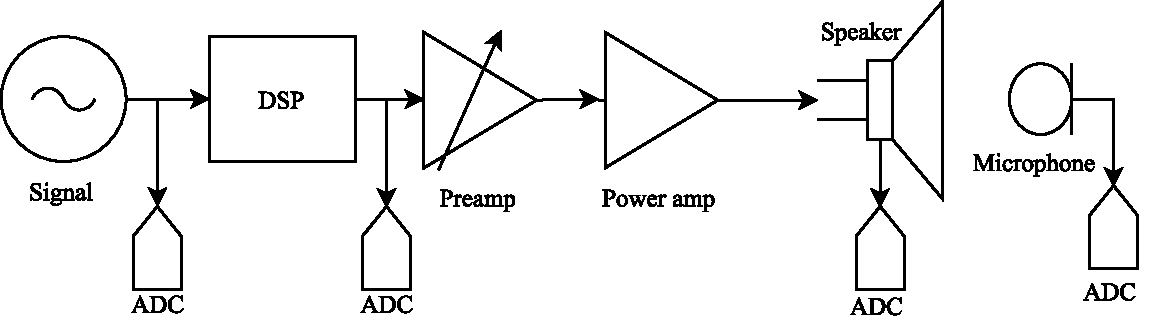
\includegraphics[width=1\textwidth]{figures/TestAcceptance}
	\caption{Schematic overview of the acceptance test setup}
	\label{fig:Acceptancetest}
\end{figure}


\subsection*{Equipment used and AAU-no.}

\begin{table}[H]
\centering
\ra{1.3}
\begin{tabular}{S[table-format=1]ccc} \toprule
    {Item} & {Description} & {AAU-no} \\ \bottomrule 
    1      &  Gras Type 40AZ microphone  & 75530   \\ 
    2      &  B \& K Accelerometer Type 4333  & 06596   \\ 
    3      &  Rostec LMA-4 Preamplifier  & 33094   \\
    4      &  Gras Type 26CC Preamplifier  & 75581   \\
    5      &  B \& K JJ2617 Accelerometer preamplifier & NaN   \\
    6      &  B \& K Power Supply 2805  & 64667  \\
    7      &  Crown Studio Reference I Amplifier & 52614   \\
    8      &  BEHRINGER digital A/D \& D/A Converter - Model ADA8000   & 56545   \\
    9      &  B \& K Accelerometer calibrator 4291 & 64668   \\
    10     &  B \& K Microphone calibrator 4231 & 78301   \\
    11     &  RME HammerFall DIGI 96-PDST sound card & 60919  \\
    12     &  Passive Dali Zensor 5 AX & NaN  \\ \bottomrule 
\end{tabular}
\caption{Table over equipment used in the test}
\label{tab:UsedEquipmentAcceptance}
\end{table}
\vspace{-5mm}


\section{Procedure}\label{sec:SpeakerTestProcedure1}

The producer for this experiment is described as follows:
\vspace{-5mm}
\begin{enumerate}
\item The poweramplifier is fixed at a gain of +19 dB
\item Vacate the anechoic room and seal the room.
\item Start recording in Adobe Audition for:
\begin{itemize}
\item Input signal and DSP output signal
\item Microphone and Accelerometer
\end{itemize}
\item Play the sweep into the dsp at following signal levels (in RMS)
\begin{enumerate}
	\item 223 mV (-7 dB)
	\item 250 mV (-6 dB)
	\item 281 mV (-5 dB)
	\item 315 mV (-4 dB)
	\item 353 mV (-3 dB)
	\item 397 mV (-2 dB)
	\item 445 mV (-1 dB)
	\item 500 mV ( 0 dB) 
\end{enumerate}
\item After sweep, stop recording all channels
\item Save recordings as \path{.wav} file
\item Repeat step 2 through 6 for the different gain levels in the dsp.
\end{enumerate}



%\begin{figure}[H]
%\centering
%\tikzsetnextfilename{linear_freq_sweep}
%% This file was created by matlab2tikz.
%
%The latest updates can be retrieved from
%  http://www.mathworks.com/matlabcentral/fileexchange/22022-matlab2tikz-matlab2tikz
%where you can also make suggestions and rate matlab2tikz.
%
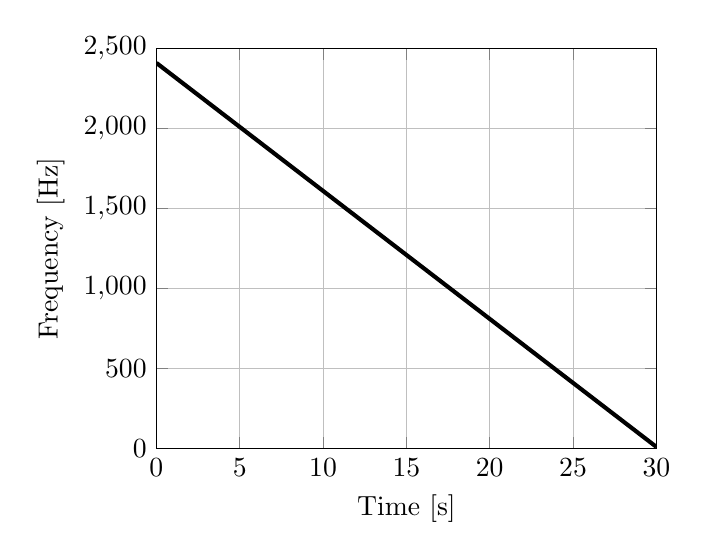
\begin{tikzpicture}

\begin{axis}[%
width=2.5in,
height=2in,
at={(1.011in,0.642in)},
scale only axis,
xmin=0,
xmax=30,
xmajorgrids,
ymin=0,
ymax=2500,
ymajorgrids,
xlabel={Time [s]},
ylabel={Frequency [Hz]},
axis background/.style={fill=white}
]
\addplot [color=black,solid,line width=1.5pt,forget plot]
  table[row sep=crcr]{%
0	2410\\
0.1	2402\\
0.2	2394\\
0.3	2386\\
0.4	2378\\
0.5	2370\\
0.6	2362\\
0.7	2354\\
0.8	2346\\
0.9	2338\\
1	2330\\
1.1	2322\\
1.2	2314\\
1.3	2306\\
1.4	2298\\
1.5	2290\\
1.6	2282\\
1.7	2274\\
1.8	2266\\
1.9	2258\\
2	2250\\
2.1	2242\\
2.2	2234\\
2.3	2226\\
2.4	2218\\
2.5	2210\\
2.6	2202\\
2.7	2194\\
2.8	2186\\
2.9	2178\\
3	2170\\
3.1	2162\\
3.2	2154\\
3.3	2146\\
3.4	2138\\
3.5	2130\\
3.6	2122\\
3.7	2114\\
3.8	2106\\
3.9	2098\\
4	2090\\
4.1	2082\\
4.2	2074\\
4.3	2066\\
4.4	2058\\
4.5	2050\\
4.6	2042\\
4.7	2034\\
4.8	2026\\
4.9	2018\\
5	2010\\
5.1	2002\\
5.2	1994\\
5.3	1986\\
5.4	1978\\
5.5	1970\\
5.6	1962\\
5.7	1954\\
5.8	1946\\
5.9	1938\\
6	1930\\
6.1	1922\\
6.2	1914\\
6.3	1906\\
6.4	1898\\
6.5	1890\\
6.6	1882\\
6.7	1874\\
6.8	1866\\
6.9	1858\\
7	1850\\
7.1	1842\\
7.2	1834\\
7.3	1826\\
7.4	1818\\
7.5	1810\\
7.6	1802\\
7.7	1794\\
7.8	1786\\
7.9	1778\\
8	1770\\
8.1	1762\\
8.2	1754\\
8.3	1746\\
8.4	1738\\
8.5	1730\\
8.6	1722\\
8.7	1714\\
8.8	1706\\
8.9	1698\\
9	1690\\
9.1	1682\\
9.2	1674\\
9.3	1666\\
9.4	1658\\
9.5	1650\\
9.6	1642\\
9.7	1634\\
9.8	1626\\
9.9	1618\\
10	1610\\
10.1	1602\\
10.2	1594\\
10.3	1586\\
10.4	1578\\
10.5	1570\\
10.6	1562\\
10.7	1554\\
10.8	1546\\
10.9	1538\\
11	1530\\
11.1	1522\\
11.2	1514\\
11.3	1506\\
11.4	1498\\
11.5	1490\\
11.6	1482\\
11.7	1474\\
11.8	1466\\
11.9	1458\\
12	1450\\
12.1	1442\\
12.2	1434\\
12.3	1426\\
12.4	1418\\
12.5	1410\\
12.6	1402\\
12.7	1394\\
12.8	1386\\
12.9	1378\\
13	1370\\
13.1	1362\\
13.2	1354\\
13.3	1346\\
13.4	1338\\
13.5	1330\\
13.6	1322\\
13.7	1314\\
13.8	1306\\
13.9	1298\\
14	1290\\
14.1	1282\\
14.2	1274\\
14.3	1266\\
14.4	1258\\
14.5	1250\\
14.6	1242\\
14.7	1234\\
14.8	1226\\
14.9	1218\\
15	1210\\
15.1	1202\\
15.2	1194\\
15.3	1186\\
15.4	1178\\
15.5	1170\\
15.6	1162\\
15.7	1154\\
15.8	1146\\
15.9	1138\\
16	1130\\
16.1	1122\\
16.2	1114\\
16.3	1106\\
16.4	1098\\
16.5	1090\\
16.6	1082\\
16.7	1074\\
16.8	1066\\
16.9	1058\\
17	1050\\
17.1	1042\\
17.2	1034\\
17.3	1026\\
17.4	1018\\
17.5	1010\\
17.6	1002\\
17.7	994\\
17.8	986\\
17.9	978\\
18	970\\
18.1	962\\
18.2	954\\
18.3	946\\
18.4	938\\
18.5	930\\
18.6	922\\
18.7	914\\
18.8	906\\
18.9	898\\
19	890\\
19.1	882\\
19.2	874\\
19.3	866\\
19.4	858\\
19.5	850\\
19.6	842\\
19.7	834\\
19.8	826\\
19.9	818\\
20	810\\
20.1	802\\
20.2	794\\
20.3	786\\
20.4	778\\
20.5	770\\
20.6	762\\
20.7	754\\
20.8	746\\
20.9	738\\
21	730\\
21.1	722\\
21.2	714\\
21.3	706\\
21.4	698\\
21.5	690\\
21.6	682\\
21.7	674\\
21.8	666\\
21.9	658\\
22	650\\
22.1	642\\
22.2	634\\
22.3	626\\
22.4	618\\
22.5	610\\
22.6	602\\
22.7	594\\
22.8	586\\
22.9	578\\
23	570\\
23.1	562\\
23.2	554\\
23.3	546\\
23.4	538\\
23.5	530\\
23.6	522\\
23.7	514\\
23.8	506\\
23.9	498\\
24	490\\
24.1	482\\
24.2	474\\
24.3	466\\
24.4	458\\
24.5	450\\
24.6	442\\
24.7	434\\
24.8	426\\
24.9	418\\
25	410\\
25.1	402\\
25.2	394\\
25.3	386\\
25.4	378\\
25.5	370\\
25.6	362\\
25.7	354\\
25.8	346\\
25.9	338\\
26	330\\
26.1	322\\
26.2	314\\
26.3	306\\
26.4	298\\
26.5	290\\
26.6	282\\
26.7	274\\
26.8	266\\
26.9	258\\
27	250\\
27.1	242\\
27.2	234\\
27.3	226\\
27.4	218\\
27.5	210\\
27.6	202\\
27.7	194\\
27.8	186\\
27.9	178\\
28	170\\
28.1	162\\
28.2	154\\
28.3	146\\
28.4	138\\
28.5	130\\
28.6	122\\
28.7	114\\
28.8	106\\
28.9	98\\
29	90\\
29.1	82\\
29.2	74\\
29.3	66\\
29.4	58\\
29.5	50\\
29.6	42\\
29.7	34\\
29.8	26\\
29.9	18\\
30	10\\
};
\end{axis}
\end{tikzpicture}%
%\caption{}
%\label{fig:linear_freq_sweep}
%\end{figure}


\section{Data Extraction}

8 Different measurements were taken with different amplification levels.

The recordings can be found on:\\
\scalebox{0.7}{
\path{CD://Maalinger/Maalinger230516 - Acceptance Test/}}
And is indexed in folders \scalebox{0.8}{\path{Measure_X}}, where X corresponds to the test number. Every measurements inside is denoted as:
\begin{itemize}
\item Accelerometer on driver: \scalebox{0.8}{\path{Accelerometer_0XX}}
\item Input Signal: \scalebox{0.8}{\path{Input_0XX}}
\item Microphone: \scalebox{0.8}{\path{Microphone_0XX}}
\item DPS Output signal: \scalebox{0.8}{\path{DSP_Output_0XX}}
\end{itemize}
\vspace*{-5mm}
The Script used to create all graphs are located at:\\
\scalebox{0.7}{
\path{CD://Maalinger/Maalinger030316 - Loudspeaker test/Measurements030316/downsampling_graph.m} and \path{FFT.m}}\\

\subsection{Raw Data}
The raw data is plotted showing the amplitude according to the time. It shows the characteristic of the same signal recorded in \autoref{app:journal_speaker_test}. Only three trials are showed to give an illustration of the increase in amplitude.
\begin{figure}[H]
	\centering
	\tikzsetnextfilename{Driver2}
	% This file was created by matlab2tikz.
%
%The latest updates can be retrieved from
%  http://www.mathworks.com/matlabcentral/fileexchange/22022-matlab2tikz-matlab2tikz
%where you can also make suggestions and rate matlab2tikz.
%
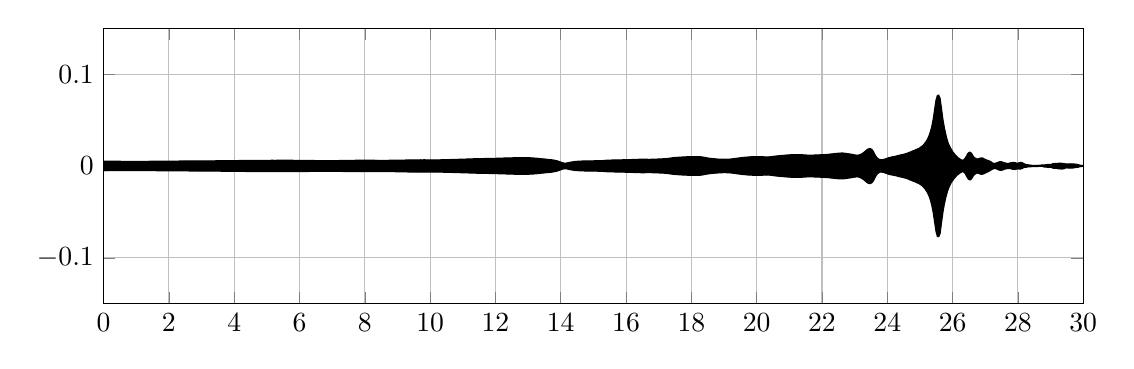
\begin{tikzpicture}

\begin{axis}[%
width=5.521in,
height=2in,
at={(0.758in,0.481in)},
xmin=0,
xmax=30,
xmajorgrids,
ymin=-0.15,
ymax=0.15,
ymajorgrids,
axis background/.style={fill=white}
]
\addplot[fill=black,draw=black,forget plot] plot table[row sep=crcr]{%
2.08333333333333e-05	0.00511908531188965\\
0.0425739952718676	0.005157470703125\\
0.0851271572104019	0.0051274299621582\\
0.127680319148936	0.00513732433319092\\
0.17023348108747	0.00513982772827148\\
0.212786643026005	0.00513327121734619\\
0.255339804964539	0.00510704517364502\\
0.297892966903073	0.00513815879821777\\
0.340446128841608	0.00511229038238525\\
0.382999290780142	0.00511360168457031\\
0.425552452718676	0.00509035587310791\\
0.46810561465721	0.00509989261627197\\
0.510658776595745	0.0050818920135498\\
0.553211938534279	0.00506234169006348\\
0.595765100472813	0.00506699085235596\\
0.638318262411347	0.0050661563873291\\
0.680871424349882	0.00504434108734131\\
0.723424586288416	0.00501227378845215\\
0.76597774822695	0.00503182411193848\\
0.808530910165485	0.00503897666931152\\
0.851084072104019	0.0050346851348877\\
0.893637234042553	0.00502979755401611\\
0.936190395981088	0.00503051280975342\\
0.978743557919622	0.0050588846206665\\
1.02129671985816	0.00504136085510254\\
1.06384988179669	0.00505304336547852\\
1.10640304373522	0.00503635406494141\\
1.14895620567376	0.0050663948059082\\
1.19150936761229	0.00503981113433838\\
1.23406252955083	0.00503933429718018\\
1.27661569148936	0.00506138801574707\\
1.3191688534279	0.00505185127258301\\
1.36172201536643	0.00504517555236816\\
1.40427517730496	0.00508773326873779\\
1.4468283392435	0.00506186485290527\\
1.48938150118203	0.00512361526489258\\
1.53193466312057	0.00510311126708984\\
1.5744878250591	0.00513827800750732\\
1.61704098699764	0.00513064861297607\\
1.65959414893617	0.00514745712280273\\
1.7021473108747	0.00517833232879639\\
1.74470047281324	0.00520122051239014\\
1.78725363475177	0.0051957368850708\\
1.82980679669031	0.00520873069763184\\
1.87235995862884	0.00522172451019287\\
1.91491312056738	0.00523662567138672\\
1.95746628250591	0.005240797996521\\
2.00001944444444	0.00526094436645508\\
2.04257260638298	0.00531005859375\\
2.08512576832151	0.00530004501342773\\
2.12767893026005	0.00531268119812012\\
2.17023209219858	0.0053025484085083\\
2.21278525413712	0.00531387329101563\\
2.25533841607565	0.00530898571014404\\
2.29789157801418	0.00534069538116455\\
2.34044473995272	0.00537323951721191\\
2.38299790189125	0.00535845756530762\\
2.42555106382979	0.0053861141204834\\
2.46810422576832	0.0053715705871582\\
2.51065738770686	0.00542116165161133\\
2.55321054964539	0.00540816783905029\\
2.59576371158392	0.00542199611663818\\
2.63831687352246	0.0054391622543335\\
2.68087003546099	0.00545692443847656\\
2.72342319739953	0.00546085834503174\\
2.76597635933806	0.00545108318328857\\
2.8085295212766	0.00548338890075684\\
2.85108268321513	0.00548028945922852\\
2.89363584515366	0.00546526908874512\\
2.9361890070922	0.00547075271606445\\
2.97874216903073	0.00549590587615967\\
3.02129533096927	0.00553667545318604\\
3.0638484929078	0.00551843643188477\\
3.10640165484634	0.00555849075317383\\
3.14895481678487	0.00557589530944824\\
3.1915079787234	0.00556671619415283\\
3.23406114066194	0.00557291507720947\\
3.27661430260047	0.00556766986846924\\
3.31916746453901	0.00557804107666016\\
3.36172062647754	0.00561273097991943\\
3.40427378841608	0.00560176372528076\\
3.44682695035461	0.0056302547454834\\
3.48938011229314	0.0056377649307251\\
3.53193327423168	0.00565564632415771\\
3.57448643617021	0.00568532943725586\\
3.61703959810875	0.00568020343780518\\
3.65959276004728	0.00572192668914795\\
3.70214592198582	0.00570118427276611\\
3.74469908392435	0.00574707984924316\\
3.78725224586288	0.00576865673065186\\
3.82980540780142	0.005767822265625\\
3.87235856973995	0.00579583644866943\\
3.91491173167849	0.00579166412353516\\
3.95746489361702	0.00580799579620361\\
4.00001805555556	0.00581538677215576\\
4.04257121749409	0.00584256649017334\\
4.08512437943262	0.00588428974151611\\
4.12767754137116	0.00588560104370117\\
4.17023070330969	0.00589430332183838\\
4.21278386524823	0.00590348243713379\\
4.25533702718676	0.00594067573547363\\
4.29789018912529	0.00592553615570068\\
4.34044335106383	0.00594091415405273\\
4.38299651300236	0.00596678256988525\\
4.4255496749409	0.00598776340484619\\
4.46810283687943	0.00601744651794434\\
4.51065599881797	0.00602161884307861\\
4.5532091607565	0.0060276985168457\\
4.59576232269503	0.00602662563323975\\
4.63831548463357	0.00604486465454102\\
4.6808686465721	0.00607025623321533\\
4.72342180851064	0.00605690479278564\\
4.76597497044917	0.00610077381134033\\
4.80852813238771	0.00612258911132813\\
4.85108129432624	0.0061107873916626\\
4.89363445626477	0.00611662864685059\\
4.93618761820331	0.00613296031951904\\
4.97874078014184	0.00611782073974609\\
5.02129394208038	0.00612950325012207\\
5.06384710401891	0.00612866878509521\\
5.10640026595745	0.0061575174331665\\
5.14895342789598	0.00616872310638428\\
5.19150658983452	0.00616919994354248\\
5.23405975177305	0.00615298748016357\\
5.27661291371158	0.00615584850311279\\
5.31916607565012	0.00617766380310059\\
5.36171923758865	0.00618886947631836\\
5.40427239952719	0.00619041919708252\\
5.44682556146572	0.00618433952331543\\
5.48937872340426	0.00618124008178711\\
5.53193188534279	0.00616204738616943\\
5.57448504728132	0.00617420673370361\\
5.61703820921986	0.00617754459381104\\
5.65959137115839	0.00618135929107666\\
5.70214453309693	0.00617098808288574\\
5.74469769503546	0.00617218017578125\\
5.787250856974	0.00617301464080811\\
5.82980401891253	0.00614452362060547\\
5.87235718085106	0.00611531734466553\\
5.9149103427896	0.00611543655395508\\
5.95746350472813	0.00610160827636719\\
6.00001666666667	0.00610089302062988\\
6.0425698286052	0.00610840320587158\\
6.08512299054374	0.00605452060699463\\
6.12767615248227	0.00605738162994385\\
6.1702293144208	0.00600779056549072\\
6.21278247635934	0.00600481033325195\\
6.25533563829787	0.00597274303436279\\
6.29788880023641	0.00595104694366455\\
6.34044196217494	0.00593674182891846\\
6.38299512411347	0.00592005252838135\\
6.42554828605201	0.00588977336883545\\
6.46810144799054	0.0058896541595459\\
6.51065460992908	0.00586163997650146\\
6.55320777186761	0.00582993030548096\\
6.59576093380615	0.00582337379455566\\
6.63831409574468	0.0057908296585083\\
6.68086725768321	0.00576961040496826\\
6.72342041962175	0.00574290752410889\\
6.76597358156028	0.00574243068695068\\
6.80852674349882	0.00571238994598389\\
6.85107990543735	0.0057302713394165\\
6.89363306737589	0.00570189952850342\\
6.93618622931442	0.00569808483123779\\
6.97873939125296	0.0057370662689209\\
7.02129255319149	0.00576698780059814\\
7.06384571513002	0.00576496124267578\\
7.10639887706856	0.00578999519348145\\
7.14895203900709	0.00584137439727783\\
7.19150520094563	0.00587165355682373\\
7.23405836288416	0.00590801239013672\\
7.27661152482269	0.00598061084747314\\
7.31916468676123	0.00596940517425537\\
7.36171784869976	0.00599408149719238\\
7.4042710106383	0.00601661205291748\\
7.44682417257683	0.00603854656219482\\
7.48937733451537	0.00607752799987793\\
7.5319304964539	0.00611376762390137\\
7.57448365839243	0.00612759590148926\\
7.61703682033097	0.00612497329711914\\
7.6595899822695	0.0061420202255249\\
7.70214314420804	0.00616204738616943\\
7.74469630614657	0.00619089603424072\\
7.78724946808511	0.00617849826812744\\
7.82980263002364	0.00616919994354248\\
7.87235579196217	0.00618600845336914\\
7.91490895390071	0.00617623329162598\\
7.95746211583924	0.00619924068450928\\
8.00001527777778	0.00620222091674805\\
8.04256843971631	0.00624048709869385\\
8.08512160165485	0.00620675086975098\\
8.12767476359338	0.00621354579925537\\
8.17022792553192	0.00621044635772705\\
8.21278108747045	0.00621426105499268\\
8.25533424940898	0.00620138645172119\\
8.29788741134752	0.00617086887359619\\
8.34044057328605	0.0061492919921875\\
8.38299373522459	0.00616514682769775\\
8.42554689716312	0.00612783432006836\\
8.46810005910165	0.00615501403808594\\
8.51065322104019	0.00611293315887451\\
8.55320638297872	0.0061107873916626\\
8.59575954491726	0.00612878799438477\\
8.63831270685579	0.00613880157470703\\
8.68086586879433	0.00613999366760254\\
8.72341903073286	0.00615501403808594\\
8.76597219267139	0.00618171691894531\\
8.80852535460993	0.00618219375610352\\
8.85107851654846	0.00621592998504639\\
8.893631678487	0.00625145435333252\\
8.93618484042553	0.00626301765441895\\
8.97873800236407	0.00628018379211426\\
9.0212911643026	0.00627684593200684\\
9.06384432624114	0.00633704662322998\\
9.10639748817967	0.00634157657623291\\
9.1489506501182	0.00635945796966553\\
9.19150381205674	0.00639116764068604\\
9.23405697399527	0.00643455982208252\\
9.27661013593381	0.00645220279693604\\
9.31916329787234	0.00649082660675049\\
9.36171645981088	0.00650417804718018\\
9.40426962174941	0.00653517246246338\\
9.44682278368794	0.00656521320343018\\
9.48937594562648	0.00660693645477295\\
9.53192910756501	0.00662446022033691\\
9.57448226950355	0.00664603710174561\\
9.61703543144208	0.00664782524108887\\
9.65958859338062	0.00668454170227051\\
9.70214175531915	0.00670921802520752\\
9.74469491725768	0.00668239593505859\\
9.78724807919622	0.00670409202575684\\
9.82980124113475	0.00672531127929688\\
9.87235440307329	0.0066683292388916\\
9.91490756501182	0.00665521621704102\\
9.95746072695036	0.0066523551940918\\
10.0000138888889	0.00663864612579346\\
10.0425670508274	0.00662267208099365\\
10.085120212766	0.00662577152252197\\
10.1276733747045	0.00663197040557861\\
10.170226536643	0.0066293478012085\\
10.2127796985816	0.00662577152252197\\
10.2553328605201	0.00665748119354248\\
10.2978860224586	0.00668108463287354\\
10.3404391843972	0.00672781467437744\\
10.3829923463357	0.00673449039459229\\
10.4255455082742	0.00677967071533203\\
10.4680986702128	0.00682806968688965\\
10.5106518321513	0.00689518451690674\\
10.5532049940898	0.00690901279449463\\
10.5957581560284	0.00695037841796875\\
10.6383113179669	0.00700652599334717\\
10.6808644799054	0.00703966617584229\\
10.723417641844	0.00709342956542969\\
10.7659708037825	0.00712478160858154\\
10.808523965721	0.00720775127410889\\
10.8510771276596	0.00722730159759521\\
10.8936302895981	0.00729072093963623\\
10.9361834515366	0.00732696056365967\\
10.9787366134752	0.00739002227783203\\
11.0212897754137	0.00741791725158691\\
11.0638429373522	0.00748777389526367\\
11.1063960992908	0.00752449035644531\\
11.1489492612293	0.00757277011871338\\
11.1915024231678	0.0076291561126709\\
11.2340555851064	0.00765800476074219\\
11.2766087470449	0.00768172740936279\\
11.3191619089835	0.00780510902404785\\
11.361715070922	0.00780856609344482\\
11.4042682328605	0.00783646106719971\\
11.4468213947991	0.00788748264312744\\
11.4893745567376	0.00789988040924072\\
11.5319277186761	0.00795161724090576\\
11.5744808806147	0.00801181793212891\\
11.6170340425532	0.0080183744430542\\
11.6595872044917	0.00807011127471924\\
11.7021403664303	0.0081021785736084\\
11.7446935283688	0.00813567638397217\\
11.7872466903073	0.00812971591949463\\
11.8297998522459	0.0081932544708252\\
11.8723530141844	0.00820529460906982\\
11.9149061761229	0.00823879241943359\\
11.9574593380615	0.00825619697570801\\
12.0000125	0.00832831859588623\\
12.0425656619385	0.00837266445159912\\
12.0851188238771	0.00838065147399902\\
12.1276719858156	0.00843846797943115\\
12.1702251477541	0.00850498676300049\\
12.2127783096927	0.00853443145751953\\
12.2553314716312	0.00863218307495117\\
12.2978846335697	0.00869262218475342\\
12.3404377955083	0.00872397422790527\\
12.3829909574468	0.00873851776123047\\
12.4255441193853	0.00881457328796387\\
12.4680972813239	0.00887799263000488\\
12.5106504432624	0.00886297225952148\\
12.5532036052009	0.00892508029937744\\
12.5957567671395	0.00894427299499512\\
12.638309929078	0.00899147987365723\\
12.6808630910165	0.00902092456817627\\
12.7234162529551	0.0090256929397583\\
12.7659694148936	0.00906562805175781\\
12.8085225768322	0.00909113883972168\\
12.8510757387707	0.00911200046539307\\
12.8936289007092	0.00910401344299316\\
12.9361820626478	0.00903439521789551\\
12.9787352245863	0.00905323028564453\\
13.0212883865248	0.00897479057312012\\
13.0638415484634	0.00890588760375977\\
13.1063947104019	0.0088423490524292\\
13.1489478723404	0.00874316692352295\\
13.191501034279	0.00858163833618164\\
13.2340541962175	0.00842511653900146\\
13.276607358156	0.00836801528930664\\
13.3191605200946	0.00819206237792969\\
13.3617136820331	0.00802290439605713\\
13.4042668439716	0.00788652896881104\\
13.4468200059102	0.00772547721862793\\
13.4893731678487	0.00759446620941162\\
13.5319263297872	0.00745260715484619\\
13.5744794917258	0.00729119777679443\\
13.6170326536643	0.00713896751403809\\
13.6595858156028	0.00696396827697754\\
13.7021389775414	0.00682592391967773\\
13.7446921394799	0.00662362575531006\\
13.7872453014184	0.00641214847564697\\
13.829798463357	0.00606608390808105\\
13.8723516252955	0.00575459003448486\\
13.914904787234	0.00529170036315918\\
13.9574579491726	0.00479030609130859\\
14.0000111111111	0.00419652462005615\\
14.0425642730496	0.00366115570068359\\
14.0851174349882	0.00323617458343506\\
14.1276705969267	0.00300788879394531\\
14.1702237588652	0.00313842296600342\\
14.2127769208038	0.00341796875\\
14.2553300827423	0.0037769079208374\\
14.2978832446809	0.00408267974853516\\
14.3404364066194	0.00435125827789307\\
14.3829895685579	0.00458633899688721\\
14.4255427304965	0.00480031967163086\\
14.468095892435	0.00494003295898438\\
14.5106490543735	0.00508809089660645\\
14.5532022163121	0.00514078140258789\\
14.5957553782506	0.00523138046264648\\
14.6383085401891	0.00534653663635254\\
14.6808617021277	0.00535905361175537\\
14.7234148640662	0.00541329383850098\\
14.7659680260047	0.00545203685760498\\
14.8085211879433	0.00550246238708496\\
14.8510743498818	0.00550949573516846\\
14.8936275118203	0.00552082061767578\\
14.9361806737589	0.0055692195892334\\
14.9787338356974	0.00558257102966309\\
15.0212869976359	0.00562095642089844\\
15.0638401595745	0.00564360618591309\\
15.106393321513	0.00564301013946533\\
15.1489464834515	0.00568115711212158\\
15.1914996453901	0.00568318367004395\\
15.2340528073286	0.00577402114868164\\
15.2766059692671	0.00587725639343262\\
15.3191591312057	0.00598561763763428\\
15.3617122931442	0.00614249706268311\\
15.4042654550827	0.00620019435882568\\
15.4468186170213	0.00633788108825684\\
15.4893717789598	0.00639533996582031\\
15.5319249408983	0.00641739368438721\\
15.5744781028369	0.00645589828491211\\
15.6170312647754	0.00648140907287598\\
15.6595844267139	0.00650548934936523\\
15.7021375886525	0.00654757022857666\\
15.744690750591	0.00655639171600342\\
15.7872439125296	0.00660240650177002\\
15.8297970744681	0.00666439533233643\\
15.8723502364066	0.0066908597946167\\
15.9149033983452	0.0067286491394043\\
15.9574565602837	0.00680172443389893\\
16.0000097222222	0.00682425498962402\\
16.0425628841608	0.00681936740875244\\
16.0851160460993	0.00689935684204102\\
16.1276692080378	0.00691354274749756\\
16.1702223699764	0.00696229934692383\\
16.2127755319149	0.00703167915344238\\
16.2553286938534	0.00708639621734619\\
16.297881855792	0.00714302062988281\\
16.3404350177305	0.00721096992492676\\
16.382988179669	0.00724577903747559\\
16.4255413416076	0.00729954242706299\\
16.4680945035461	0.00734710693359375\\
16.5106476654846	0.00732040405273438\\
16.5532008274232	0.00734531879425049\\
16.5957539893617	0.00728070735931396\\
16.6383071513002	0.00727415084838867\\
16.6808603132388	0.00724232196807861\\
16.7234134751773	0.00723111629486084\\
16.7659666371158	0.00727319717407227\\
16.8085197990544	0.00729823112487793\\
16.8510729609929	0.00733280181884766\\
16.8936261229314	0.00743210315704346\\
16.93617928487	0.00745463371276855\\
16.9787324468085	0.00756454467773438\\
17.021285608747	0.00759708881378174\\
17.0638387706856	0.00770711898803711\\
17.1063919326241	0.00777482986450195\\
17.1489450945626	0.00784766674041748\\
17.1914982565012	0.00788819789886475\\
17.2340514184397	0.00804507732391357\\
17.2766045803783	0.00820827484130859\\
17.3191577423168	0.00843489170074463\\
17.3617109042553	0.00862252712249756\\
17.4042640661939	0.00884544849395752\\
17.4468172281324	0.00902485847473145\\
17.4893703900709	0.00922179222106934\\
17.5319235520095	0.00931131839752197\\
17.574476713948	0.00941705703735352\\
17.6170298758865	0.0095062255859375\\
17.6595830378251	0.0095829963684082\\
17.7021361997636	0.00967526435852051\\
17.7446893617021	0.00977122783660889\\
17.7872425236407	0.00990128517150879\\
17.8297956855792	0.00994718074798584\\
17.8723488475177	0.0100297927856445\\
17.9149020094563	0.0100477933883667\\
17.9574551713948	0.0100657939910889\\
18.0000083333333	0.0100716352462769\\
18.0425614952719	0.0100444555282593\\
18.0851146572104	0.0100736618041992\\
18.1276678191489	0.0101016759872437\\
18.1702209810875	0.0101096630096436\\
18.212774143026	0.0101115703582764\\
18.2553273049645	0.0100950002670288\\
18.2978804669031	0.00998938083648682\\
18.3404336288416	0.00976908206939697\\
18.3829867907801	0.00950300693511963\\
18.4255399527187	0.00921618938446045\\
18.4680931146572	0.00894975662231445\\
18.5106462765957	0.00860679149627686\\
18.5531994385343	0.00839924812316895\\
18.5957526004728	0.00825369358062744\\
18.6383057624113	0.00812768936157227\\
18.6808589243499	0.00792086124420166\\
18.7234120862884	0.00780642032623291\\
18.765965248227	0.00764954090118408\\
18.8085184101655	0.00751316547393799\\
18.851071572104	0.00744140148162842\\
18.8936247340426	0.00737679004669189\\
18.9361778959811	0.00735664367675781\\
18.9787310579196	0.00731205940246582\\
19.0212842198582	0.00727438926696777\\
19.0638373817967	0.00723481178283691\\
19.1063905437352	0.00729751586914063\\
19.1489437056738	0.00735878944396973\\
19.1914968676123	0.00748109817504883\\
19.2340500295508	0.00769257545471191\\
19.2766031914894	0.00784909725189209\\
19.3191563534279	0.00809633731842041\\
19.3617095153664	0.00828802585601807\\
19.404262677305	0.00844097137451172\\
19.4468158392435	0.00866258144378662\\
19.489369001182	0.00892126560211182\\
19.5319221631206	0.00903010368347168\\
19.5744753250591	0.00920450687408447\\
19.6170284869976	0.00939488410949707\\
19.6595816489362	0.00956213474273682\\
19.7021348108747	0.00963926315307617\\
19.7446879728132	0.00978207588195801\\
19.7872411347518	0.00988459587097168\\
19.8297942966903	0.0100036859512329\\
19.8723474586288	0.0100774765014648\\
19.9149006205674	0.0100940465927124\\
19.9574537825059	0.0101596117019653\\
20.0000069444444	0.010167121887207\\
20.042560106383	0.0101550817489624\\
20.0851132683215	0.0101687908172607\\
20.12766643026	0.0101232528686523\\
20.1702195921986	0.0100811719894409\\
20.2127727541371	0.00998604297637939\\
20.2553259160756	0.00986683368682861\\
20.2978790780142	0.00983500480651855\\
20.3404322399527	0.00978255271911621\\
20.3829854018913	0.00989603996276855\\
20.4255385638298	0.0100795030593872\\
20.4680917257683	0.0102188587188721\\
20.5106448877069	0.010490894317627\\
20.5531980496454	0.0106916427612305\\
20.5957512115839	0.0108214616775513\\
20.6383043735225	0.0110200643539429\\
20.680857535461	0.0111368894577026\\
20.7234106973995	0.011283278465271\\
20.7659638593381	0.0114105939865112\\
20.8085170212766	0.0115149021148682\\
20.8510701832151	0.0116645097732544\\
20.8936233451537	0.0118255615234375\\
20.9361765070922	0.0119212865829468\\
20.9787296690307	0.0120314359664917\\
21.0212828309693	0.0121356248855591\\
21.0638359929078	0.0122290849685669\\
21.1063891548463	0.0123529434204102\\
21.1489423167849	0.0123909711837769\\
21.1914954787234	0.0123851299285889\\
21.2340486406619	0.0124061107635498\\
21.2766018026005	0.0123388767242432\\
21.319154964539	0.0123304128646851\\
21.3617081264775	0.0122776031494141\\
21.4042612884161	0.0121986865997314\\
21.4468144503546	0.0120660066604614\\
21.4893676122931	0.0119587182998657\\
21.5319207742317	0.011867880821228\\
21.5744739361702	0.0118018388748169\\
21.6170270981087	0.011811375617981\\
21.6595802600473	0.0118128061294556\\
21.7021334219858	0.0118138790130615\\
21.7446865839243	0.0118657350540161\\
21.7872397458629	0.0119329690933228\\
21.8297929078014	0.0120037794113159\\
21.87234606974	0.0120279788970947\\
21.9148992316785	0.0121215581893921\\
21.957452393617	0.0121908187866211\\
22.0000055555556	0.0122569799423218\\
22.0425587174941	0.0123459100723267\\
22.0851118794326	0.0124138593673706\\
22.1276650413712	0.012516975402832\\
22.1702182033097	0.0126030445098877\\
22.2127713652482	0.0127435922622681\\
22.2553245271868	0.0129401683807373\\
22.2978776891253	0.013144850730896\\
22.3404308510638	0.0132584571838379\\
22.3829840130024	0.0134433507919312\\
22.4255371749409	0.0136034488677979\\
22.4680903368794	0.0137782096862793\\
22.510643498818	0.0139373540878296\\
22.5531966607565	0.0140169858932495\\
22.595749822695	0.0140777826309204\\
22.6383029846336	0.0140807628631592\\
22.6808561465721	0.0139031410217285\\
22.7234093085106	0.0136932134628296\\
22.7659624704492	0.0134783983230591\\
22.8085156323877	0.0132580995559692\\
22.8510687943262	0.0130465030670166\\
22.8936219562648	0.0127968788146973\\
22.9361751182033	0.012549877166748\\
22.9787282801418	0.012224555015564\\
23.0212814420804	0.0119228363037109\\
23.0638346040189	0.0117554664611816\\
23.1063877659574	0.0117471218109131\\
23.148940927896	0.0121893882751465\\
23.1914940898345	0.0128058195114136\\
23.234047251773	0.0135829448699951\\
23.2766004137116	0.0146428346633911\\
23.3191535756501	0.0159069299697876\\
23.3617067375887	0.0172034502029419\\
23.4042598995272	0.0183736085891724\\
23.4468130614657	0.0187841653823853\\
23.4893662234043	0.018756628036499\\
23.5319193853428	0.0178446769714355\\
23.5744725472813	0.0157525539398193\\
23.6170257092199	0.0126137733459473\\
23.6595788711584	0.0100958347320557\\
23.7021320330969	0.00839567184448242\\
23.7446851950355	0.00739884376525879\\
23.787238356974	0.00686359405517578\\
23.8297915189125	0.00674760341644287\\
23.8723446808511	0.00697791576385498\\
23.9148978427896	0.00741469860076904\\
23.9574510047281	0.0078808069229126\\
24.0000041666667	0.00847601890563965\\
24.0425573286052	0.00900065898895264\\
24.0851104905437	0.00932514667510986\\
24.1276636524823	0.00975906848907471\\
24.1702168144208	0.0100353956222534\\
24.2127699763593	0.0103291273117065\\
24.2553231382979	0.0106395483016968\\
24.2978763002364	0.0110445022583008\\
24.3404294621749	0.0114982128143311\\
24.3829826241135	0.0118520259857178\\
24.425535786052	0.0121502876281738\\
24.4680889479905	0.0123968124389648\\
24.5106421099291	0.0128599405288696\\
24.5531952718676	0.0132722854614258\\
24.5957484338061	0.0136814117431641\\
24.6383015957447	0.0142043828964233\\
24.6808547576832	0.0150221586227417\\
24.7234079196217	0.0153496265411377\\
24.7659610815603	0.0161970853805542\\
24.8085142434988	0.0167586803436279\\
24.8510674054374	0.0173522233963013\\
24.8936205673759	0.0180253982543945\\
24.9361737293144	0.0187233686447144\\
24.978726891253	0.019352912902832\\
25.0212800531915	0.0205049514770508\\
25.06383321513	0.0215216875076294\\
25.1063863770686	0.0229324102401733\\
25.1489395390071	0.02486252784729\\
25.1914927009456	0.0269544124603271\\
25.2340458628842	0.029366135597229\\
25.2765990248227	0.0329209566116333\\
25.3191521867612	0.0371249914169312\\
25.3617053486998	0.0429704189300537\\
25.4042585106383	0.0507580041885376\\
25.4468116725768	0.0609544515609741\\
25.4893648345154	0.0714235305786133\\
25.5319179964539	0.0766507387161255\\
25.5744711583924	0.0771163702011108\\
25.617024320331	0.073705792427063\\
25.6595774822695	0.0626887083053589\\
25.702130644208	0.0510475635528564\\
25.7446838061466	0.0422314405441284\\
25.7872369680851	0.0351945161819458\\
25.8297901300236	0.028931736946106\\
25.8723432919622	0.0242336988449097\\
25.9148964539007	0.0210080146789551\\
25.9574496158392	0.018251895904541\\
26.0000027777778	0.0157809257507324\\
26.0425559397163	0.0136727094650269\\
26.0851091016548	0.0117679834365845\\
26.1276622635934	0.0103869438171387\\
26.1702154255319	0.00887870788574219\\
26.2127685874705	0.00781822204589844\\
26.255321749409	0.00686550140380859\\
26.2978749113475	0.00623023509979248\\
26.3404280732861	0.0066382884979248\\
26.3829812352246	0.00842690467834473\\
26.4255343971631	0.0107992887496948\\
26.4680875591017	0.0136638879776001\\
26.5106407210402	0.0148868560791016\\
26.5531938829787	0.0148639678955078\\
26.5957470449173	0.0126873254776001\\
26.6383002068558	0.0102860927581787\\
26.6808533687943	0.00879788398742676\\
26.7234065307329	0.00800704956054688\\
26.7659596926714	0.00751197338104248\\
26.8085128546099	0.00812864303588867\\
26.8510660165485	0.00854706764221191\\
26.893619178487	0.00879204273223877\\
26.9361723404255	0.00839686393737793\\
26.9787255023641	0.0074622631072998\\
27.0212786643026	0.00673198699951172\\
27.0638318262411	0.0062185525894165\\
27.1063849881797	0.00569558143615723\\
27.1489381501182	0.00504899024963379\\
27.1914913120567	0.00407302379608154\\
27.2340444739953	0.00294935703277588\\
27.2765976359338	0.00285518169403076\\
27.3191507978723	0.00297582149505615\\
27.3617039598109	0.00359690189361572\\
27.4042571217494	0.00417602062225342\\
27.4468102836879	0.00470936298370361\\
27.4893634456265	0.00473487377166748\\
27.531916607565	0.00412154197692871\\
27.5744697695035	0.00355732440948486\\
27.6170229314421	0.00316941738128662\\
27.6595760933806	0.00284683704376221\\
27.7021292553192	0.00281965732574463\\
27.7446824172577	0.00304114818572998\\
27.7872355791962	0.00366878509521484\\
27.8297887411348	0.00373220443725586\\
27.8723419030733	0.00396037101745605\\
27.9148950650118	0.00354599952697754\\
27.9574482269504	0.00306499004364014\\
28.0000013888889	0.00305914878845215\\
28.0425545508274	0.00354945659637451\\
28.085107712766	0.00382149219512939\\
28.1276608747045	0.00370252132415771\\
28.170214036643	0.00269043445587158\\
28.2127671985816	0.00207376480102539\\
28.2553203605201	0.00156760215759277\\
28.2978735224586	0.00133717060089111\\
28.3404266843972	0.0011436939239502\\
28.3829798463357	0.000870704650878906\\
28.4255330082742	0.000703811645507813\\
28.4680861702128	0.000583291053771973\\
28.5106393321513	0.000503182411193848\\
28.5531924940898	0.000580787658691406\\
28.5957456560284	0.000735163688659668\\
28.6382988179669	0.000659584999084473\\
28.6808519799054	0.000918865203857422\\
28.723405141844	0.00102424621582031\\
28.7659583037825	0.00117993354797363\\
28.808511465721	0.00121462345123291\\
28.8510646276596	0.00128018856048584\\
28.8936177895981	0.00156998634338379\\
28.9361709515366	0.0016326904296875\\
28.9787241134752	0.00159478187561035\\
29.0212772754137	0.00164258480072021\\
29.0638304373522	0.00254380702972412\\
29.1063835992908	0.00264203548431396\\
29.1489367612293	0.0027540922164917\\
29.1914899231679	0.0028538703918457\\
29.2340430851064	0.00289309024810791\\
29.2765962470449	0.00299191474914551\\
29.3191494089835	0.00294983386993408\\
29.361702570922	0.00278544425964355\\
29.4042557328605	0.00262033939361572\\
29.4468088947991	0.00233495235443115\\
29.4893620567376	0.00202608108520508\\
29.5319152186761	0.00233829021453857\\
29.5744683806147	0.00221478939056396\\
29.6170215425532	0.00236570835113525\\
29.6595747044917	0.00222063064575195\\
29.7021278664303	0.00224399566650391\\
29.7446810283688	0.00204455852508545\\
29.7872341903073	0.00188469886779785\\
29.8297873522459	0.00169014930725098\\
29.8723405141844	0.00110828876495361\\
29.9148936761229	0.000838637351989746\\
29.9574468380615	0.000568270683288574\\
30	0.000414729118347168\\
}
\closedcycle;
\addplot[fill=black,draw=black,forget plot] plot table[row sep=crcr]{%
2.08333333333333e-05	-0.00512850284576416\\
0.0425739952718676	-0.00516998767852783\\
0.0851271572104019	-0.00514101982116699\\
0.127680319148936	-0.00515854358673096\\
0.17023348108747	-0.00515151023864746\\
0.212786643026005	-0.00511229038238525\\
0.255339804964539	-0.00512266159057617\\
0.297892966903073	-0.00512611865997314\\
0.340446128841608	-0.00510644912719727\\
0.382999290780142	-0.00510811805725098\\
0.425552452718676	-0.00510513782501221\\
0.46810561465721	-0.00509524345397949\\
0.510658776595745	-0.00507438182830811\\
0.553211938534279	-0.0050656795501709\\
0.595765100472813	-0.00505805015563965\\
0.638318262411347	-0.00507938861846924\\
0.680871424349882	-0.00504517555236816\\
0.723424586288416	-0.00506842136383057\\
0.76597774822695	-0.00503981113433838\\
0.808530910165485	-0.00503265857696533\\
0.851084072104019	-0.00501978397369385\\
0.893637234042553	-0.00503134727478027\\
0.936190395981088	-0.00506103038787842\\
0.978743557919622	-0.00505256652832031\\
1.02129671985816	-0.00503921508789063\\
1.06384988179669	-0.00503265857696533\\
1.10640304373522	-0.00503969192504883\\
1.14895620567376	-0.00505316257476807\\
1.19150936761229	-0.00505006313323975\\
1.23406252955083	-0.00504684448242188\\
1.27661569148936	-0.00505983829498291\\
1.3191688534279	-0.00504398345947266\\
1.36172201536643	-0.00508809089660645\\
1.40427517730496	-0.0050663948059082\\
1.4468283392435	-0.00510096549987793\\
1.48938150118203	-0.00511682033538818\\
1.53193466312057	-0.00510358810424805\\
1.5744878250591	-0.00513017177581787\\
1.61704098699764	-0.00516116619110107\\
1.65959414893617	-0.00515615940093994\\
1.7021473108747	-0.0051807165145874\\
1.74470047281324	-0.00519418716430664\\
1.78725363475177	-0.00519752502441406\\
1.82980679669031	-0.00522661209106445\\
1.87235995862884	-0.00525367259979248\\
1.91491312056738	-0.00523412227630615\\
1.95746628250591	-0.00525796413421631\\
2.00001944444444	-0.00527632236480713\\
2.04257260638298	-0.00528967380523682\\
2.08512576832151	-0.00530457496643066\\
2.12767893026005	-0.00532388687133789\\
2.17023209219858	-0.00531339645385742\\
2.21278525413712	-0.00532960891723633\\
2.25533841607565	-0.0053410530090332\\
2.29789157801418	-0.00532102584838867\\
2.34044473995272	-0.00534021854400635\\
2.38299790189125	-0.00536811351776123\\
2.42555106382979	-0.00538349151611328\\
2.46810422576832	-0.00537562370300293\\
2.51065738770686	-0.00538766384124756\\
2.55321054964539	-0.00539600849151611\\
2.59576371158392	-0.00541603565216064\\
2.63831687352246	-0.00544440746307373\\
2.68087003546099	-0.00543117523193359\\
2.72342319739953	-0.00546443462371826\\
2.76597635933806	-0.00546824932098389\\
2.8085295212766	-0.00546157360076904\\
2.85108268321513	-0.00546944141387939\\
2.89363584515366	-0.00549232959747314\\
2.9361890070922	-0.00550282001495361\\
2.97874216903073	-0.00550365447998047\\
3.02129533096927	-0.00553333759307861\\
3.0638484929078	-0.00553083419799805\\
3.10640165484634	-0.00553703308105469\\
3.14895481678487	-0.00554752349853516\\
3.1915079787234	-0.00556504726409912\\
3.23406114066194	-0.00556290149688721\\
3.27661430260047	-0.00557971000671387\\
3.31916746453901	-0.00559043884277344\\
3.36172062647754	-0.00560081005096436\\
3.40427378841608	-0.00563347339630127\\
3.44682695035461	-0.00561416149139404\\
3.48938011229314	-0.00565588474273682\\
3.53193327423168	-0.00569260120391846\\
3.57448643617021	-0.00567722320556641\\
3.61703959810875	-0.00572574138641357\\
3.65959276004728	-0.00572991371154785\\
3.70214592198582	-0.00573766231536865\\
3.74469908392435	-0.00575530529022217\\
3.78725224586288	-0.00578188896179199\\
3.82980540780142	-0.00579333305358887\\
3.87235856973995	-0.00581073760986328\\
3.91491173167849	-0.00580358505249023\\
3.95746489361702	-0.005837082862854\\
4.00001805555556	-0.00584948062896729\\
4.04257121749409	-0.00583994388580322\\
4.08512437943262	-0.00589418411254883\\
4.12767754137116	-0.00589883327484131\\
4.17023070330969	-0.00593435764312744\\
4.21278386524823	-0.00591385364532471\\
4.25533702718676	-0.0059279203414917\\
4.29789018912529	-0.00593209266662598\\
4.34044335106383	-0.00597357749938965\\
4.38299651300236	-0.00598609447479248\\
4.4255496749409	-0.00598764419555664\\
4.46810283687943	-0.00603401660919189\\
4.51065599881797	-0.00599861145019531\\
4.5532091607565	-0.00603485107421875\\
4.59576232269503	-0.00604856014251709\\
4.63831548463357	-0.0060737133026123\\
4.6808686465721	-0.00605452060699463\\
4.72342180851064	-0.00608229637145996\\
4.76597497044917	-0.00611913204193115\\
4.80852813238771	-0.00610411167144775\\
4.85108129432624	-0.00613999366760254\\
4.89363445626477	-0.00614464282989502\\
4.93618761820331	-0.00614786148071289\\
4.97874078014184	-0.00612068176269531\\
5.02129394208038	-0.00615572929382324\\
5.06384710401891	-0.00613868236541748\\
5.10640026595745	-0.00616717338562012\\
5.14895342789598	-0.00618875026702881\\
5.19150658983452	-0.00620877742767334\\
5.23405975177305	-0.00622665882110596\\
5.27661291371158	-0.00620293617248535\\
5.31916607565012	-0.00619542598724365\\
5.36171923758865	-0.00620079040527344\\
5.40427239952719	-0.00619792938232422\\
5.44682556146572	-0.00618219375610352\\
5.48937872340426	-0.006203293800354\\
5.53193188534279	-0.00619626045227051\\
5.57448504728132	-0.00619804859161377\\
5.61703820921986	-0.00621044635772705\\
5.65959137115839	-0.00616884231567383\\
5.70214453309693	-0.00617325305938721\\
5.74469769503546	-0.00615501403808594\\
5.787250856974	-0.00615072250366211\\
5.82980401891253	-0.0061640739440918\\
5.87235718085106	-0.00611996650695801\\
5.9149103427896	-0.00614368915557861\\
5.95746350472813	-0.00611114501953125\\
6.00001666666667	-0.00609743595123291\\
6.0425698286052	-0.00609445571899414\\
6.08512299054374	-0.00603902339935303\\
6.12767615248227	-0.0060727596282959\\
6.1702293144208	-0.00603640079498291\\
6.21278247635934	-0.00601601600646973\\
6.25533563829787	-0.00600695610046387\\
6.29788880023641	-0.00596940517425537\\
6.34044196217494	-0.00593876838684082\\
6.38299512411347	-0.00591790676116943\\
6.42554828605201	-0.00589931011199951\\
6.46810144799054	-0.00587832927703857\\
6.51065460992908	-0.00586509704589844\\
6.55320777186761	-0.00584614276885986\\
6.59576093380615	-0.005806565284729\\
6.63831409574468	-0.00579500198364258\\
6.68086725768321	-0.00576102733612061\\
6.72342041962175	-0.00574493408203125\\
6.76597358156028	-0.00570976734161377\\
6.80852674349882	-0.00573265552520752\\
6.85107990543735	-0.00571727752685547\\
6.89363306737589	-0.0057528018951416\\
6.93618622931442	-0.00574016571044922\\
6.97873939125296	-0.00574266910552979\\
7.02129255319149	-0.00575864315032959\\
7.06384571513002	-0.00577831268310547\\
7.10639887706856	-0.00581991672515869\\
7.14895203900709	-0.00586616992950439\\
7.19150520094563	-0.00587797164916992\\
7.23405836288416	-0.00593376159667969\\
7.27661152482269	-0.00594878196716309\\
7.31916468676123	-0.00597047805786133\\
7.36171784869976	-0.00602304935455322\\
7.4042710106383	-0.00605559349060059\\
7.44682417257683	-0.00606954097747803\\
7.48937733451537	-0.0061032772064209\\
7.5319304964539	-0.00611746311187744\\
7.57448365839243	-0.00612819194793701\\
7.61703682033097	-0.00616550445556641\\
7.6595899822695	-0.00615739822387695\\
7.70214314420804	-0.00615465641021729\\
7.74469630614657	-0.00616633892059326\\
7.78724946808511	-0.0061790943145752\\
7.82980263002364	-0.00619804859161377\\
7.87235579196217	-0.00619256496429443\\
7.91490895390071	-0.00624847412109375\\
7.95746211583924	-0.00622344017028809\\
8.00001527777778	-0.00621294975280762\\
8.04256843971631	-0.0062251091003418\\
8.08512160165485	-0.00621342658996582\\
8.12767476359338	-0.00621879100799561\\
8.17022792553192	-0.00623142719268799\\
8.21278108747045	-0.00620830059051514\\
8.25533424940898	-0.00620460510253906\\
8.29788741134752	-0.00619804859161377\\
8.34044057328605	-0.00618171691894531\\
8.38299373522459	-0.00617337226867676\\
8.42554689716312	-0.00617408752441406\\
8.46810005910165	-0.00614798069000244\\
8.51065322104019	-0.00613296031951904\\
8.55320638297872	-0.00613629817962646\\
8.59575954491726	-0.00614035129547119\\
8.63831270685579	-0.00614452362060547\\
8.68086586879433	-0.0061420202255249\\
8.72341903073286	-0.00615131855010986\\
8.76597219267139	-0.00618255138397217\\
8.80852535460993	-0.00619912147521973\\
8.85107851654846	-0.00620996952056885\\
8.893631678487	-0.00621724128723145\\
8.93618484042553	-0.00625479221343994\\
8.97873800236407	-0.00628519058227539\\
9.0212911643026	-0.00630605220794678\\
9.06384432624114	-0.00632858276367188\\
9.10639748817967	-0.00637364387512207\\
9.1489506501182	-0.00638103485107422\\
9.19150381205674	-0.00643575191497803\\
9.23405697399527	-0.00643837451934814\\
9.27661013593381	-0.00647282600402832\\
9.31916329787234	-0.00655007362365723\\
9.36171645981088	-0.00654935836791992\\
9.40426962174941	-0.0065687894821167\\
9.44682278368794	-0.00656604766845703\\
9.48937594562648	-0.00659465789794922\\
9.53192910756501	-0.00666141510009766\\
9.57448226950355	-0.00664854049682617\\
9.61703543144208	-0.00665318965911865\\
9.65958859338062	-0.00665938854217529\\
9.70214175531915	-0.00668990612030029\\
9.74469491725768	-0.00669693946838379\\
9.78724807919622	-0.00670480728149414\\
9.82980124113475	-0.00671148300170898\\
9.87235440307329	-0.0066760778427124\\
9.91490756501182	-0.00667488574981689\\
9.95746072695036	-0.0066523551940918\\
10.0000138888889	-0.00661396980285645\\
10.0425670508274	-0.00659680366516113\\
10.085120212766	-0.00659763813018799\\
10.1276733747045	-0.00660109519958496\\
10.170226536643	-0.00662100315093994\\
10.2127796985816	-0.00664722919464111\\
10.2553328605201	-0.00667107105255127\\
10.2978860224586	-0.006722092628479\\
10.3404391843972	-0.00675201416015625\\
10.3829923463357	-0.00677156448364258\\
10.4255455082742	-0.00682544708251953\\
10.4680986702128	-0.00684630870819092\\
10.5106518321513	-0.0068742036819458\\
10.5532049940898	-0.00689840316772461\\
10.5957581560284	-0.00697731971740723\\
10.6383113179669	-0.00701665878295898\\
10.6808644799054	-0.0070425271987915\\
10.723417641844	-0.00712049007415771\\
10.7659708037825	-0.00715291500091553\\
10.808523965721	-0.00719106197357178\\
10.8510771276596	-0.00724685192108154\\
10.8936302895981	-0.00731563568115234\\
10.9361834515366	-0.00733697414398193\\
10.9787366134752	-0.00738835334777832\\
11.0212897754137	-0.00744962692260742\\
11.0638429373522	-0.00748145580291748\\
11.1063960992908	-0.00753772258758545\\
11.1489492612293	-0.00758600234985352\\
11.1915024231678	-0.00761699676513672\\
11.2340555851064	-0.00768125057220459\\
11.2766087470449	-0.00772881507873535\\
11.3191619089835	-0.0077662467956543\\
11.361715070922	-0.00784969329833984\\
11.4042682328605	-0.00786435604095459\\
11.4468213947991	-0.00791060924530029\\
11.4893745567376	-0.00791645050048828\\
11.5319277186761	-0.00798368453979492\\
11.5744808806147	-0.0080265998840332\\
11.6170340425532	-0.00802421569824219\\
11.6595872044917	-0.00805997848510742\\
11.7021403664303	-0.00808846950531006\\
11.7446935283688	-0.0081406831741333\\
11.7872466903073	-0.00814521312713623\\
11.8297998522459	-0.00819075107574463\\
11.8723530141844	-0.00821912288665771\\
11.9149061761229	-0.00825440883636475\\
11.9574593380615	-0.00828158855438232\\
12.0000125	-0.00832200050354004\\
12.0425656619385	-0.00836348533630371\\
12.0851188238771	-0.00843632221221924\\
12.1276719858156	-0.00848722457885742\\
12.1702251477541	-0.00851988792419434\\
12.2127783096927	-0.00854825973510742\\
12.2553314716312	-0.00861001014709473\\
12.2978846335697	-0.00866973400115967\\
12.3404377955083	-0.00872063636779785\\
12.3829909574468	-0.00877940654754639\\
12.4255441193853	-0.0088202953338623\\
12.4680972813239	-0.00882947444915771\\
12.5106504432624	-0.00891458988189697\\
12.5532036052009	-0.00896036624908447\\
12.5957567671395	-0.00898468494415283\\
12.638309929078	-0.00905358791351318\\
12.6808630910165	-0.00905895233154297\\
12.7234162529551	-0.00909233093261719\\
12.7659694148936	-0.00909638404846191\\
12.8085225768322	-0.0091097354888916\\
12.8510757387707	-0.00910449028015137\\
12.8936289007092	-0.0091170072555542\\
12.9361820626478	-0.00907218456268311\\
12.9787352245863	-0.00909721851348877\\
13.0212883865248	-0.00898885726928711\\
13.0638415484634	-0.00893008708953857\\
13.1063947104019	-0.00883114337921143\\
13.1489478723404	-0.00876975059509277\\
13.191501034279	-0.00866174697875977\\
13.2340541962175	-0.00849521160125732\\
13.276607358156	-0.00840592384338379\\
13.3191605200946	-0.00822412967681885\\
13.3617136820331	-0.00805926322937012\\
13.4042668439716	-0.00788533687591553\\
13.4468200059102	-0.00772595405578613\\
13.4893731678487	-0.00762104988098145\\
13.5319263297872	-0.00747931003570557\\
13.5744794917258	-0.00726735591888428\\
13.6170326536643	-0.00712788105010986\\
13.6595858156028	-0.00696408748626709\\
13.7021389775414	-0.00683963298797607\\
13.7446921394799	-0.00660526752471924\\
13.7872453014184	-0.00641536712646484\\
13.829798463357	-0.00605940818786621\\
13.8723516252955	-0.00573897361755371\\
13.914904787234	-0.00527667999267578\\
13.9574579491726	-0.00473856925964355\\
14.0000111111111	-0.00421953201293945\\
14.0425642730496	-0.00362491607666016\\
14.0851174349882	-0.0032113790512085\\
14.1276705969267	-0.00300741195678711\\
14.1702237588652	-0.00311589241027832\\
14.2127769208038	-0.00345253944396973\\
14.2553300827423	-0.00377833843231201\\
14.2978832446809	-0.00407421588897705\\
14.3404364066194	-0.00437057018280029\\
14.3829895685579	-0.00457751750946045\\
14.4255427304965	-0.00481784343719482\\
14.468095892435	-0.00496578216552734\\
14.5106490543735	-0.0051189661026001\\
14.5532022163121	-0.00517034530639648\\
14.5957553782506	-0.00525093078613281\\
14.6383085401891	-0.00532925128936768\\
14.6808617021277	-0.00537979602813721\\
14.7234148640662	-0.00543606281280518\\
14.7659680260047	-0.00549697875976563\\
14.8085211879433	-0.00550210475921631\\
14.8510743498818	-0.00559008121490479\\
14.8936275118203	-0.00556540489196777\\
14.9361806737589	-0.00561511516571045\\
14.9787338356974	-0.00559759140014648\\
15.0212869976359	-0.00563466548919678\\
15.0638401595745	-0.00564050674438477\\
15.106393321513	-0.00566756725311279\\
15.1489464834515	-0.00572395324707031\\
15.1914996453901	-0.00576317310333252\\
15.2340528073286	-0.00580155849456787\\
15.2766059692671	-0.00588679313659668\\
15.3191591312057	-0.00600695610046387\\
15.3617122931442	-0.00616002082824707\\
15.4042654550827	-0.00623548030853271\\
15.4468186170213	-0.00636518001556396\\
15.4893717789598	-0.00641500949859619\\
15.5319249408983	-0.0064469575881958\\
15.5744781028369	-0.00648128986358643\\
15.6170312647754	-0.00651252269744873\\
15.6595844267139	-0.00655102729797363\\
15.7021375886525	-0.00653958320617676\\
15.744690750591	-0.0065997838973999\\
15.7872439125296	-0.00665318965911865\\
15.8297970744681	-0.00669991970062256\\
15.8723502364066	-0.00672793388366699\\
15.9149033983452	-0.00677621364593506\\
15.9574565602837	-0.00678408145904541\\
16.0000097222222	-0.0068434476852417\\
16.0425628841608	-0.00686812400817871\\
16.0851160460993	-0.00687515735626221\\
16.1276692080378	-0.00695145130157471\\
16.1702223699764	-0.00698399543762207\\
16.2127755319149	-0.00705325603485107\\
16.2553286938534	-0.00711297988891602\\
16.297881855792	-0.00715672969818115\\
16.3404350177305	-0.00721478462219238\\
16.382988179669	-0.0072702169418335\\
16.4255413416076	-0.00732982158660889\\
16.4680945035461	-0.00734245777130127\\
16.5106476654846	-0.00736701488494873\\
16.5532008274232	-0.00734794139862061\\
16.5957539893617	-0.0073312520980835\\
16.6383071513002	-0.00730443000793457\\
16.6808603132388	-0.00726819038391113\\
16.7234134751773	-0.00728034973144531\\
16.7659666371158	-0.00729644298553467\\
16.8085197990544	-0.00734066963195801\\
16.8510729609929	-0.00738048553466797\\
16.8936261229314	-0.00743913650512695\\
16.93617928487	-0.00749599933624268\\
16.9787324468085	-0.00757110118865967\\
17.021285608747	-0.00763285160064697\\
17.0638387706856	-0.00772213935852051\\
17.1063919326241	-0.00780057907104492\\
17.1489450945626	-0.00785017013549805\\
17.1914982565012	-0.00796031951904297\\
17.2340514184397	-0.00812339782714844\\
17.2766045803783	-0.00828003883361816\\
17.3191577423168	-0.00848889350891113\\
17.3617109042553	-0.00870728492736816\\
17.4042640661939	-0.00888574123382568\\
17.4468172281324	-0.0090796947479248\\
17.4893703900709	-0.00922071933746338\\
17.5319235520095	-0.00931298732757568\\
17.574476713948	-0.0094611644744873\\
17.6170298758865	-0.00956094264984131\\
17.6595830378251	-0.00964510440826416\\
17.7021361997636	-0.00978291034698486\\
17.7446893617021	-0.00982916355133057\\
17.7872425236407	-0.00990760326385498\\
17.8297956855792	-0.00998735427856445\\
17.8723488475177	-0.0100657939910889\\
17.9149020094563	-0.0100919008255005\\
17.9574551713948	-0.0101091861724854\\
18.0000083333333	-0.0101404190063477\\
18.0425614952719	-0.0100940465927124\\
18.0851146572104	-0.010079026222229\\
18.1276678191489	-0.0101200342178345\\
18.1702209810875	-0.0101395845413208\\
18.212774143026	-0.0101546049118042\\
18.2553273049645	-0.0101299285888672\\
18.2978804669031	-0.0100240707397461\\
18.3404336288416	-0.00976812839508057\\
18.3829867907801	-0.00952696800231934\\
18.4255399527187	-0.0091937780380249\\
18.4680931146572	-0.00891947746276855\\
18.5106462765957	-0.00868916511535645\\
18.5531994385343	-0.00842344760894775\\
18.5957526004728	-0.00832116603851318\\
18.6383057624113	-0.0080866813659668\\
18.6808589243499	-0.00801992416381836\\
18.7234120862884	-0.00780761241912842\\
18.765965248227	-0.00774598121643066\\
18.8085184101655	-0.00760447978973389\\
18.851071572104	-0.00751149654388428\\
18.8936247340426	-0.00743794441223145\\
18.9361778959811	-0.00734543800354004\\
18.9787310579196	-0.00732564926147461\\
19.0212842198582	-0.00732874870300293\\
19.0638373817967	-0.00732982158660889\\
19.1063905437352	-0.00736868381500244\\
19.1489437056738	-0.00745999813079834\\
19.1914968676123	-0.00756692886352539\\
19.2340500295508	-0.00768756866455078\\
19.2766031914894	-0.00796163082122803\\
19.3191563534279	-0.00806558132171631\\
19.3617095153664	-0.00831460952758789\\
19.404262677305	-0.00855565071105957\\
19.4468158392435	-0.00871169567108154\\
19.489369001182	-0.00889205932617188\\
19.5319221631206	-0.009116530418396\\
19.5744753250591	-0.00928640365600586\\
19.6170284869976	-0.00947332382202148\\
19.6595816489362	-0.00956368446350098\\
19.7021348108747	-0.00974142551422119\\
19.7446879728132	-0.00985038280487061\\
19.7872411347518	-0.00996685028076172\\
19.8297942966903	-0.010013222694397\\
19.8723474586288	-0.0100799798965454\\
19.9149006205674	-0.0101611614227295\\
19.9574537825059	-0.0102003812789917\\
20.0000069444444	-0.0102251768112183\\
20.042560106383	-0.0102355480194092\\
20.0851132683215	-0.0102243423461914\\
20.12766643026	-0.0101971626281738\\
20.1702195921986	-0.0101028680801392\\
20.2127727541371	-0.00999307632446289\\
20.2553259160756	-0.0099647045135498\\
20.2978790780142	-0.00984132289886475\\
20.3404322399527	-0.00985836982727051\\
20.3829854018913	-0.00993764400482178\\
20.4255385638298	-0.0101228952407837\\
20.4680917257683	-0.0103027820587158\\
20.5106448877069	-0.0105322599411011\\
20.5531980496454	-0.0107452869415283\\
20.5957512115839	-0.0109244585037231\\
20.6383043735225	-0.0110708475112915\\
20.680857535461	-0.011183500289917\\
20.7234106973995	-0.0113177299499512\\
20.7659638593381	-0.0114850997924805\\
20.8085170212766	-0.0116112232208252\\
20.8510701832151	-0.011763334274292\\
20.8936233451537	-0.0118974447250366\\
20.9361765070922	-0.0120203495025635\\
20.9787296690307	-0.0120912790298462\\
21.0212828309693	-0.0121878385543823\\
21.0638359929078	-0.0123238563537598\\
21.1063891548463	-0.0123699903488159\\
21.1489423167849	-0.0124452114105225\\
21.1914954787234	-0.0124715566635132\\
21.2340486406619	-0.0124694108963013\\
21.2766018026005	-0.0124377012252808\\
21.319154964539	-0.012384295463562\\
21.3617081264775	-0.012320876121521\\
21.4042612884161	-0.0122264623641968\\
21.4468144503546	-0.0121564865112305\\
21.4893676122931	-0.012028694152832\\
21.5319207742317	-0.0119503736495972\\
21.5744739361702	-0.011919379234314\\
21.6170270981087	-0.0119035243988037\\
21.6595802600473	-0.0119032859802246\\
21.7021334219858	-0.011924147605896\\
21.7446865839243	-0.0119508504867554\\
21.7872397458629	-0.0120400190353394\\
21.8297929078014	-0.0121004581451416\\
21.87234606974	-0.012134313583374\\
21.9148992316785	-0.0122103691101074\\
21.957452393617	-0.0122616291046143\\
22.0000055555556	-0.0123215913772583\\
22.0425587174941	-0.0124047994613647\\
22.0851118794326	-0.0125281810760498\\
22.1276650413712	-0.0126321315765381\\
22.1702182033097	-0.0127310752868652\\
22.2127713652482	-0.0128070116043091\\
22.2553245271868	-0.013049840927124\\
22.2978776891253	-0.0131648778915405\\
22.3404308510638	-0.0133601427078247\\
22.3829840130024	-0.0134915113449097\\
22.4255371749409	-0.0136593580245972\\
22.4680903368794	-0.0138137340545654\\
22.510643498818	-0.013980507850647\\
22.5531966607565	-0.0140832662582397\\
22.595749822695	-0.0141069889068604\\
22.6383029846336	-0.0141266584396362\\
22.6808561465721	-0.0139389038085938\\
22.7234093085106	-0.0137118101119995\\
22.7659624704492	-0.0134319067001343\\
22.8085156323877	-0.0132433176040649\\
22.8510687943262	-0.013045072555542\\
22.8936219562648	-0.0127968788146973\\
22.9361751182033	-0.0125441551208496\\
22.9787282801418	-0.012305736541748\\
23.0212814420804	-0.0120124816894531\\
23.0638346040189	-0.0118327140808105\\
23.1063877659574	-0.0119720697402954\\
23.148940927896	-0.0123906135559082\\
23.1914940898345	-0.013038158416748\\
23.234047251773	-0.0139272212982178\\
23.2766004137116	-0.014976978302002\\
23.3191535756501	-0.0162320137023926\\
23.3617067375887	-0.0175052881240845\\
23.4042598995272	-0.0186915397644043\\
23.4468130614657	-0.0191291570663452\\
23.4893662234043	-0.019057035446167\\
23.5319193853428	-0.0182055234909058\\
23.5744725472813	-0.0162039995193481\\
23.6170257092199	-0.0131810903549194\\
23.6595788711584	-0.0103176832199097\\
23.7021320330969	-0.00843930244445801\\
23.7446851950355	-0.00736796855926514\\
23.787238356974	-0.00663852691650391\\
23.8297915189125	-0.00667703151702881\\
23.8723446808511	-0.0069882869720459\\
23.9148978427896	-0.00743222236633301\\
23.9574510047281	-0.00794482231140137\\
24.0000041666667	-0.00848603248596191\\
24.0425573286052	-0.00903022289276123\\
24.0851104905437	-0.00939595699310303\\
24.1276636524823	-0.00976192951202393\\
24.1702168144208	-0.0100152492523193\\
24.2127699763593	-0.0103027820587158\\
24.2553231382979	-0.0106202363967896\\
24.2978763002364	-0.0110006332397461\\
24.3404294621749	-0.0114597082138062\\
24.3829826241135	-0.0117729902267456\\
24.425535786052	-0.0121313333511353\\
24.4680889479905	-0.012408971786499\\
24.5106421099291	-0.0128669738769531\\
24.5531952718676	-0.0132216215133667\\
24.5957484338061	-0.0137007236480713\\
24.6383015957447	-0.0142076015472412\\
24.6808547576832	-0.0150916576385498\\
24.7234079196217	-0.015407919883728\\
24.7659610815603	-0.0162233114242554\\
24.8085142434988	-0.0167824029922485\\
24.8510674054374	-0.0173922777175903\\
24.8936205673759	-0.0180368423461914\\
24.9361737293144	-0.0187416076660156\\
24.978726891253	-0.019309401512146\\
25.0212800531915	-0.0204615592956543\\
25.06383321513	-0.021551251411438\\
25.1063863770686	-0.0229144096374512\\
25.1489395390071	-0.0247851610183716\\
25.1914927009456	-0.0269361734390259\\
25.2340458628842	-0.0294486284255981\\
25.2765990248227	-0.0327543020248413\\
25.3191521867612	-0.0369383096694946\\
25.3617053486998	-0.0428193807601929\\
25.4042585106383	-0.0506724119186401\\
25.4468116725768	-0.0607264041900635\\
25.4893648345154	-0.0711160898208618\\
25.5319179964539	-0.0766334533691406\\
25.5744711583924	-0.077025294303894\\
25.617024320331	-0.0737395286560059\\
25.6595774822695	-0.0621045827865601\\
25.702130644208	-0.0507583618164063\\
25.7446838061466	-0.0421057939529419\\
25.7872369680851	-0.0351097583770752\\
25.8297901300236	-0.0293201208114624\\
25.8723432919622	-0.0245679616928101\\
25.9148964539007	-0.0212024450302124\\
25.9574496158392	-0.0182727575302124\\
26.0000027777778	-0.0160480737686157\\
26.0425559397163	-0.0138901472091675\\
26.0851091016548	-0.0120993852615356\\
26.1276622635934	-0.0104808807373047\\
26.1702154255319	-0.00912308692932129\\
26.2127685874705	-0.00799155235290527\\
26.255321749409	-0.00709676742553711\\
26.2978749113475	-0.00624799728393555\\
26.3404280732861	-0.00655210018157959\\
26.3829812352246	-0.00816142559051514\\
26.4255343971631	-0.0109870433807373\\
26.4680875591017	-0.0136525630950928\\
26.5106407210402	-0.0150103569030762\\
26.5531938829787	-0.0149874687194824\\
26.5957470449173	-0.0131241083145142\\
26.6383002068558	-0.0104187726974487\\
26.6808533687943	-0.00902843475341797\\
26.7234065307329	-0.00816404819488525\\
26.7659596926714	-0.00759446620941162\\
26.8085128546099	-0.00831842422485352\\
26.8510660165485	-0.00889253616333008\\
26.893619178487	-0.00906360149383545\\
26.9361723404255	-0.00875723361968994\\
26.9787255023641	-0.00810015201568604\\
27.0212786643026	-0.007346510887146\\
27.0638318262411	-0.00665485858917236\\
27.1063849881797	-0.00593137741088867\\
27.1489381501182	-0.00504016876220703\\
27.1914913120567	-0.00414347648620605\\
27.2340444739953	-0.00323939323425293\\
27.2765976359338	-0.00292015075683594\\
27.3191507978723	-0.00293183326721191\\
27.3617039598109	-0.00344514846801758\\
27.4042571217494	-0.00417613983154297\\
27.4468102836879	-0.00470805168151855\\
27.4893634456265	-0.00475645065307617\\
27.531916607565	-0.00446677207946777\\
27.5744697695035	-0.00368249416351318\\
27.6170229314421	-0.00325822830200195\\
27.6595760933806	-0.00303947925567627\\
27.7021292553192	-0.00276243686676025\\
27.7446824172577	-0.00280618667602539\\
27.7872355791962	-0.00294363498687744\\
27.8297887411348	-0.00366902351379395\\
27.8723419030733	-0.00375175476074219\\
27.9148950650118	-0.00382423400878906\\
27.9574482269504	-0.00341582298278809\\
28.0000013888889	-0.00323653221130371\\
28.0425545508274	-0.00326681137084961\\
28.085107712766	-0.00329732894897461\\
28.1276608747045	-0.00289762020111084\\
28.170214036643	-0.00185918807983398\\
28.2127671985816	-0.00156676769256592\\
28.2553203605201	-0.00141477584838867\\
28.2978735224586	-0.00108397006988525\\
28.3404266843972	-0.00093531608581543\\
28.3829798463357	-0.000892519950866699\\
28.4255330082742	-0.000765562057495117\\
28.4680861702128	-0.000657200813293457\\
28.5106393321513	-0.000568747520446777\\
28.5531924940898	-0.000581622123718262\\
28.5957456560284	-0.000627398490905762\\
28.6382988179669	-0.000477313995361328\\
28.6808519799054	-0.000416278839111328\\
28.723405141844	-0.000518083572387695\\
28.7659583037825	-0.000770092010498047\\
28.808511465721	-0.00110232830047607\\
28.8510646276596	-0.00121867656707764\\
28.8936177895981	-0.00135648250579834\\
28.9361709515366	-0.00143110752105713\\
28.9787241134752	-0.00137603282928467\\
29.0212772754137	-0.00146365165710449\\
29.0638304373522	-0.00238025188446045\\
29.1063835992908	-0.00248575210571289\\
29.1489367612293	-0.00247454643249512\\
29.1914899231679	-0.00267910957336426\\
29.2340430851064	-0.00302779674530029\\
29.2765962470449	-0.00313806533813477\\
29.3191494089835	-0.00330698490142822\\
29.361702570922	-0.00327479839324951\\
29.4042557328605	-0.00307035446166992\\
29.4468088947991	-0.00250208377838135\\
29.4893620567376	-0.00191175937652588\\
29.5319152186761	-0.00227689743041992\\
29.5744683806147	-0.00223970413208008\\
29.6170215425532	-0.00241613388061523\\
29.6595747044917	-0.00228774547576904\\
29.7021278664303	-0.00212907791137695\\
29.7446810283688	-0.00181210041046143\\
29.7872341903073	-0.00163471698760986\\
29.8297873522459	-0.00149619579315186\\
29.8723405141844	-0.00107932090759277\\
29.9148936761229	-0.000715017318725586\\
29.9574468380615	-0.000614523887634277\\
30	-0.000211477279663086\\
}
\closedcycle;
\end{axis}
\end{tikzpicture}%
	\caption{Amplitude output from the accelerometer played at -7 dB into the DSP}
	\label{fig:Driver2Test}
\end{figure}

\begin{figure}[H]
	\centering
	\tikzsetnextfilename{Driver5}
	% This file was created by matlab2tikz.
%
%The latest updates can be retrieved from
%  http://www.mathworks.com/matlabcentral/fileexchange/22022-matlab2tikz-matlab2tikz
%where you can also make suggestions and rate matlab2tikz.
%
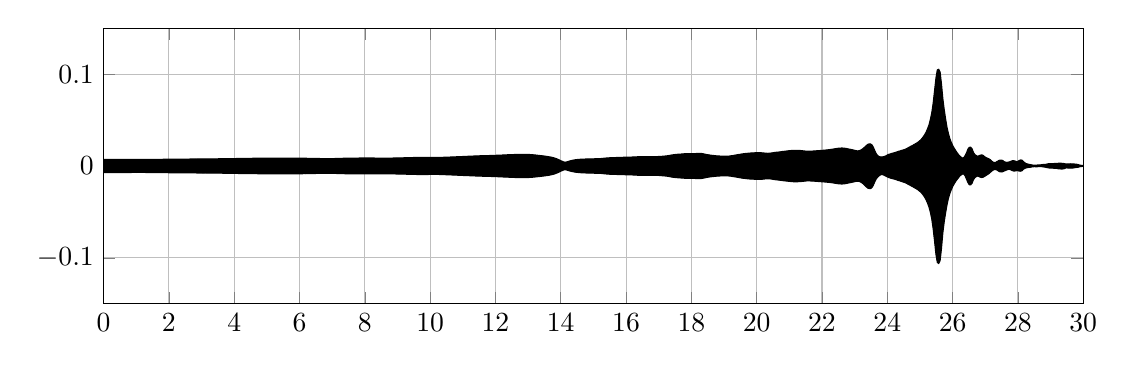
\begin{tikzpicture}

\begin{axis}[%
width=5.521in,
height=2in,
at={(0.758in,0.481in)},
xmin=0,
xmax=30,
xmajorgrids,
ymin=-0.15,
ymax=0.15,
ymajorgrids,
axis background/.style={fill=white}
]
\addplot[fill=black,draw=black,forget plot] plot table[row sep=crcr]{%
2.08333333333333e-05	0.00711667537689209\\
0.0425739952718676	0.00715172290802002\\
0.0851271572104019	0.00717854499816895\\
0.127680319148936	0.00717389583587646\\
0.17023348108747	0.00716269016265869\\
0.212786643026005	0.00716984272003174\\
0.255339804964539	0.00715470314025879\\
0.297892966903073	0.00717675685882568\\
0.340446128841608	0.00716102123260498\\
0.382999290780142	0.00713050365447998\\
0.425552452718676	0.00713396072387695\\
0.46810561465721	0.007110595703125\\
0.510658776595745	0.00710797309875488\\
0.553211938534279	0.00710749626159668\\
0.595765100472813	0.00713169574737549\\
0.638318262411347	0.00711977481842041\\
0.680871424349882	0.00706911087036133\\
0.723424586288416	0.00707662105560303\\
0.76597774822695	0.00704419612884521\\
0.808530910165485	0.00702989101409912\\
0.851084072104019	0.0070265531539917\\
0.893637234042553	0.00705957412719727\\
0.936190395981088	0.00704705715179443\\
0.978743557919622	0.00701904296875\\
1.02129671985816	0.00703704357147217\\
1.06384988179669	0.00701916217803955\\
1.10640304373522	0.00700545310974121\\
1.14895620567376	0.00700914859771729\\
1.19150936761229	0.00702071189880371\\
1.23406252955083	0.007010817527771\\
1.27661569148936	0.00704002380371094\\
1.3191688534279	0.00706374645233154\\
1.36172201536643	0.0070490837097168\\
1.40427517730496	0.00705838203430176\\
1.4468283392435	0.00709164142608643\\
1.48938150118203	0.00709640979766846\\
1.53193466312057	0.00711667537689209\\
1.5744878250591	0.00713801383972168\\
1.61704098699764	0.00712680816650391\\
1.65959414893617	0.00716006755828857\\
1.7021473108747	0.00717151165008545\\
1.74470047281324	0.00722146034240723\\
1.78725363475177	0.007224440574646\\
1.82980679669031	0.00726532936096191\\
1.87235995862884	0.00729167461395264\\
1.91491312056738	0.00730693340301514\\
1.95746628250591	0.00729870796203613\\
2.00001944444444	0.00730836391448975\\
2.04257260638298	0.00733256340026855\\
2.08512576832151	0.00735127925872803\\
2.12767893026005	0.00735330581665039\\
2.17023209219858	0.00736427307128906\\
2.21278525413712	0.00737285614013672\\
2.25533841607565	0.00740957260131836\\
2.29789157801418	0.0074305534362793\\
2.34044473995272	0.00741589069366455\\
2.38299790189125	0.0074392557144165\\
2.42555106382979	0.00744307041168213\\
2.46810422576832	0.00746047496795654\\
2.51065738770686	0.00747394561767578\\
2.55321054964539	0.00750064849853516\\
2.59576371158392	0.00749313831329346\\
2.63831687352246	0.00752484798431396\\
2.68087003546099	0.00753533840179443\\
2.72342319739953	0.00754857063293457\\
2.76597635933806	0.00754690170288086\\
2.8085295212766	0.00758397579193115\\
2.85108268321513	0.00756204128265381\\
2.89363584515366	0.00761198997497559\\
2.9361890070922	0.00759041309356689\\
2.97874216903073	0.00763452053070068\\
3.02129533096927	0.00764131546020508\\
3.0638484929078	0.00762450695037842\\
3.10640165484634	0.00765585899353027\\
3.14895481678487	0.00769960880279541\\
3.1915079787234	0.00766289234161377\\
3.23406114066194	0.00769424438476563\\
3.27661430260047	0.00768411159515381\\
3.31916746453901	0.00773382186889648\\
3.36172062647754	0.00774002075195313\\
3.40427378841608	0.00771880149841309\\
3.44682695035461	0.00775480270385742\\
3.48938011229314	0.00777649879455566\\
3.53193327423168	0.00781238079071045\\
3.57448643617021	0.00782144069671631\\
3.61703959810875	0.00782608985900879\\
3.65959276004728	0.00784993171691895\\
3.70214592198582	0.00787663459777832\\
3.74469908392435	0.00789356231689453\\
3.78725224586288	0.0079265832901001\\
3.82980540780142	0.00796341896057129\\
3.87235856973995	0.00796127319335938\\
3.91491173167849	0.00796675682067871\\
3.95746489361702	0.00801956653594971\\
4.00001805555556	0.00805056095123291\\
4.04257121749409	0.00805842876434326\\
4.08512437943262	0.00810146331787109\\
4.12767754137116	0.00813150405883789\\
4.17023070330969	0.00813031196594238\\
4.21278386524823	0.00816905498504639\\
4.25533702718676	0.00820612907409668\\
4.29789018912529	0.00819897651672363\\
4.34044335106383	0.00823402404785156\\
4.38299651300236	0.00826823711395264\\
4.4255496749409	0.00828671455383301\\
4.46810283687943	0.00829422473907471\\
4.51065599881797	0.00831139087677002\\
4.5532091607565	0.00833594799041748\\
4.59576232269503	0.00837421417236328\\
4.63831548463357	0.00838351249694824\\
4.6808686465721	0.00841653347015381\\
4.72342180851064	0.00843977928161621\\
4.76597497044917	0.00844264030456543\\
4.80852813238771	0.00843644142150879\\
4.85108129432624	0.00848281383514404\\
4.89363445626477	0.00847935676574707\\
4.93618761820331	0.00847780704498291\\
4.97874078014184	0.00851523876190186\\
5.02129394208038	0.00853025913238525\\
5.06384710401891	0.00852453708648682\\
5.10640026595745	0.00851666927337646\\
5.14895342789598	0.00854706764221191\\
5.19150658983452	0.00855875015258789\\
5.23405975177305	0.00856006145477295\\
5.27661291371158	0.00858712196350098\\
5.31916607565012	0.00855278968811035\\
5.36171923758865	0.00856626033782959\\
5.40427239952719	0.00858950614929199\\
5.44682556146572	0.00856506824493408\\
5.48937872340426	0.00856912136077881\\
5.53193188534279	0.0085984468460083\\
5.57448504728132	0.00858497619628906\\
5.61703820921986	0.00858128070831299\\
5.65959137115839	0.0085829496383667\\
5.70214453309693	0.00855660438537598\\
5.74469769503546	0.0085529088973999\\
5.787250856974	0.00854575634002686\\
5.82980401891253	0.00854003429412842\\
5.87235718085106	0.00852453708648682\\
5.9149103427896	0.00850319862365723\\
5.95746350472813	0.0084831714630127\\
6.00001666666667	0.00846600532531738\\
6.0425698286052	0.00844025611877441\\
6.08512299054374	0.00839424133300781\\
6.12767615248227	0.00841820240020752\\
6.1702293144208	0.0083698034286499\\
6.21278247635934	0.00835967063903809\\
6.25533563829787	0.0083012580871582\\
6.29788880023641	0.00829422473907471\\
6.34044196217494	0.00826966762542725\\
6.38299512411347	0.00821447372436523\\
6.42554828605201	0.00817787647247314\\
6.46810144799054	0.00813615322113037\\
6.51065460992908	0.00815653800964355\\
6.55320777186761	0.00810849666595459\\
6.59576093380615	0.00809025764465332\\
6.63831409574468	0.00805926322937012\\
6.68086725768321	0.0080108642578125\\
6.72342041962175	0.00798916816711426\\
6.76597358156028	0.00795292854309082\\
6.80852674349882	0.00798964500427246\\
6.85107990543735	0.00793993473052979\\
6.89363306737589	0.00796926021575928\\
6.93618622931442	0.00797343254089355\\
6.97873939125296	0.00799095630645752\\
7.02129255319149	0.00801503658294678\\
7.06384571513002	0.00806045532226563\\
7.10639887706856	0.00808882713317871\\
7.14895203900709	0.00812149047851563\\
7.19150520094563	0.00820076465606689\\
7.23405836288416	0.00824320316314697\\
7.27661152482269	0.00827836990356445\\
7.31916468676123	0.00833046436309814\\
7.36171784869976	0.00837016105651855\\
7.4042710106383	0.00839686393737793\\
7.44682417257683	0.00845658779144287\\
7.48937733451537	0.00846612453460693\\
7.5319304964539	0.00852656364440918\\
7.57448365839243	0.00851738452911377\\
7.61703682033097	0.00855374336242676\\
7.6595899822695	0.00855004787445068\\
7.70214314420804	0.00857579708099365\\
7.74469630614657	0.00859999656677246\\
7.78724946808511	0.00858581066131592\\
7.82980263002364	0.00861799716949463\\
7.87235579196217	0.00863790512084961\\
7.91490895390071	0.00864124298095703\\
7.95746211583924	0.00862336158752441\\
8.00001527777778	0.00863683223724365\\
8.04256843971631	0.00864839553833008\\
8.08512160165485	0.00863087177276611\\
8.12767476359338	0.00862336158752441\\
8.17022792553192	0.0086284875869751\\
8.21278108747045	0.00864791870117188\\
8.25533424940898	0.00863504409790039\\
8.29788741134752	0.00861430168151855\\
8.34044057328605	0.0085761547088623\\
8.38299373522459	0.00857341289520264\\
8.42554689716312	0.00858199596405029\\
8.46810005910165	0.00853908061981201\\
8.51065322104019	0.00851523876190186\\
8.55320638297872	0.00849854946136475\\
8.59575954491726	0.0084998607635498\\
8.63831270685579	0.00850272178649902\\
8.68086586879433	0.00852286815643311\\
8.72341903073286	0.00855743885040283\\
8.76597219267139	0.0085303783416748\\
8.80852535460993	0.00856375694274902\\
8.85107851654846	0.00860679149627686\\
8.893631678487	0.00864040851593018\\
8.93618484042553	0.00866103172302246\\
8.97873800236407	0.00870013236999512\\
9.0212911643026	0.00871646404266357\\
9.06384432624114	0.00875973701477051\\
9.10639748817967	0.00879406929016113\\
9.1489506501182	0.00882065296173096\\
9.19150381205674	0.00889372825622559\\
9.23405697399527	0.00892043113708496\\
9.27661013593381	0.00895595550537109\\
9.31916329787234	0.00901269912719727\\
9.36171645981088	0.00905239582061768\\
9.40426962174941	0.00907778739929199\\
9.44682278368794	0.00911951065063477\\
9.48937594562648	0.00916361808776855\\
9.53192910756501	0.00920963287353516\\
9.57448226950355	0.00924932956695557\\
9.61703543144208	0.00926709175109863\\
9.65958859338062	0.00924336910247803\\
9.70214175531915	0.00929093360900879\\
9.74469491725768	0.00930845737457275\\
9.78724807919622	0.00931012630462646\\
9.82980124113475	0.00931394100189209\\
9.87235440307329	0.00926542282104492\\
9.91490756501182	0.00927877426147461\\
9.95746072695036	0.00922882556915283\\
10.0000138888889	0.00920701026916504\\
10.0425670508274	0.00918543338775635\\
10.085120212766	0.00919544696807861\\
10.1276733747045	0.00918710231781006\\
10.170226536643	0.00920331478118896\\
10.2127796985816	0.00922286510467529\\
10.2553328605201	0.00926470756530762\\
10.2978860224586	0.00928342342376709\\
10.3404391843972	0.00933611392974854\\
10.3829923463357	0.00936532020568848\\
10.4255455082742	0.00948715209960938\\
10.4680986702128	0.00953006744384766\\
10.5106518321513	0.00956428050994873\\
10.5532049940898	0.00961589813232422\\
10.5957581560284	0.00968062877655029\\
10.6383113179669	0.00972402095794678\\
10.6808644799054	0.00978422164916992\\
10.723417641844	0.00985956192016602\\
10.7659708037825	0.00992977619171143\\
10.808523965721	0.00999200344085693\\
10.8510771276596	0.0100315809249878\\
10.8936302895981	0.0101125240325928\\
10.9361834515366	0.0101859569549561\\
10.9787366134752	0.0102301836013794\\
11.0212897754137	0.0103023052215576\\
11.0638429373522	0.0103899240493774\\
11.1063960992908	0.0104495286941528\\
11.1489492612293	0.0105196237564087\\
11.1915024231678	0.0105588436126709\\
11.2340555851064	0.0106586217880249\\
11.2766087470449	0.0107104778289795\\
11.3191619089835	0.0107804536819458\\
11.361715070922	0.0108331441879272\\
11.4042682328605	0.0109068155288696\\
11.4468213947991	0.0109307765960693\\
11.4893745567376	0.0110116004943848\\
11.5319277186761	0.0111005306243896\\
11.5744808806147	0.011115550994873\\
11.6170340425532	0.0111302137374878\\
11.6595872044917	0.0111647844314575\\
11.7021403664303	0.0112214088439941\\
11.7446935283688	0.0112656354904175\\
11.7872466903073	0.0113087892532349\\
11.8297998522459	0.0113542079925537\\
11.8723530141844	0.0113934278488159\\
11.9149061761229	0.0114550590515137\\
11.9574593380615	0.0114960670471191\\
12.0000125	0.0115586519241333\\
12.0425656619385	0.0116446018218994\\
12.0851188238771	0.0117003917694092\\
12.1276719858156	0.0117672681808472\\
12.1702251477541	0.0118402242660522\\
12.2127783096927	0.0118837356567383\\
12.2553314716312	0.0120162963867188\\
12.2978846335697	0.0120596885681152\\
12.3404377955083	0.0121123790740967\\
12.3829909574468	0.0121985673904419\\
12.4255441193853	0.0122308731079102\\
12.4680972813239	0.0122917890548706\\
12.5106504432624	0.0123668909072876\\
12.5532036052009	0.0124084949493408\\
12.5957567671395	0.0124773979187012\\
12.638309929078	0.0125191211700439\\
12.6808630910165	0.0125521421432495\\
12.7234162529551	0.0126339197158813\\
12.7659694148936	0.012651801109314\\
12.8085225768322	0.0126447677612305\\
12.8510757387707	0.0126558542251587\\
12.8936289007092	0.0126417875289917\\
12.9361820626478	0.0126105546951294\\
12.9787352245863	0.0125713348388672\\
13.0212883865248	0.012489914894104\\
13.0638415484634	0.012397289276123\\
13.1063947104019	0.0123105049133301\\
13.1489478723404	0.0121878385543823\\
13.191501034279	0.0120493173599243\\
13.2340541962175	0.0118894577026367\\
13.276607358156	0.0116817951202393\\
13.3191605200946	0.0115182399749756\\
13.3617136820331	0.0113525390625\\
13.4042668439716	0.0112044811248779\\
13.4468200059102	0.0110361576080322\\
13.4893731678487	0.0108188390731812\\
13.5319263297872	0.0106247663497925\\
13.5744794917258	0.0103753805160522\\
13.6170326536643	0.0101196765899658\\
13.6595858156028	0.00986087322235107\\
13.7021389775414	0.00961053371429443\\
13.7446921394799	0.0092613697052002\\
13.7872453014184	0.00886452198028564\\
13.829798463357	0.00836563110351563\\
13.8723516252955	0.00782811641693115\\
13.914904787234	0.00719857215881348\\
13.9574579491726	0.00650393962860107\\
14.0000111111111	0.00577068328857422\\
14.0425642730496	0.00507986545562744\\
14.0851174349882	0.00443530082702637\\
14.1276705969267	0.0040738582611084\\
14.1702237588652	0.0043034553527832\\
14.2127769208038	0.00470757484436035\\
14.2553300827423	0.00520455837249756\\
14.2978832446809	0.00561857223510742\\
14.3404364066194	0.00600862503051758\\
14.3829895685579	0.00633060932159424\\
14.4255427304965	0.00659990310668945\\
14.468095892435	0.00683057308197021\\
14.5106490543735	0.00700163841247559\\
14.5532022163121	0.00716352462768555\\
14.5957553782506	0.00726437568664551\\
14.6383085401891	0.00736451148986816\\
14.6808617021277	0.00744724273681641\\
14.7234148640662	0.00749886035919189\\
14.7659680260047	0.00753605365753174\\
14.8085211879433	0.00760531425476074\\
14.8510743498818	0.00765800476074219\\
14.8936275118203	0.00770962238311768\\
14.9361806737589	0.00772929191589355\\
14.9787338356974	0.00777053833007813\\
15.0212869976359	0.00778889656066895\\
15.0638401595745	0.00782406330108643\\
15.106393321513	0.00786161422729492\\
15.1489464834515	0.00791490077972412\\
15.1914996453901	0.00798928737640381\\
15.2340528073286	0.00808358192443848\\
15.2766059692671	0.00822067260742188\\
15.3191591312057	0.00838017463684082\\
15.3617122931442	0.00854873657226563\\
15.4042654550827	0.0086592435836792\\
15.4468186170213	0.0087820291519165\\
15.4893717789598	0.00888705253601074\\
15.5319249408983	0.00896096229553223\\
15.5744781028369	0.00902485847473145\\
15.6170312647754	0.00909948348999023\\
15.6595844267139	0.00911784172058105\\
15.7021375886525	0.00916874408721924\\
15.744690750591	0.00925087928771973\\
15.7872439125296	0.00928473472595215\\
15.8297970744681	0.0093226432800293\\
15.8723502364066	0.009368896484375\\
15.9149033983452	0.00944066047668457\\
15.9574565602837	0.00946617126464844\\
16.0000097222222	0.00950753688812256\\
16.0425628841608	0.00956380367279053\\
16.0851160460993	0.00956130027770996\\
16.1276692080378	0.0096285343170166\\
16.1702223699764	0.00967848300933838\\
16.2127755319149	0.00976920127868652\\
16.2553286938534	0.0098346471786499\\
16.297881855792	0.00993049144744873\\
16.3404350177305	0.00997734069824219\\
16.382988179669	0.0100448131561279\\
16.4255413416076	0.0101383924484253\\
16.4680945035461	0.010167121887207\\
16.5106476654846	0.0101839303970337\\
16.5532008274232	0.0101522207260132\\
16.5957539893617	0.0101271867752075\\
16.6383071513002	0.0100888013839722\\
16.6808603132388	0.010079026222229\\
16.7234134751773	0.0100340843200684\\
16.7659666371158	0.0100160837173462\\
16.8085197990544	0.0100369453430176\\
16.8510729609929	0.0100862979888916\\
16.8936261229314	0.0101287364959717\\
16.93617928487	0.0101354122161865\\
16.9787324468085	0.0102592706680298\\
17.021285608747	0.0103194713592529\\
17.0638387706856	0.0103678703308105\\
17.1063919326241	0.0105175971984863\\
17.1489450945626	0.0106227397918701\\
17.1914982565012	0.0107946395874023\\
17.2340514184397	0.0109468698501587\\
17.2766045803783	0.0111522674560547\\
17.3191577423168	0.01143479347229\\
17.3617109042553	0.0116888284683228\\
17.4042640661939	0.0119591951370239\\
17.4468172281324	0.0121793746948242\\
17.4893703900709	0.0123839378356934\\
17.5319235520095	0.0125503540039063\\
17.574476713948	0.0127048492431641\\
17.6170298758865	0.0128219127655029\\
17.6595830378251	0.0128920078277588\\
17.7021361997636	0.0130268335342407\\
17.7446893617021	0.0131461620330811\\
17.7872425236407	0.013282299041748\\
17.8297956855792	0.0133534669876099\\
17.8723488475177	0.0134086608886719\\
17.9149020094563	0.0134586095809937\\
17.9574551713948	0.0134837627410889\\
18.0000083333333	0.0134778022766113\\
18.0425614952719	0.0134320259094238\\
18.0851146572104	0.0133986473083496\\
18.1276678191489	0.0134919881820679\\
18.1702209810875	0.0135809183120728\\
18.212774143026	0.0136455297470093\\
18.2553273049645	0.0136773586273193\\
18.2978804669031	0.0135959386825562\\
18.3404336288416	0.0134341716766357\\
18.3829867907801	0.0131129026412964\\
18.4255399527187	0.0127367973327637\\
18.4680931146572	0.012428879737854\\
18.5106462765957	0.0121810436248779\\
18.5531994385343	0.0119520425796509\\
18.5957526004728	0.0117126703262329\\
18.6383057624113	0.0115468502044678\\
18.6808589243499	0.0113520622253418\\
18.7234120862884	0.011198878288269\\
18.765965248227	0.0110090970993042\\
18.8085184101655	0.0109310150146484\\
18.851071572104	0.0108126401901245\\
18.8936247340426	0.0107583999633789\\
18.9361778959811	0.0106978416442871\\
18.9787310579196	0.0106565952301025\\
19.0212842198582	0.0106431245803833\\
19.0638373817967	0.0105493068695068\\
19.1063905437352	0.0105994939804077\\
19.1489437056738	0.0107020139694214\\
19.1914968676123	0.0109293460845947\\
19.2340500295508	0.0111761093139648\\
19.2766031914894	0.0113557577133179\\
19.3191563534279	0.0116512775421143\\
19.3617095153664	0.0119069814682007\\
19.404262677305	0.0122066736221313\\
19.4468158392435	0.0124557018280029\\
19.489369001182	0.0126534700393677\\
19.5319221631206	0.0129510164260864\\
19.5744753250591	0.0131763219833374\\
19.6170284869976	0.0134081840515137\\
19.6595816489362	0.0135430097579956\\
19.7021348108747	0.0137039422988892\\
19.7446879728132	0.0138463973999023\\
19.7872411347518	0.0139881372451782\\
19.8297942966903	0.0141350030899048\\
19.8723474586288	0.0142196416854858\\
19.9149006205674	0.0142802000045776\\
19.9574537825059	0.014367938041687\\
20.0000069444444	0.014385461807251\\
20.042560106383	0.0144249200820923\\
20.0851132683215	0.0144028663635254\\
20.12766643026	0.0143833160400391\\
20.1702195921986	0.0142660140991211\\
20.2127727541371	0.0141717195510864\\
20.2553259160756	0.0139555931091309\\
20.2978790780142	0.0138499736785889\\
20.3404322399527	0.0137612819671631\\
20.3829854018913	0.0138204097747803\\
20.4255385638298	0.0139924287796021\\
20.4680917257683	0.0141996145248413\\
20.5106448877069	0.0144475698471069\\
20.5531980496454	0.0146808624267578\\
20.5957512115839	0.0148940086364746\\
20.6383043735225	0.015020489692688\\
20.680857535461	0.0151877403259277\\
20.7234106973995	0.0153675079345703\\
20.7659638593381	0.0155923366546631\\
20.8085170212766	0.0158268213272095\\
20.8510701832151	0.0159734487533569\\
20.8936233451537	0.016166090965271\\
20.9361765070922	0.0163371562957764\\
20.9787296690307	0.0165252685546875\\
21.0212828309693	0.0166422128677368\\
21.0638359929078	0.0168395042419434\\
21.1063891548463	0.0168962478637695\\
21.1489423167849	0.01697838306427\\
21.1914954787234	0.0170114040374756\\
21.2340486406619	0.0170043706893921\\
21.2766018026005	0.0169713497161865\\
21.319154964539	0.016831636428833\\
21.3617081264775	0.0167328119277954\\
21.4042612884161	0.0165444612503052\\
21.4468144503546	0.0163892507553101\\
21.4893676122931	0.0162161588668823\\
21.5319207742317	0.0161160230636597\\
21.5744739361702	0.0160380601882935\\
21.6170270981087	0.0160644054412842\\
21.6595802600473	0.0160897970199585\\
21.7021334219858	0.0161862373352051\\
21.7446865839243	0.0162837505340576\\
21.7872397458629	0.016431450843811\\
21.8297929078014	0.0165103673934937\\
21.87234606974	0.0166468620300293\\
21.9148992316785	0.0167297124862671\\
21.957452393617	0.016843318939209\\
22.0000055555556	0.0169404745101929\\
22.0425587174941	0.017126202583313\\
22.0851118794326	0.0172253847122192\\
22.1276650413712	0.0173736810684204\\
22.1702182033097	0.0175583362579346\\
22.2127713652482	0.0177210569381714\\
22.2553245271868	0.0179535150527954\\
22.2978776891253	0.0181349515914917\\
22.3404308510638	0.0183558464050293\\
22.3829840130024	0.0186412334442139\\
22.4255371749409	0.0188684463500977\\
22.4680903368794	0.0191171169281006\\
22.510643498818	0.019382119178772\\
22.5531966607565	0.0194610357284546\\
22.595749822695	0.0195201635360718\\
22.6383029846336	0.0194985866546631\\
22.6808561465721	0.0193488597869873\\
22.7234093085106	0.0191479921340942\\
22.7659624704492	0.0188283920288086\\
22.8085156323877	0.0184992551803589\\
22.8510687943262	0.0182352066040039\\
22.8936219562648	0.0179296731948853\\
22.9361751182033	0.0175976753234863\\
22.9787282801418	0.0172501802444458\\
23.0212814420804	0.0168391466140747\\
23.0638346040189	0.0165137052536011\\
23.1063877659574	0.0164340734481812\\
23.148940927896	0.0167514085769653\\
23.1914940898345	0.0174319744110107\\
23.234047251773	0.0183174610137939\\
23.2766004137116	0.0194990634918213\\
23.3191535756501	0.020859956741333\\
23.3617067375887	0.0223097801208496\\
23.4042598995272	0.0235520601272583\\
23.4468130614657	0.0240000486373901\\
23.4893662234043	0.023932933807373\\
23.5319193853428	0.0228255987167358\\
23.5744725472813	0.020297646522522\\
23.6170257092199	0.0166084766387939\\
23.6595788711584	0.0134152173995972\\
23.7021320330969	0.0113495588302612\\
23.7446851950355	0.0103473663330078\\
23.787238356974	0.0098642110824585\\
23.8297915189125	0.00985598564147949\\
23.8723446808511	0.00998532772064209\\
23.9148978427896	0.0103533267974854\\
23.9574510047281	0.0110429525375366\\
24.0000041666667	0.0118612051010132\\
24.0425573286052	0.0126634836196899\\
24.0851104905437	0.013016939163208\\
24.1276636524823	0.0135705471038818\\
24.1702168144208	0.0139542818069458\\
24.2127699763593	0.0143481492996216\\
24.2553231382979	0.0148164033889771\\
24.2978763002364	0.0153217315673828\\
24.3404294621749	0.0159354209899902\\
24.3829826241135	0.0162891149520874\\
24.425535786052	0.0168496370315552\\
24.4680889479905	0.0172262191772461\\
24.5106421099291	0.0177273750305176\\
24.5531952718676	0.0181947946548462\\
24.5957484338061	0.0188931226730347\\
24.6383015957447	0.0198160409927368\\
24.6808547576832	0.0206384658813477\\
24.7234079196217	0.0214669704437256\\
24.7659610815603	0.0221570730209351\\
24.8085142434988	0.023077130317688\\
24.8510674054374	0.0239729881286621\\
24.8936205673759	0.0247877836227417\\
24.9361737293144	0.0257978439331055\\
24.978726891253	0.0270137786865234\\
25.0212800531915	0.0282821655273438\\
25.06383321513	0.0299826860427856\\
25.1063863770686	0.0320037603378296\\
25.1489395390071	0.034333348274231\\
25.1914927009456	0.0370622873306274\\
25.2340458628842	0.0407503843307495\\
25.2765990248227	0.0447026491165161\\
25.3191521867612	0.0505886077880859\\
25.3617053486998	0.0579507350921631\\
25.4042585106383	0.0683985948562622\\
25.4468116725768	0.0818861722946167\\
25.4893648345154	0.0956288576126099\\
25.5319179964539	0.104615211486816\\
25.5744711583924	0.105268955230713\\
25.617024320331	0.102339625358582\\
25.6595774822695	0.0891133546829224\\
25.702130644208	0.0730127096176147\\
25.7446838061466	0.060924768447876\\
25.7872369680851	0.0509119033813477\\
25.8297901300236	0.0417578220367432\\
25.8723432919622	0.0352636575698853\\
25.9148964539007	0.0297328233718872\\
25.9574496158392	0.0258671045303345\\
26.0000027777778	0.0224037170410156\\
26.0425559397163	0.0197221040725708\\
26.0851091016548	0.0172529220581055\\
26.1276622635934	0.0149737596511841\\
26.1702154255319	0.0128642320632935\\
26.2127685874705	0.0110783576965332\\
26.255321749409	0.00973069667816162\\
26.2978749113475	0.00867378711700439\\
26.3404280732861	0.00899934768676758\\
26.3829812352246	0.0111793279647827\\
26.4255343971631	0.0142389535903931\\
26.4680875591017	0.0182769298553467\\
26.5106407210402	0.0202749967575073\\
26.5531938829787	0.0204064846038818\\
26.5957470449173	0.0186686515808105\\
26.6383002068558	0.0146009922027588\\
26.6808533687943	0.0124722719192505\\
26.7234065307329	0.0112890005111694\\
26.7659596926714	0.0106105804443359\\
26.8085128546099	0.0110818147659302\\
26.8510660165485	0.0117746591567993\\
26.893619178487	0.012041449546814\\
26.9361723404255	0.011481761932373\\
26.9787255023641	0.0101684331893921\\
27.0212786643026	0.00910913944244385\\
27.0638318262411	0.00849020481109619\\
27.1063849881797	0.00777816772460938\\
27.1489381501182	0.00695478916168213\\
27.1914913120567	0.00548660755157471\\
27.2340444739953	0.00421905517578125\\
27.2765976359338	0.00375306606292725\\
27.3191507978723	0.00399541854858398\\
27.3617039598109	0.00479984283447266\\
27.4042571217494	0.00570535659790039\\
27.4468102836879	0.00640738010406494\\
27.4893634456265	0.00638580322265625\\
27.531916607565	0.00599193572998047\\
27.5744697695035	0.00473988056182861\\
27.6170229314421	0.00419318675994873\\
27.6595760933806	0.00389528274536133\\
27.7021292553192	0.00410258769989014\\
27.7446824172577	0.00450479984283447\\
27.7872355791962	0.0050894021987915\\
27.8297887411348	0.00568115711212158\\
27.8723419030733	0.00572729110717773\\
27.9148950650118	0.00529897212982178\\
27.9574482269504	0.0047067403793335\\
28.0000013888889	0.00500047206878662\\
28.0425545508274	0.00604903697967529\\
28.085107712766	0.00651252269744873\\
28.1276608747045	0.00630855560302734\\
28.170214036643	0.00482082366943359\\
28.2127671985816	0.00334036350250244\\
28.2553203605201	0.00249338150024414\\
28.2978735224586	0.00213503837585449\\
28.3404266843972	0.00172114372253418\\
28.3829798463357	0.00145041942596436\\
28.4255330082742	0.00112783908843994\\
28.4680861702128	0.000860691070556641\\
28.5106393321513	0.000752687454223633\\
28.5531924940898	0.000847101211547852\\
28.5957456560284	0.00100839138031006\\
28.6382988179669	0.00103020668029785\\
28.6808519799054	0.00108325481414795\\
28.723405141844	0.00141811370849609\\
28.7659583037825	0.00156378746032715\\
28.808511465721	0.001639723777771\\
28.8510646276596	0.00171160697937012\\
28.8936177895981	0.00209367275238037\\
28.9361709515366	0.00239336490631104\\
28.9787241134752	0.00247716903686523\\
29.0212772754137	0.00249373912811279\\
29.0638304373522	0.00254380702972412\\
29.1063835992908	0.00264203548431396\\
29.1489367612293	0.0027540922164917\\
29.1914899231679	0.0028538703918457\\
29.2340430851064	0.00289309024810791\\
29.2765962470449	0.00299191474914551\\
29.3191494089835	0.00294983386993408\\
29.361702570922	0.00278544425964355\\
29.4042557328605	0.00262033939361572\\
29.4468088947991	0.00233495235443115\\
29.4893620567376	0.00202608108520508\\
29.5319152186761	0.00233829021453857\\
29.5744683806147	0.00221478939056396\\
29.6170215425532	0.00236570835113525\\
29.6595747044917	0.00222063064575195\\
29.7021278664303	0.00224399566650391\\
29.7446810283688	0.00204455852508545\\
29.7872341903073	0.00188469886779785\\
29.8297873522459	0.00169014930725098\\
29.8723405141844	0.00110828876495361\\
29.9148936761229	0.000838637351989746\\
29.9574468380615	0.000568270683288574\\
30	0.000414729118347168\\
}
\closedcycle;
\addplot[fill=black,draw=black,forget plot] plot table[row sep=crcr]{%
2.08333333333333e-05	-0.00716090202331543\\
0.0425739952718676	-0.00717389583587646\\
0.0851271572104019	-0.00717127323150635\\
0.127680319148936	-0.00721180438995361\\
0.17023348108747	-0.00718295574188232\\
0.212786643026005	-0.00718975067138672\\
0.255339804964539	-0.00718879699707031\\
0.297892966903073	-0.00717556476593018\\
0.340446128841608	-0.00715541839599609\\
0.382999290780142	-0.00715172290802002\\
0.425552452718676	-0.00715339183807373\\
0.46810561465721	-0.00712752342224121\\
0.510658776595745	-0.00713932514190674\\
0.553211938534279	-0.00711452960968018\\
0.595765100472813	-0.00710546970367432\\
0.638318262411347	-0.00707697868347168\\
0.680871424349882	-0.00710666179656982\\
0.723424586288416	-0.00708699226379395\\
0.76597774822695	-0.00707614421844482\\
0.808530910165485	-0.00706124305725098\\
0.851084072104019	-0.00707197189331055\\
0.893637234042553	-0.00702857971191406\\
0.936190395981088	-0.0070265531539917\\
0.978743557919622	-0.00705873966217041\\
1.02129671985816	-0.00706326961517334\\
1.06384988179669	-0.00702357292175293\\
1.10640304373522	-0.00703787803649902\\
1.14895620567376	-0.0070490837097168\\
1.19150936761229	-0.00704169273376465\\
1.23406252955083	-0.0070500373840332\\
1.27661569148936	-0.00706124305725098\\
1.3191688534279	-0.00708913803100586\\
1.36172201536643	-0.0070720911026001\\
1.40427517730496	-0.00710546970367432\\
1.4468283392435	-0.00708544254302979\\
1.48938150118203	-0.00713169574737549\\
1.53193466312057	-0.00713133811950684\\
1.5744878250591	-0.00716972351074219\\
1.61704098699764	-0.00717794895172119\\
1.65959414893617	-0.00719344615936279\\
1.7021473108747	-0.00719928741455078\\
1.74470047281324	-0.00722110271453857\\
1.78725363475177	-0.00724387168884277\\
1.82980679669031	-0.00724303722381592\\
1.87235995862884	-0.00726735591888428\\
1.91491312056738	-0.00727534294128418\\
1.95746628250591	-0.00728392601013184\\
2.00001944444444	-0.00735878944396973\\
2.04257260638298	-0.00735032558441162\\
2.08512576832151	-0.00736749172210693\\
2.12767893026005	-0.00736463069915771\\
2.17023209219858	-0.0074237585067749\\
2.21278525413712	-0.00740325450897217\\
2.25533841607565	-0.00741243362426758\\
2.29789157801418	-0.00743496417999268\\
2.34044473995272	-0.00743556022644043\\
2.38299790189125	-0.00747096538543701\\
2.42555106382979	-0.00750887393951416\\
2.46810422576832	-0.00749385356903076\\
2.51065738770686	-0.00749433040618896\\
2.55321054964539	-0.00750815868377686\\
2.59576371158392	-0.0075535774230957\\
2.63831687352246	-0.00755929946899414\\
2.68087003546099	-0.00753939151763916\\
2.72342319739953	-0.00756561756134033\\
2.76597635933806	-0.00756931304931641\\
2.8085295212766	-0.00757348537445068\\
2.85108268321513	-0.00761747360229492\\
2.89363584515366	-0.00761198997497559\\
2.9361890070922	-0.00761699676513672\\
2.97874216903073	-0.00764036178588867\\
3.02129533096927	-0.00766777992248535\\
3.0638484929078	-0.00767612457275391\\
3.10640165484634	-0.00766170024871826\\
3.14895481678487	-0.00766658782958984\\
3.1915079787234	-0.00770127773284912\\
3.23406114066194	-0.00768923759460449\\
3.27661430260047	-0.00771081447601318\\
3.31916746453901	-0.00773751735687256\\
3.36172062647754	-0.00774300098419189\\
3.40427378841608	-0.00778758525848389\\
3.44682695035461	-0.00777387619018555\\
3.48938011229314	-0.00777876377105713\\
3.53193327423168	-0.00781047344207764\\
3.57448643617021	-0.00783944129943848\\
3.61703959810875	-0.00785815715789795\\
3.65959276004728	-0.00790441036224365\\
3.70214592198582	-0.0079503059387207\\
3.74469908392435	-0.00795149803161621\\
3.78725224586288	-0.0079571008682251\\
3.82980540780142	-0.00801217555999756\\
3.87235856973995	-0.00802624225616455\\
3.91491173167849	-0.00803792476654053\\
3.95746489361702	-0.00805675983428955\\
4.00001805555556	-0.0080639123916626\\
4.04257121749409	-0.00809395313262939\\
4.08512437943262	-0.0081101655960083\\
4.12767754137116	-0.00816309452056885\\
4.17023070330969	-0.00815927982330322\\
4.21278386524823	-0.00819098949432373\\
4.25533702718676	-0.00818228721618652\\
4.29789018912529	-0.00822532176971436\\
4.34044335106383	-0.00825023651123047\\
4.38299651300236	-0.00826025009155273\\
4.4255496749409	-0.00833046436309814\\
4.46810283687943	-0.00833547115325928\\
4.51065599881797	-0.00832831859588623\\
4.5532091607565	-0.00837600231170654\\
4.59576232269503	-0.00839102268218994\\
4.63831548463357	-0.0083850622177124\\
4.6808686465721	-0.00841474533081055\\
4.72342180851064	-0.00842809677124023\\
4.76597497044917	-0.00842761993408203\\
4.80852813238771	-0.00845479965209961\\
4.85108129432624	-0.00847065448760986\\
4.89363445626477	-0.00847434997558594\\
4.93618761820331	-0.00852453708648682\\
4.97874078014184	-0.00852859020233154\\
5.02129394208038	-0.00856781005859375\\
5.06384710401891	-0.00856697559356689\\
5.10640026595745	-0.00855028629302979\\
5.14895342789598	-0.008575439453125\\
5.19150658983452	-0.00857734680175781\\
5.23405975177305	-0.00857400894165039\\
5.27661291371158	-0.00857114791870117\\
5.31916607565012	-0.00860738754272461\\
5.36171923758865	-0.00862634181976318\\
5.40427239952719	-0.00859570503234863\\
5.44682556146572	-0.00863635540008545\\
5.48937872340426	-0.00862491130828857\\
5.53193188534279	-0.00863838195800781\\
5.57448504728132	-0.00860285758972168\\
5.61703820921986	-0.00860905647277832\\
5.65959137115839	-0.00857579708099365\\
5.70214453309693	-0.00860238075256348\\
5.74469769503546	-0.00857448577880859\\
5.787250856974	-0.00857579708099365\\
5.82980401891253	-0.00857400894165039\\
5.87235718085106	-0.0085594654083252\\
5.9149103427896	-0.00852775573730469\\
5.95746350472813	-0.00848782062530518\\
6.00001666666667	-0.00848114490509033\\
6.0425698286052	-0.00847733020782471\\
6.08512299054374	-0.00844430923461914\\
6.12767615248227	-0.00839436054229736\\
6.1702293144208	-0.00842523574829102\\
6.21278247635934	-0.00836920738220215\\
6.25533563829787	-0.00836098194122314\\
6.29788880023641	-0.00835263729095459\\
6.34044196217494	-0.00830113887786865\\
6.38299512411347	-0.00827085971832275\\
6.42554828605201	-0.00824415683746338\\
6.46810144799054	-0.00819242000579834\\
6.51065460992908	-0.00814223289489746\\
6.55320777186761	-0.00815010070800781\\
6.59576093380615	-0.0081181526184082\\
6.63831409574468	-0.00807750225067139\\
6.68086725768321	-0.00805509090423584\\
6.72342041962175	-0.00803422927856445\\
6.76597358156028	-0.00803256034851074\\
6.80852674349882	-0.00799071788787842\\
6.85107990543735	-0.00801002979278564\\
6.89363306737589	-0.00798463821411133\\
6.93618622931442	-0.00801205635070801\\
6.97873939125296	-0.00805377960205078\\
7.02129255319149	-0.00805807113647461\\
7.06384571513002	-0.00811183452606201\\
7.10639887706856	-0.00812804698944092\\
7.14895203900709	-0.00816726684570313\\
7.19150520094563	-0.00822830200195313\\
7.23405836288416	-0.00825238227844238\\
7.27661152482269	-0.00830924510955811\\
7.31916468676123	-0.00835037231445313\\
7.36171784869976	-0.00840389728546143\\
7.4042710106383	-0.00845110416412354\\
7.44682417257683	-0.00848734378814697\\
7.48937733451537	-0.00853872299194336\\
7.5319304964539	-0.00854957103729248\\
7.57448365839243	-0.00857532024383545\\
7.61703682033097	-0.00862133502960205\\
7.6595899822695	-0.00859701633453369\\
7.70214314420804	-0.00862669944763184\\
7.74469630614657	-0.00865054130554199\\
7.78724946808511	-0.00863170623779297\\
7.82980263002364	-0.00863873958587646\\
7.87235579196217	-0.0086524486541748\\
7.91490895390071	-0.00865292549133301\\
7.95746211583924	-0.00867307186126709\\
8.00001527777778	-0.00866913795471191\\
8.04256843971631	-0.00869560241699219\\
8.08512160165485	-0.00866460800170898\\
8.12767476359338	-0.00867879390716553\\
8.17022792553192	-0.00865793228149414\\
8.21278108747045	-0.00865375995635986\\
8.25533424940898	-0.00865256786346436\\
8.29788741134752	-0.00866842269897461\\
8.34044057328605	-0.00861704349517822\\
8.38299373522459	-0.00862205028533936\\
8.42554689716312	-0.00860238075256348\\
8.46810005910165	-0.0085906982421875\\
8.51065322104019	-0.00859618186950684\\
8.55320638297872	-0.00853443145751953\\
8.59575954491726	-0.00856709480285645\\
8.63831270685579	-0.0085529088973999\\
8.68086586879433	-0.00855040550231934\\
8.72341903073286	-0.00860130786895752\\
8.76597219267139	-0.0085911750793457\\
8.80852535460993	-0.00862789154052734\\
8.85107851654846	-0.00864970684051514\\
8.893631678487	-0.00864911079406738\\
8.93618484042553	-0.00868713855743408\\
8.97873800236407	-0.00872719287872314\\
9.0212911643026	-0.00876021385192871\\
9.06384432624114	-0.00879395008087158\\
9.10639748817967	-0.00882697105407715\\
9.1489506501182	-0.00885319709777832\\
9.19150381205674	-0.00888955593109131\\
9.23405697399527	-0.0089346170425415\\
9.27661013593381	-0.00897717475891113\\
9.31916329787234	-0.00902342796325684\\
9.36171645981088	-0.00906062126159668\\
9.40426962174941	-0.00909686088562012\\
9.44682278368794	-0.00915729999542236\\
9.48937594562648	-0.00916373729705811\\
9.53192910756501	-0.00922989845275879\\
9.57448226950355	-0.00923502445220947\\
9.61703543144208	-0.00928628444671631\\
9.65958859338062	-0.00927257537841797\\
9.70214175531915	-0.0093071460723877\\
9.74469491725768	-0.00932252407073975\\
9.78724807919622	-0.00931477546691895\\
9.82980124113475	-0.00932598114013672\\
9.87235440307329	-0.00931632518768311\\
9.91490756501182	-0.0092933177947998\\
9.95746072695036	-0.00923502445220947\\
10.0000138888889	-0.00924217700958252\\
10.0425670508274	-0.00918030738830566\\
10.085120212766	-0.0091547966003418\\
10.1276733747045	-0.00916481018066406\\
10.170226536643	-0.00919461250305176\\
10.2127796985816	-0.00920414924621582\\
10.2553328605201	-0.00922155380249023\\
10.2978860224586	-0.0092620849609375\\
10.3404391843972	-0.00932562351226807\\
10.3829923463357	-0.00939071178436279\\
10.4255455082742	-0.00945901870727539\\
10.4680986702128	-0.00950026512145996\\
10.5106518321513	-0.00956261157989502\\
10.5532049940898	-0.009621262550354\\
10.5957581560284	-0.00968694686889648\\
10.6383113179669	-0.00975525379180908\\
10.6808644799054	-0.00982630252838135\\
10.723417641844	-0.0098578929901123\\
10.7659708037825	-0.00994300842285156\\
10.808523965721	-0.0100101232528687\\
10.8510771276596	-0.0100923776626587\\
10.8936302895981	-0.0101537704467773\\
10.9361834515366	-0.0102071762084961\\
10.9787366134752	-0.0102885961532593\\
11.0212897754137	-0.0103439092636108\\
11.0638429373522	-0.0104503631591797\\
11.1063960992908	-0.0104997158050537\\
11.1489492612293	-0.0105371475219727\\
11.1915024231678	-0.0105859041213989\\
11.2340555851064	-0.0106768608093262\\
11.2766087470449	-0.0107487440109253\\
11.3191619089835	-0.0107853412628174\\
11.361715070922	-0.0108463764190674\\
11.4042682328605	-0.0109081268310547\\
11.4468213947991	-0.0109573602676392\\
11.4893745567376	-0.0110411643981934\\
11.5319277186761	-0.011104941368103\\
11.5744808806147	-0.0111179351806641\\
11.6170340425532	-0.0112018585205078\\
11.6595872044917	-0.011228084564209\\
11.7021403664303	-0.0112694501876831\\
11.7446935283688	-0.0112999677658081\\
11.7872466903073	-0.0113444328308105\\
11.8297998522459	-0.011408805847168\\
11.8723530141844	-0.0114213228225708\\
11.9149061761229	-0.0114587545394897\\
11.9574593380615	-0.0115351676940918\\
12.0000125	-0.0116169452667236\\
12.0425656619385	-0.011661171913147\\
12.0851188238771	-0.0117120742797852\\
12.1276719858156	-0.0118018388748169\\
12.1702251477541	-0.0118777751922607\\
12.2127783096927	-0.011944055557251\\
12.2553314716312	-0.0119959115982056\\
12.2978846335697	-0.0120670795440674\\
12.3404377955083	-0.0121381282806396\\
12.3829909574468	-0.0122014284133911\\
12.4255441193853	-0.012284517288208\\
12.4680972813239	-0.0123350620269775\\
12.5106504432624	-0.0124000310897827\\
12.5532036052009	-0.0124468803405762\\
12.5957567671395	-0.0125257968902588\\
12.638309929078	-0.0125710964202881\\
12.6808630910165	-0.0125865936279297\\
12.7234162529551	-0.0126174688339233\\
12.7659694148936	-0.0126612186431885\\
12.8085225768322	-0.0126837491989136\\
12.8510757387707	-0.0126951932907104\\
12.8936289007092	-0.0126618146896362\\
12.9361820626478	-0.0126467943191528\\
12.9787352245863	-0.0125794410705566\\
13.0212883865248	-0.0125575065612793\\
13.0638415484634	-0.012434720993042\\
13.1063947104019	-0.01233971118927\\
13.1489478723404	-0.0122290849685669\\
13.191501034279	-0.012049674987793\\
13.2340541962175	-0.0119369029998779\\
13.276607358156	-0.0117325782775879\\
13.3191605200946	-0.01160728931427\\
13.3617136820331	-0.0114662647247314\\
13.4042668439716	-0.0112539529800415\\
13.4468200059102	-0.0110625028610229\\
13.4893731678487	-0.0108667612075806\\
13.5319263297872	-0.0106652975082397\\
13.5744794917258	-0.0104274749755859\\
13.6170326536643	-0.0102634429931641\\
13.6595858156028	-0.00996971130371094\\
13.7021389775414	-0.00964689254760742\\
13.7446921394799	-0.0093076229095459\\
13.7872453014184	-0.00892496109008789\\
13.829798463357	-0.00840854644775391\\
13.8723516252955	-0.00779223442077637\\
13.914904787234	-0.00720429420471191\\
13.9574579491726	-0.00652134418487549\\
14.0000111111111	-0.00572490692138672\\
14.0425642730496	-0.00504219532012939\\
14.0851174349882	-0.00439178943634033\\
14.1276705969267	-0.00409126281738281\\
14.1702237588652	-0.00432240962982178\\
14.2127769208038	-0.00476276874542236\\
14.2553300827423	-0.00523793697357178\\
14.2978832446809	-0.00566005706787109\\
14.3404364066194	-0.00605559349060059\\
14.3829895685579	-0.00633406639099121\\
14.4255427304965	-0.00659346580505371\\
14.468095892435	-0.00685632228851318\\
14.5106490543735	-0.00700163841247559\\
14.5532022163121	-0.00720357894897461\\
14.5957553782506	-0.00730621814727783\\
14.6383085401891	-0.00740242004394531\\
14.6808617021277	-0.00747668743133545\\
14.7234148640662	-0.00756180286407471\\
14.7659680260047	-0.00760948657989502\\
14.8085211879433	-0.00764751434326172\\
14.8510743498818	-0.00769829750061035\\
14.8936275118203	-0.00773251056671143\\
14.9361806737589	-0.00779426097869873\\
14.9787338356974	-0.00782310962677002\\
15.0212869976359	-0.00788199901580811\\
15.0638401595745	-0.00789618492126465\\
15.106393321513	-0.00791740417480469\\
15.1489464834515	-0.00795543193817139\\
15.1914996453901	-0.00803971290588379\\
15.2340528073286	-0.00810635089874268\\
15.2766059692671	-0.00825190544128418\\
15.3191591312057	-0.00843441486358643\\
15.3617122931442	-0.00860202312469482\\
15.4042654550827	-0.00873315334320068\\
15.4468186170213	-0.00888276100158691\\
15.4893717789598	-0.00896632671356201\\
15.5319249408983	-0.00903213024139404\\
15.5744781028369	-0.00908350944519043\\
15.6170312647754	-0.0091170072555542\\
15.6595844267139	-0.00918865203857422\\
15.7021375886525	-0.00921416282653809\\
15.744690750591	-0.00935018062591553\\
15.7872439125296	-0.00935804843902588\\
15.8297970744681	-0.00943100452423096\\
15.8723502364066	-0.00948488712310791\\
15.9149033983452	-0.00949203968048096\\
15.9574565602837	-0.00951087474822998\\
16.0000097222222	-0.00953161716461182\\
16.0425628841608	-0.00958001613616943\\
16.0851160460993	-0.00958251953125\\
16.1276692080378	-0.00967395305633545\\
16.1702223699764	-0.00972199440002441\\
16.2127755319149	-0.00981950759887695\\
16.2553286938534	-0.00992178916931152\\
16.297881855792	-0.0100014209747314\\
16.3404350177305	-0.010063648223877\\
16.382988179669	-0.0101240873336792\\
16.4255413416076	-0.0101578235626221\\
16.4680945035461	-0.0101878643035889\\
16.5106476654846	-0.0102137327194214\\
16.5532008274232	-0.0101851224899292\\
16.5957539893617	-0.0101996660232544\\
16.6383071513002	-0.0101399421691895\\
16.6808603132388	-0.0101392269134521\\
16.7234134751773	-0.0100944042205811\\
16.7659666371158	-0.0100940465927124\\
16.8085197990544	-0.0101453065872192\\
16.8510729609929	-0.0101759433746338\\
16.8936261229314	-0.0102084875106812\\
16.93617928487	-0.0102627277374268\\
16.9787324468085	-0.0102729797363281\\
17.021285608747	-0.0103765726089478\\
17.0638387706856	-0.0104897022247314\\
17.1063919326241	-0.0106419324874878\\
17.1489450945626	-0.0107402801513672\\
17.1914982565012	-0.0108768939971924\\
17.2340514184397	-0.0110132694244385\\
17.2766045803783	-0.0112423896789551\\
17.3191577423168	-0.0114896297454834\\
17.3617109042553	-0.0118259191513062\\
17.4042640661939	-0.0120772123336792\\
17.4468172281324	-0.0123358964920044\\
17.4893703900709	-0.0125011205673218\\
17.5319235520095	-0.0126808881759644\\
17.574476713948	-0.0127823352813721\\
17.6170298758865	-0.0129338502883911\\
17.6595830378251	-0.0130150318145752\\
17.7021361997636	-0.0131428241729736\\
17.7446893617021	-0.0132317543029785\\
17.7872425236407	-0.0133547782897949\\
17.8297956855792	-0.013452410697937\\
17.8723488475177	-0.013545036315918\\
17.9149020094563	-0.0135513544082642\\
17.9574551713948	-0.0135563611984253\\
18.0000083333333	-0.0135554075241089\\
18.0425614952719	-0.0135107040405273\\
18.0851146572104	-0.0135480165481567\\
18.1276678191489	-0.0136106014251709\\
18.1702209810875	-0.0136692523956299\\
18.212774143026	-0.0137565135955811\\
18.2553273049645	-0.0137301683425903\\
18.2978804669031	-0.0136522054672241\\
18.3404336288416	-0.0134720802307129\\
18.3829867907801	-0.0131773948669434\\
18.4255399527187	-0.0128364562988281\\
18.4680931146572	-0.0124927759170532\\
18.5106462765957	-0.0122298002243042\\
18.5531994385343	-0.0119719505310059\\
18.5957526004728	-0.0118206739425659\\
18.6383057624113	-0.0116047859191895\\
18.6808589243499	-0.0114395618438721\\
18.7234120862884	-0.0112640857696533\\
18.765965248227	-0.0111439228057861\\
18.8085184101655	-0.0110254287719727\\
18.851071572104	-0.0109298229217529\\
18.8936247340426	-0.0108433961868286\\
18.9361778959811	-0.0108016729354858\\
18.9787310579196	-0.0107754468917847\\
19.0212842198582	-0.0107295513153076\\
19.0638373817967	-0.0107599496841431\\
19.1063905437352	-0.0107786655426025\\
19.1489437056738	-0.0108901262283325\\
19.1914968676123	-0.0110516548156738\\
19.2340500295508	-0.011268138885498\\
19.2766031914894	-0.0115296840667725\\
19.3191563534279	-0.0117646455764771\\
19.3617095153664	-0.0119961500167847\\
19.404262677305	-0.0122711658477783\\
19.4468158392435	-0.0125600099563599\\
19.489369001182	-0.0128504037857056\\
19.5319221631206	-0.0130939483642578\\
19.5744753250591	-0.0133384466171265\\
19.6170284869976	-0.0134639739990234\\
19.6595816489362	-0.0137119293212891\\
19.7021348108747	-0.0138767957687378\\
19.7446879728132	-0.0140203237533569\\
19.7872411347518	-0.0141646862030029\\
19.8297942966903	-0.014255166053772\\
19.8723474586288	-0.0143698453903198\\
19.9149006205674	-0.0144137144088745\\
19.9574537825059	-0.0144786834716797\\
20.0000069444444	-0.0145372152328491\\
20.042560106383	-0.0145126581192017\\
20.0851132683215	-0.0145263671875\\
20.12766643026	-0.0144761800765991\\
20.1702195921986	-0.0144567489624023\\
20.2127727541371	-0.0142450332641602\\
20.2553259160756	-0.0141388177871704\\
20.2978790780142	-0.0139801502227783\\
20.3404322399527	-0.0139070749282837\\
20.3829854018913	-0.0139563083648682\\
20.4255385638298	-0.0141241550445557\\
20.4680917257683	-0.0143102407455444\\
20.5106448877069	-0.0146411657333374\\
20.5531980496454	-0.0148459672927856\\
20.5957512115839	-0.0150474309921265\\
20.6383043735225	-0.015205979347229\\
20.680857535461	-0.0153665542602539\\
20.7234106973995	-0.0156073570251465\\
20.7659638593381	-0.0157934427261353\\
20.8085170212766	-0.0159854888916016\\
20.8510701832151	-0.0161843299865723\\
20.8936233451537	-0.0163580179214478\\
20.9361765070922	-0.0164973735809326\\
20.9787296690307	-0.0166689157485962\\
21.0212828309693	-0.0168224573135376\\
21.0638359929078	-0.0169793367385864\\
21.1063891548463	-0.0171303749084473\\
21.1489423167849	-0.0171645879745483\\
21.1914954787234	-0.0172029733657837\\
21.2340486406619	-0.017203688621521\\
21.2766018026005	-0.0171185731887817\\
21.319154964539	-0.0170494318008423\\
21.3617081264775	-0.0169259309768677\\
21.4042612884161	-0.0167117118835449\\
21.4468144503546	-0.0166057348251343\\
21.4893676122931	-0.0164356231689453\\
21.5319207742317	-0.0162928104400635\\
21.5744739361702	-0.0162127017974854\\
21.6170270981087	-0.0162657499313354\\
21.6595802600473	-0.0163420438766479\\
21.7021334219858	-0.0164176225662231\\
21.7446865839243	-0.0165457725524902\\
21.7872397458629	-0.0166090726852417\\
21.8297929078014	-0.0167317390441895\\
21.87234606974	-0.0168527364730835\\
21.9148992316785	-0.0169779062271118\\
21.957452393617	-0.0170893669128418\\
22.0000055555556	-0.0172021389007568\\
22.0425587174941	-0.0173146724700928\\
22.0851118794326	-0.0174483060836792\\
22.1276650413712	-0.017561674118042\\
22.1702182033097	-0.0177382230758667\\
22.2127713652482	-0.0178641080856323\\
22.2553245271868	-0.0180211067199707\\
22.2978776891253	-0.0182422399520874\\
22.3404308510638	-0.0184524059295654\\
22.3829840130024	-0.0187362432479858\\
22.4255371749409	-0.0189265012741089\\
22.4680903368794	-0.0191864967346191\\
22.510643498818	-0.0194226503372192\\
22.5531966607565	-0.0195485353469849\\
22.595749822695	-0.0196139812469482\\
22.6383029846336	-0.0195848941802979\\
22.6808561465721	-0.0194492340087891\\
22.7234093085106	-0.0191963911056519\\
22.7659624704492	-0.0188963413238525\\
22.8085156323877	-0.0185431241989136\\
22.8510687943262	-0.0182634592056274\\
22.8936219562648	-0.0179935693740845\\
22.9361751182033	-0.0176492929458618\\
22.9787282801418	-0.017345666885376\\
23.0212814420804	-0.0168936252593994\\
23.0638346040189	-0.0165988206863403\\
23.1063877659574	-0.0166029930114746\\
23.148940927896	-0.0169124603271484\\
23.1914940898345	-0.0176806449890137\\
23.234047251773	-0.0186691284179688\\
23.2766004137116	-0.019899845123291\\
23.3191535756501	-0.0213894844055176\\
23.3617067375887	-0.0228950977325439\\
23.4042598995272	-0.0241614580154419\\
23.4468130614657	-0.024611234664917\\
23.4893662234043	-0.0246107578277588\\
23.5319193853428	-0.0233997106552124\\
23.5744725472813	-0.0207970142364502\\
23.6170257092199	-0.0171636343002319\\
23.6595788711584	-0.0142256021499634\\
23.7021320330969	-0.0122061967849731\\
23.7446851950355	-0.0108743906021118\\
23.787238356974	-0.00980126857757568\\
23.8297915189125	-0.00922667980194092\\
23.8723446808511	-0.0096137523651123\\
23.9148978427896	-0.0103882551193237\\
23.9574510047281	-0.0110291242599487\\
24.0000041666667	-0.0118694305419922\\
24.0425573286052	-0.0125807523727417\\
24.0851104905437	-0.0130367279052734\\
24.1276636524823	-0.0135663747787476\\
24.1702168144208	-0.0139175653457642\\
24.2127699763593	-0.014275074005127\\
24.2553231382979	-0.014736533164978\\
24.2978763002364	-0.0152790546417236\\
24.3404294621749	-0.0158606767654419\\
24.3829826241135	-0.0161856412887573\\
24.425535786052	-0.0168001651763916\\
24.4680889479905	-0.0172349214553833\\
24.5106421099291	-0.0177839994430542\\
24.5531952718676	-0.0182998180389404\\
24.5957484338061	-0.0190203189849854\\
24.6383015957447	-0.019961953163147\\
24.6808547576832	-0.0207201242446899\\
24.7234079196217	-0.021520733833313\\
24.7659610815603	-0.0223023891448975\\
24.8085142434988	-0.0232069492340088\\
24.8510674054374	-0.0241008996963501\\
24.8936205673759	-0.024944543838501\\
24.9361737293144	-0.0258725881576538\\
24.978726891253	-0.027201771736145\\
25.0212800531915	-0.0283082723617554\\
25.06383321513	-0.0300257205963135\\
25.1063863770686	-0.0320541858673096\\
25.1489395390071	-0.0342956781387329\\
25.1914927009456	-0.0371561050415039\\
25.2340458628842	-0.0405654907226563\\
25.2765990248227	-0.0448132753372192\\
25.3191521867612	-0.0504195690155029\\
25.3617053486998	-0.0578464269638062\\
25.4042585106383	-0.0684407949447632\\
25.4468116725768	-0.0818777084350586\\
25.4893648345154	-0.0963747501373291\\
25.5319179964539	-0.105180144309998\\
25.5744711583924	-0.106186389923096\\
25.617024320331	-0.103071928024292\\
25.6595774822695	-0.089827299118042\\
25.702130644208	-0.0724140405654907\\
25.7446838061466	-0.0603663921356201\\
25.7872369680851	-0.0507838726043701\\
25.8297901300236	-0.042066216468811\\
25.8723432919622	-0.0351802110671997\\
25.9148964539007	-0.0300687551498413\\
25.9574496158392	-0.0260790586471558\\
26.0000027777778	-0.0225906372070313\\
26.0425559397163	-0.0198197364807129\\
26.0851091016548	-0.0173660516738892\\
26.1276622635934	-0.0150986909866333\\
26.1702154255319	-0.0132204294204712\\
26.2127685874705	-0.0112088918685913\\
26.255321749409	-0.00995886325836182\\
26.2978749113475	-0.00877678394317627\\
26.3404280732861	-0.00876009464263916\\
26.3829812352246	-0.0107866525650024\\
26.4255343971631	-0.014378547668457\\
26.4680875591017	-0.0180468559265137\\
26.5106407210402	-0.0204277038574219\\
26.5531938829787	-0.0205590724945068\\
26.5957470449173	-0.0188342332839966\\
26.6383002068558	-0.0149352550506592\\
26.6808533687943	-0.0128207206726074\\
26.7234065307329	-0.0116069316864014\\
26.7659596926714	-0.0109059810638428\\
26.8085128546099	-0.0115628242492676\\
26.8510660165485	-0.0122294425964355\\
26.893619178487	-0.0125991106033325\\
26.9361723404255	-0.012232780456543\\
26.9787255023641	-0.0113437175750732\\
27.0212786643026	-0.0103198289871216\\
27.0638318262411	-0.00942611694335938\\
27.1063849881797	-0.00847518444061279\\
27.1489381501182	-0.00701403617858887\\
27.1914913120567	-0.00588202476501465\\
27.2340444739953	-0.004569411277771\\
27.2765976359338	-0.00400328636169434\\
27.3191507978723	-0.004020094871521\\
27.3617039598109	-0.00447356700897217\\
27.4042571217494	-0.00557506084442139\\
27.4468102836879	-0.00627923011779785\\
27.4893634456265	-0.00651180744171143\\
27.531916607565	-0.00626003742218018\\
27.5744697695035	-0.00558888912200928\\
27.6170229314421	-0.00488042831420898\\
27.6595760933806	-0.00436723232269287\\
27.7021292553192	-0.0038142204284668\\
27.7446824172577	-0.00371289253234863\\
27.7872355791962	-0.00431501865386963\\
27.8297887411348	-0.00504183769226074\\
27.8723419030733	-0.00550413131713867\\
27.9148950650118	-0.0054394006729126\\
27.9574482269504	-0.00514912605285645\\
28.0000013888889	-0.00515830516815186\\
28.0425545508274	-0.00557923316955566\\
28.085107712766	-0.00569939613342285\\
28.1276608747045	-0.00513851642608643\\
28.170214036643	-0.0034942626953125\\
28.2127671985816	-0.00254929065704346\\
28.2553203605201	-0.00206601619720459\\
28.2978735224586	-0.00171899795532227\\
28.3404266843972	-0.00150024890899658\\
28.3829798463357	-0.00136590003967285\\
28.4255330082742	-0.00107264518737793\\
28.4680861702128	-0.000858664512634277\\
28.5106393321513	-0.00075221061706543\\
28.5531924940898	-0.000938653945922852\\
28.5957456560284	-0.000855207443237305\\
28.6382988179669	-0.000528693199157715\\
28.6808519799054	-0.000684738159179688\\
28.723405141844	-0.000724196434020996\\
28.7659583037825	-0.000976204872131348\\
28.808511465721	-0.00115203857421875\\
28.8510646276596	-0.00140011310577393\\
28.8936177895981	-0.00176239013671875\\
28.9361709515366	-0.00214159488677979\\
28.9787241134752	-0.00223016738891602\\
29.0212772754137	-0.00220251083374023\\
29.0638304373522	-0.00238025188446045\\
29.1063835992908	-0.00248575210571289\\
29.1489367612293	-0.00247454643249512\\
29.1914899231679	-0.00267910957336426\\
29.2340430851064	-0.00302779674530029\\
29.2765962470449	-0.00313806533813477\\
29.3191494089835	-0.00330698490142822\\
29.361702570922	-0.00327479839324951\\
29.4042557328605	-0.00307035446166992\\
29.4468088947991	-0.00250208377838135\\
29.4893620567376	-0.00191175937652588\\
29.5319152186761	-0.00227689743041992\\
29.5744683806147	-0.00223970413208008\\
29.6170215425532	-0.00241613388061523\\
29.6595747044917	-0.00228774547576904\\
29.7021278664303	-0.00212907791137695\\
29.7446810283688	-0.00181210041046143\\
29.7872341903073	-0.00163471698760986\\
29.8297873522459	-0.00149619579315186\\
29.8723405141844	-0.00107932090759277\\
29.9148936761229	-0.000715017318725586\\
29.9574468380615	-0.000614523887634277\\
30	-0.000211477279663086\\
}
\closedcycle;
\end{axis}
\end{tikzpicture}%
	\caption{Amplitude output from the accelerometer played at -4 dB into the DSP}
	\label{fig:Driver5Test}
\end{figure}


\begin{figure}[H]
	\centering
	\tikzsetnextfilename{Driver10}
	% This file was created by matlab2tikz.
%
%The latest updates can be retrieved from
%  http://www.mathworks.com/matlabcentral/fileexchange/22022-matlab2tikz-matlab2tikz
%where you can also make suggestions and rate matlab2tikz.
%
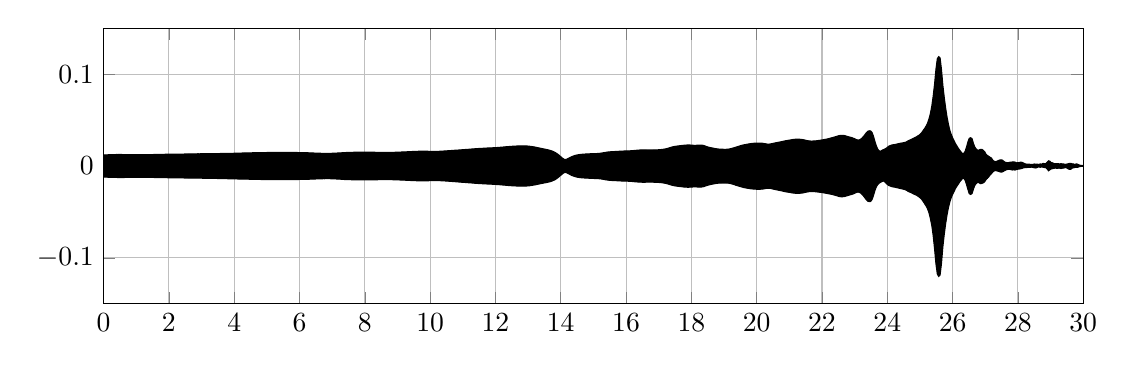
\begin{tikzpicture}

\begin{axis}[%
width=5.521in,
height=2in,
at={(0.758in,0.481in)},
xmin=0,
xmax=30,
xmajorgrids,
ymin=-0.15,
ymax=0.15,
ymajorgrids,
axis background/.style={fill=white}
]
\addplot[fill=black,draw=black,forget plot] plot table[row sep=crcr]{%
2.08333333333333e-05	0.0119891166687012\\
0.0425739952718676	0.0120701789855957\\
0.0851271572104019	0.0120600461959839\\
0.127680319148936	0.0121411085128784\\
0.17023348108747	0.0122112035751343\\
0.212786643026005	0.0122820138931274\\
0.255339804964539	0.0123153924942017\\
0.297892966903073	0.0123672485351563\\
0.340446128841608	0.0123822689056396\\
0.382999290780142	0.0124343633651733\\
0.425552452718676	0.012420654296875\\
0.46810561465721	0.0124455690383911\\
0.510658776595745	0.0124385356903076\\
0.553211938534279	0.0124293565750122\\
0.595765100472813	0.0124131441116333\\
0.638318262411347	0.0123996734619141\\
0.680871424349882	0.0123659372329712\\
0.723424586288416	0.0123772621154785\\
0.76597774822695	0.0123530626296997\\
0.808530910165485	0.0123927593231201\\
0.851084072104019	0.0123993158340454\\
0.893637234042553	0.0123468637466431\\
0.936190395981088	0.0123317241668701\\
0.978743557919622	0.0123351812362671\\
1.02129671985816	0.0123213529586792\\
1.06384988179669	0.012315034866333\\
1.10640304373522	0.0123295783996582\\
1.14895620567376	0.0123213529586792\\
1.19150936761229	0.012312650680542\\
1.23406252955083	0.0123451948165894\\
1.27661569148936	0.0123229026794434\\
1.3191688534279	0.0123435258865356\\
1.36172201536643	0.0123484134674072\\
1.40427517730496	0.0123796463012695\\
1.4468283392435	0.0123721361160278\\
1.48938150118203	0.0123879909515381\\
1.53193466312057	0.012427806854248\\
1.5744878250591	0.0124756097793579\\
1.61704098699764	0.012513279914856\\
1.65959414893617	0.0124995708465576\\
1.7021473108747	0.0125466585159302\\
1.74470047281324	0.012596607208252\\
1.78725363475177	0.0126116275787354\\
1.82980679669031	0.0126550197601318\\
1.87235995862884	0.012694239616394\\
1.91491312056738	0.0127073526382446\\
1.95746628250591	0.0127198696136475\\
2.00001944444444	0.0127586126327515\\
2.04257260638298	0.0127676725387573\\
2.08512576832151	0.012792706489563\\
2.12767893026005	0.0128316879272461\\
2.17023209219858	0.0128744840621948\\
2.21278525413712	0.0128858089447021\\
2.25533841607565	0.0128728151321411\\
2.29789157801418	0.0128904581069946\\
2.34044473995272	0.012937068939209\\
2.38299790189125	0.0129625797271729\\
2.42555106382979	0.0129508972167969\\
2.46810422576832	0.0129650831222534\\
2.51065738770686	0.0130186080932617\\
2.55321054964539	0.0130044221878052\\
2.59576371158392	0.0130490064620972\\
2.63831687352246	0.0130782127380371\\
2.68087003546099	0.0130912065505981\\
2.72342319739953	0.0131031274795532\\
2.76597635933806	0.0131406784057617\\
2.8085295212766	0.0131857395172119\\
2.85108268321513	0.0132355690002441\\
2.89363584515366	0.0132455825805664\\
2.9361890070922	0.0132309198379517\\
2.97874216903073	0.013269305229187\\
3.02129533096927	0.0133043527603149\\
3.0638484929078	0.013329029083252\\
3.10640165484634	0.0133227109909058\\
3.14895481678487	0.0133368968963623\\
3.1915079787234	0.0133442878723145\\
3.23406114066194	0.0133599042892456\\
3.27661430260047	0.0133839845657349\\
3.31916746453901	0.0133798122406006\\
3.36172062647754	0.0133849382400513\\
3.40427378841608	0.0134093761444092\\
3.44682695035461	0.013446569442749\\
3.48938011229314	0.0134661197662354\\
3.53193327423168	0.0134836435317993\\
3.57448643617021	0.013521671295166\\
3.61703959810875	0.0135370492935181\\
3.65959276004728	0.0135470628738403\\
3.70214592198582	0.0135759115219116\\
3.74469908392435	0.0136080980300903\\
3.78725224586288	0.0136371850967407\\
3.82980540780142	0.0136731863021851\\
3.87235856973995	0.0137186050415039\\
3.91491173167849	0.0137549638748169\\
3.95746489361702	0.0137441158294678\\
4.00001805555556	0.0138174295425415\\
4.04257121749409	0.013864278793335\\
4.08512437943262	0.0139147043228149\\
4.12767754137116	0.0139368772506714\\
4.17023070330969	0.0140061378479004\\
4.21278386524823	0.0140299797058105\\
4.25533702718676	0.0140790939331055\\
4.29789018912529	0.0141112804412842\\
4.34044335106383	0.0141588449478149\\
4.38299651300236	0.0141901969909668\\
4.4255496749409	0.0142172574996948\\
4.46810283687943	0.0142718553543091\\
4.51065599881797	0.0143095254898071\\
4.5532091607565	0.0143332481384277\\
4.59576232269503	0.0143661499023438\\
4.63831548463357	0.0144078731536865\\
4.6808686465721	0.0144317150115967\\
4.72342180851064	0.014464259147644\\
4.76597497044917	0.0144739151000977\\
4.80852813238771	0.0144917964935303\\
4.85108129432624	0.0145350694656372\\
4.89363445626477	0.0145490169525146\\
4.93618761820331	0.014581561088562\\
4.97874078014184	0.0145977735519409\\
5.02129394208038	0.0146069526672363\\
5.06384710401891	0.0146232843399048\\
5.10640026595745	0.0146393775939941\\
5.14895342789598	0.0146942138671875\\
5.19150658983452	0.0146994590759277\\
5.23405975177305	0.0147175788879395\\
5.27661291371158	0.0147092342376709\\
5.31916607565012	0.0147404670715332\\
5.36171923758865	0.0147354602813721\\
5.40427239952719	0.0147433280944824\\
5.44682556146572	0.0147520303726196\\
5.48937872340426	0.0147508382797241\\
5.53193188534279	0.0147504806518555\\
5.57448504728132	0.014761209487915\\
5.61703820921986	0.0147466659545898\\
5.65959137115839	0.0147426128387451\\
5.70214453309693	0.0147403478622437\\
5.74469769503546	0.0147124528884888\\
5.787250856974	0.0147058963775635\\
5.82980401891253	0.0147024393081665\\
5.87235718085106	0.0146327018737793\\
5.9149103427896	0.0146118402481079\\
5.95746350472813	0.0145947933197021\\
6.00001666666667	0.0145722627639771\\
6.0425698286052	0.0145455598831177\\
6.08512299054374	0.0144891738891602\\
6.12767615248227	0.0144437551498413\\
6.1702293144208	0.0144070386886597\\
6.21278247635934	0.014379620552063\\
6.25533563829787	0.0143579244613647\\
6.29788880023641	0.0142805576324463\\
6.34044196217494	0.0142168998718262\\
6.38299512411347	0.014191746711731\\
6.42554828605201	0.0140836238861084\\
6.46810144799054	0.0140348672866821\\
6.51065460992908	0.0139898061752319\\
6.55320777186761	0.0139384269714355\\
6.59576093380615	0.0138537883758545\\
6.63831409574468	0.0137983560562134\\
6.68086725768321	0.0137511491775513\\
6.72342041962175	0.0137094259262085\\
6.76597358156028	0.0136710405349731\\
6.80852674349882	0.0136563777923584\\
6.85107990543735	0.0136498212814331\\
6.89363306737589	0.0136363506317139\\
6.93618622931442	0.0136944055557251\\
6.97873939125296	0.0137603282928467\\
7.02129255319149	0.0138442516326904\\
7.06384571513002	0.0139046907424927\\
7.10639887706856	0.0139477252960205\\
7.14895203900709	0.014054536819458\\
7.19150520094563	0.0141353607177734\\
7.23405836288416	0.0142430067062378\\
7.27661152482269	0.0143053531646729\\
7.31916468676123	0.014385461807251\\
7.36171784869976	0.0145281553268433\\
7.4042710106383	0.0145792961120605\\
7.44682417257683	0.0146374702453613\\
7.48937733451537	0.014722466468811\\
7.5319304964539	0.0147558450698853\\
7.57448365839243	0.0148293972015381\\
7.61703682033097	0.0148519277572632\\
7.6595899822695	0.0148772001266479\\
7.70214314420804	0.0148836374282837\\
7.74469630614657	0.0149027109146118\\
7.78724946808511	0.0148898363113403\\
7.82980263002364	0.0149227380752563\\
7.87235579196217	0.0149306058883667\\
7.91490895390071	0.0149260759353638\\
7.95746211583924	0.0149365663528442\\
8.00001527777778	0.0149394273757935\\
8.04256843971631	0.0149445533752441\\
8.08512160165485	0.0149415731430054\\
8.12767476359338	0.0149654150009155\\
8.17022792553192	0.0149649381637573\\
8.21278108747045	0.014962911605835\\
8.25533424940898	0.0149157047271729\\
8.29788741134752	0.0148886442184448\\
8.34044057328605	0.0148481130599976\\
8.38299373522459	0.0147963762283325\\
8.42554689716312	0.0147671699523926\\
8.46810005910165	0.0147316455841064\\
8.51065322104019	0.0146907567977905\\
8.55320638297872	0.0146373510360718\\
8.59575954491726	0.0146878957748413\\
8.63831270685579	0.0146653652191162\\
8.68086586879433	0.0146582126617432\\
8.72341903073286	0.0146515369415283\\
8.76597219267139	0.0146892070770264\\
8.80852535460993	0.0147384405136108\\
8.85107851654846	0.0147976875305176\\
8.893631678487	0.0148004293441772\\
8.93618484042553	0.0149153470993042\\
8.97873800236407	0.0149699449539185\\
9.0212911643026	0.0150353908538818\\
9.06384432624114	0.0150772333145142\\
9.10639748817967	0.0151313543319702\\
9.1489506501182	0.0152260065078735\\
9.19150381205674	0.0153157711029053\\
9.23405697399527	0.015323281288147\\
9.27661013593381	0.0154021978378296\\
9.31916329787234	0.0154614448547363\\
9.36171645981088	0.0155340433120728\\
9.40426962174941	0.015607476234436\\
9.44682278368794	0.015711784362793\\
9.48937594562648	0.0157406330108643\\
9.53192910756501	0.0158414840698242\\
9.57448226950355	0.0159074068069458\\
9.61703543144208	0.0159391164779663\\
9.65958859338062	0.0160180330276489\\
9.70214175531915	0.0160245895385742\\
9.74469491725768	0.0160360336303711\\
9.78724807919622	0.01607346534729\\
9.82980124113475	0.0160551071166992\\
9.87235440307329	0.0160226821899414\\
9.91490756501182	0.0159975290298462\\
9.95746072695036	0.0159332752227783\\
10.0000138888889	0.0159041881561279\\
10.0425670508274	0.0158710479736328\\
10.085120212766	0.0158164501190186\\
10.1276733747045	0.0158092975616455\\
10.170226536643	0.0157977342605591\\
10.2127796985816	0.0158299207687378\\
10.2553328605201	0.0159136056900024\\
10.2978860224586	0.0159791707992554\\
10.3404391843972	0.016069769859314\\
10.3829923463357	0.0161577463150024\\
10.4255455082742	0.0162630081176758\\
10.4680986702128	0.0163758993148804\\
10.5106518321513	0.0164648294448853\\
10.5532049940898	0.0165594816207886\\
10.5957581560284	0.0166622400283813\\
10.6383113179669	0.016768217086792\\
10.6808644799054	0.0168865919113159\\
10.723417641844	0.0169931650161743\\
10.7659708037825	0.0171152353286743\\
10.808523965721	0.0171926021575928\\
10.8510771276596	0.017282247543335\\
10.8936302895981	0.0174212455749512\\
10.9361834515366	0.0175200700759888\\
10.9787366134752	0.0176385641098022\\
11.0212897754137	0.0177961587905884\\
11.0638429373522	0.0178617238998413\\
11.1063960992908	0.0179822444915771\\
11.1489492612293	0.0180516242980957\\
11.1915024231678	0.0181763172149658\\
11.2340555851064	0.0183032751083374\\
11.2766087470449	0.0184470415115356\\
11.3191619089835	0.0185744762420654\\
11.361715070922	0.0186715126037598\\
11.4042682328605	0.0187947750091553\\
11.4468213947991	0.0189191102981567\\
11.4893745567376	0.0189660787582397\\
11.5319277186761	0.0190688371658325\\
11.5744808806147	0.019160270690918\\
11.6170340425532	0.0192372798919678\\
11.6595872044917	0.0193090438842773\\
11.7021403664303	0.019400954246521\\
11.7446935283688	0.0195177793502808\\
11.7872466903073	0.0195590257644653\\
11.8297998522459	0.0196257829666138\\
11.8723530141844	0.0197001695632935\\
11.9149061761229	0.0197663307189941\\
11.9574593380615	0.0198649168014526\\
12.0000125	0.0199562311172485\\
12.0425656619385	0.0200393199920654\\
12.0851188238771	0.0201531648635864\\
12.1276719858156	0.0202683210372925\\
12.1702251477541	0.0203834772109985\\
12.2127783096927	0.0205181837081909\\
12.2553314716312	0.0206431150436401\\
12.2978846335697	0.020803689956665\\
12.3404377955083	0.0209430456161499\\
12.3829909574468	0.0210655927658081\\
12.4255441193853	0.0211613178253174\\
12.4680972813239	0.0213009119033813\\
12.5106504432624	0.0214111804962158\\
12.5532036052009	0.0215167999267578\\
12.5957567671395	0.0215667486190796\\
12.638309929078	0.0216765403747559\\
12.6808630910165	0.0217441320419312\\
12.7234162529551	0.0217874050140381\\
12.7659694148936	0.0218304395675659\\
12.8085225768322	0.0218579769134521\\
12.8510757387707	0.0218334197998047\\
12.8936289007092	0.0218534469604492\\
12.9361820626478	0.0217874050140381\\
12.9787352245863	0.0216927528381348\\
13.0212883865248	0.021544337272644\\
13.0638415484634	0.021371603012085\\
13.1063947104019	0.0211578607559204\\
13.1489478723404	0.0209262371063232\\
13.191501034279	0.0206685066223145\\
13.2340541962175	0.0203869342803955\\
13.276607358156	0.0200080871582031\\
13.3191605200946	0.019722580909729\\
13.3617136820331	0.0194058418273926\\
13.4042668439716	0.0190954208374023\\
13.4468200059102	0.0187587738037109\\
13.4893731678487	0.0184516906738281\\
13.5319263297872	0.0181584358215332\\
13.5744794917258	0.0178221464157104\\
13.6170326536643	0.0174729824066162\\
13.6595858156028	0.0171077251434326\\
13.7021389775414	0.016639232635498\\
13.7446921394799	0.0161151885986328\\
13.7872453014184	0.0154547691345215\\
13.829798463357	0.0146360397338867\\
13.8723516252955	0.0137324333190918\\
13.914904787234	0.0126259326934814\\
13.9574579491726	0.0113997459411621\\
14.0000111111111	0.0100481510162354\\
14.0425642730496	0.00874054431915283\\
14.0851174349882	0.00763881206512451\\
14.1276705969267	0.00698995590209961\\
14.1702237588652	0.00721240043640137\\
14.2127769208038	0.0078728199005127\\
14.2553300827423	0.00864839553833008\\
14.2978832446809	0.00943124294281006\\
14.3404364066194	0.010124683380127\\
14.3829895685579	0.0107450485229492\\
14.4255427304965	0.0112762451171875\\
14.468095892435	0.0117151737213135\\
14.5106490543735	0.0120129585266113\\
14.5532022163121	0.0122971534729004\\
14.5957553782506	0.0124787092208862\\
14.6383085401891	0.0126643180847168\\
14.6808617021277	0.0127860307693481\\
14.7234148640662	0.0129104852676392\\
14.7659680260047	0.013019323348999\\
14.8085211879433	0.0130923986434937\\
14.8510743498818	0.0131598711013794\\
14.8936275118203	0.0132442712783813\\
14.9361806737589	0.0132671594619751\\
14.9787338356974	0.0133401155471802\\
15.0212869976359	0.0133960247039795\\
15.0638401595745	0.0134508609771729\\
15.106393321513	0.0134987831115723\\
15.1489464834515	0.0135847330093384\\
15.1914996453901	0.0137389898300171\\
15.2340528073286	0.0139615535736084\\
15.2766059692671	0.0141968727111816\\
15.3191591312057	0.0144667625427246\\
15.3617122931442	0.0147184133529663\\
15.4042654550827	0.0149639844894409\\
15.4468186170213	0.0151892900466919\\
15.4893717789598	0.0153195858001709\\
15.5319249408983	0.0154467821121216\\
15.5744781028369	0.0155524015426636\\
15.6170312647754	0.0156270265579224\\
15.6595844267139	0.0157109498977661\\
15.7021375886525	0.0157914161682129\\
15.744690750591	0.0158919095993042\\
15.7872439125296	0.0159846544265747\\
15.8297970744681	0.0160763263702393\\
15.8723502364066	0.0161715745925903\\
15.9149033983452	0.0162194967269897\\
15.9574565602837	0.0162959098815918\\
16.0000097222222	0.0163196325302124\\
16.0425628841608	0.0163333415985107\\
16.0851160460993	0.0164139270782471\\
16.1276692080378	0.0164852142333984\\
16.1702223699764	0.016596794128418\\
16.2127755319149	0.0167173147201538\\
16.2553286938534	0.016867995262146\\
16.297881855792	0.0169942378997803\\
16.3404350177305	0.0171358585357666\\
16.382988179669	0.017247200012207\\
16.4255413416076	0.0173672437667847\\
16.4680945035461	0.0174224376678467\\
16.5106476654846	0.0174494981765747\\
16.5532008274232	0.0174441337585449\\
16.5957539893617	0.0174261331558228\\
16.6383071513002	0.0173689126968384\\
16.6808603132388	0.017351508140564\\
16.7234134751773	0.0173255205154419\\
16.7659666371158	0.0173234939575195\\
16.8085197990544	0.0173735618591309\\
16.8510729609929	0.0174065828323364\\
16.8936261229314	0.0174649953842163\\
16.93617928487	0.017520546913147\\
16.9787324468085	0.0175772905349731\\
17.021285608747	0.017709493637085\\
17.0638387706856	0.017842173576355\\
17.1063919326241	0.0179907083511353\\
17.1489450945626	0.0182030200958252\\
17.1914982565012	0.0184568166732788\\
17.2340514184397	0.0187783241271973\\
17.2766045803783	0.0191693305969238\\
17.3191577423168	0.0196816921234131\\
17.3617109042553	0.0201215744018555\\
17.4042640661939	0.0205991268157959\\
17.4468172281324	0.0209838151931763\\
17.4893703900709	0.0212384462356567\\
17.5319235520095	0.0214720964431763\\
17.574476713948	0.0217106342315674\\
17.6170298758865	0.0218876600265503\\
17.6595830378251	0.0220842361450195\\
17.7021361997636	0.0222510099411011\\
17.7446893617021	0.0224254131317139\\
17.7872425236407	0.0225731134414673\\
17.8297956855792	0.0227036476135254\\
17.8723488475177	0.0228030681610107\\
17.9149020094563	0.0228255987167358\\
17.9574551713948	0.0227867364883423\\
18.0000083333333	0.0226969718933105\\
18.0425614952719	0.0225468873977661\\
18.0851146572104	0.022442102432251\\
18.1276678191489	0.0224337577819824\\
18.1702209810875	0.0225523710250854\\
18.212774143026	0.0226941108703613\\
18.2553273049645	0.0227112770080566\\
18.2978804669031	0.0226702690124512\\
18.3404336288416	0.0225247144699097\\
18.3829867907801	0.022191047668457\\
18.4255399527187	0.0216506719589233\\
18.4680931146572	0.0210781097412109\\
18.5106462765957	0.0205855369567871\\
18.5531994385343	0.0202169418334961\\
18.5957526004728	0.0198911428451538\\
18.6383057624113	0.0195983648300171\\
18.6808589243499	0.0192761421203613\\
18.7234120862884	0.0189481973648071\\
18.765965248227	0.0187180042266846\\
18.8085184101655	0.0185004472732544\\
18.851071572104	0.0183453559875488\\
18.8936247340426	0.0182894468307495\\
18.9361778959811	0.018202543258667\\
18.9787310579196	0.0181392431259155\\
19.0212842198582	0.018133282661438\\
19.0638373817967	0.0181257724761963\\
19.1063905437352	0.0182130336761475\\
19.1489437056738	0.0184046030044556\\
19.1914968676123	0.0186821222305298\\
19.2340500295508	0.0190776586532593\\
19.2766031914894	0.0195093154907227\\
19.3191563534279	0.0199741125106812\\
19.3617095153664	0.020482063293457\\
19.404262677305	0.0209068059921265\\
19.4468158392435	0.0214110612869263\\
19.489369001182	0.0218472480773926\\
19.5319221631206	0.0223336219787598\\
19.5744753250591	0.0227125883102417\\
19.6170284869976	0.0230491161346436\\
19.6595816489362	0.0233137607574463\\
19.7021348108747	0.0236597061157227\\
19.7446879728132	0.0238858461380005\\
19.7872411347518	0.0241514444351196\\
19.8297942966903	0.0243535041809082\\
19.8723474586288	0.0245242118835449\\
19.9149006205674	0.0246922969818115\\
19.9574537825059	0.0247610807418823\\
20.0000069444444	0.0248315334320068\\
20.042560106383	0.0248575210571289\\
20.0851132683215	0.0248454809188843\\
20.12766643026	0.0248016119003296\\
20.1702195921986	0.0247161388397217\\
20.2127727541371	0.0244866609573364\\
20.2553259160756	0.0242441892623901\\
20.2978790780142	0.0239566564559937\\
20.3404322399527	0.0237118005752563\\
20.3829854018913	0.0237652063369751\\
20.4255385638298	0.0240160226821899\\
20.4680917257683	0.0243251323699951\\
20.5106448877069	0.0246405601501465\\
20.5531980496454	0.0249805450439453\\
20.5957512115839	0.0253318548202515\\
20.6383043735225	0.025571346282959\\
20.680857535461	0.0258880853652954\\
20.7234106973995	0.0261416435241699\\
20.7659638593381	0.0264977216720581\\
20.8085170212766	0.0268567800521851\\
20.8510701832151	0.0271531343460083\\
20.8936233451537	0.0274865627288818\\
20.9361765070922	0.027751088142395\\
20.9787296690307	0.0279955863952637\\
21.0212828309693	0.0282137393951416\\
21.0638359929078	0.0284777879714966\\
21.1063891548463	0.0287666320800781\\
21.1489423167849	0.0289372205734253\\
21.1914954787234	0.0290979146957397\\
21.2340486406619	0.0291520357131958\\
21.2766018026005	0.0291374921798706\\
21.319154964539	0.0290536880493164\\
21.3617081264775	0.0289229154586792\\
21.4042612884161	0.0287134647369385\\
21.4468144503546	0.0284314155578613\\
21.4893676122931	0.0280815362930298\\
21.5319207742317	0.0277200937271118\\
21.5744739361702	0.027424693107605\\
21.6170270981087	0.0271998643875122\\
21.6595802600473	0.0271004438400269\\
21.7021334219858	0.0271096229553223\\
21.7446865839243	0.027174711227417\\
21.7872397458629	0.0272704362869263\\
21.8297929078014	0.0274029970169067\\
21.87234606974	0.0276217460632324\\
21.9148992316785	0.0278003215789795\\
21.957452393617	0.0280568599700928\\
22.0000055555556	0.028328537940979\\
22.0425587174941	0.0285825729370117\\
22.0851118794326	0.0288678407669067\\
22.1276650413712	0.0291299819946289\\
22.1702182033097	0.029487133026123\\
22.2127713652482	0.029843807220459\\
22.2553245271868	0.0302610397338867\\
22.2978776891253	0.0306540727615356\\
22.3404308510638	0.0310933589935303\\
22.3829840130024	0.0315306186676025\\
22.4255371749409	0.0319411754608154\\
22.4680903368794	0.0324456691741943\\
22.510643498818	0.0329251289367676\\
22.5531966607565	0.0331741571426392\\
22.595749822695	0.0333001613616943\\
22.6383029846336	0.0332827568054199\\
22.6808561465721	0.0331307649612427\\
22.7234093085106	0.0327298641204834\\
22.7659624704492	0.032257080078125\\
22.8085156323877	0.0318152904510498\\
22.8510687943262	0.0313825607299805\\
22.8936219562648	0.0310475826263428\\
22.9361751182033	0.0305105447769165\\
22.9787282801418	0.0299614667892456\\
23.0212814420804	0.0292130708694458\\
23.0638346040189	0.0285649299621582\\
23.1063877659574	0.0281169414520264\\
23.148940927896	0.0285003185272217\\
23.1914940898345	0.0293340682983398\\
23.234047251773	0.0306720733642578\\
23.2766004137116	0.0323584079742432\\
23.3191535756501	0.0342948436737061\\
23.3617067375887	0.0363030433654785\\
23.4042598995272	0.0377959012985229\\
23.4468130614657	0.0382936000823975\\
23.4893662234043	0.0381671190261841\\
23.5319193853428	0.0364677906036377\\
23.5744725472813	0.0325307846069336\\
23.6170257092199	0.0271339416503906\\
23.6595788711584	0.0222088098526001\\
23.7021320330969	0.0186933279037476\\
23.7446851950355	0.0165317058563232\\
23.787238356974	0.0160146951675415\\
23.8297915189125	0.0168312788009644\\
23.8723446808511	0.0176469087600708\\
23.9148978427896	0.018263578414917\\
23.9574510047281	0.018985390663147\\
24.0000041666667	0.0202053785324097\\
24.0425573286052	0.0214619636535645\\
24.0851104905437	0.022052526473999\\
24.1276636524823	0.0227371454238892\\
24.1702168144208	0.0230492353439331\\
24.2127699763593	0.0232532024383545\\
24.2553231382979	0.0234876871109009\\
24.2978763002364	0.0238732099533081\\
24.3404294621749	0.0242279767990112\\
24.3829826241135	0.0246217250823975\\
24.425535786052	0.0249172449111938\\
24.4680889479905	0.0250427722930908\\
24.5106421099291	0.0254533290863037\\
24.5531952718676	0.0256302356719971\\
24.5957484338061	0.0264087915420532\\
24.6383015957447	0.0274142026901245\\
24.6808547576832	0.028038501739502\\
24.7234079196217	0.0287498235702515\\
24.7659610815603	0.029454231262207\\
24.8085142434988	0.0302711725234985\\
24.8510674054374	0.0310555696487427\\
24.8936205673759	0.0316926240921021\\
24.9361737293144	0.0327839851379395\\
24.978726891253	0.033631443977356\\
25.0212800531915	0.0349727869033813\\
25.06383321513	0.0368019342422485\\
25.1063863770686	0.0389444828033447\\
25.1489395390071	0.041167140007019\\
25.1914927009456	0.0434926748275757\\
25.2340458628842	0.0467634201049805\\
25.2765990248227	0.0511188507080078\\
25.3191521867612	0.057016134262085\\
25.3617053486998	0.0649584531784058\\
25.4042585106383	0.0758386850357056\\
25.4468116725768	0.0889134407043457\\
25.4893648345154	0.105216860771179\\
25.5319179964539	0.116796731948853\\
25.5744711583924	0.119030594825745\\
25.617024320331	0.11763870716095\\
25.6595774822695	0.104707360267639\\
25.702130644208	0.0874937772750854\\
25.7446838061466	0.0744110345840454\\
25.7872369680851	0.06288743019104\\
25.8297901300236	0.0530766248703003\\
25.8723432919622	0.0452847480773926\\
25.9148964539007	0.0387722253799438\\
25.9574496158392	0.0343474149703979\\
26.0000027777778	0.030636191368103\\
26.0425559397163	0.0276141166687012\\
26.0851091016548	0.0244072675704956\\
26.1276622635934	0.0219786167144775\\
26.1702154255319	0.0195002555847168\\
26.2127685874705	0.017353892326355\\
26.255321749409	0.0152941942214966\\
26.2978749113475	0.0136313438415527\\
26.3404280732861	0.0135471820831299\\
26.3829812352246	0.0158743858337402\\
26.4255343971631	0.0204313993453979\\
26.4680875591017	0.0261033773422241\\
26.5106407210402	0.0301426649093628\\
26.5531938829787	0.0307470560073853\\
26.5957470449173	0.0297296047210693\\
26.6383002068558	0.0243973731994629\\
26.6808533687943	0.0204536914825439\\
26.7234065307329	0.0183995962142944\\
26.7659596926714	0.0170893669128418\\
26.8085128546099	0.0173263549804688\\
26.8510660165485	0.01812744140625\\
26.893619178487	0.0181320905685425\\
26.9361723404255	0.0170766115188599\\
26.9787255023641	0.0156316757202148\\
27.0212786643026	0.0127568244934082\\
27.0638318262411	0.0114500522613525\\
27.1063849881797	0.0104755163192749\\
27.1489381501182	0.00944781303405762\\
27.1914913120567	0.00852572917938232\\
27.2340444739953	0.00608611106872559\\
27.2765976359338	0.00501561164855957\\
27.3191507978723	0.00464582443237305\\
27.3617039598109	0.0052187442779541\\
27.4042571217494	0.00589883327484131\\
27.4468102836879	0.00653588771820068\\
27.4893634456265	0.00666952133178711\\
27.531916607565	0.00618875026702881\\
27.5744697695035	0.00481438636779785\\
27.6170229314421	0.00392997264862061\\
27.6595760933806	0.00364542007446289\\
27.7021292553192	0.00357687473297119\\
27.7446824172577	0.0039665699005127\\
27.7872355791962	0.00409770011901855\\
27.8297887411348	0.00434184074401855\\
27.8723419030733	0.00437593460083008\\
27.9148950650118	0.00416827201843262\\
27.9574482269504	0.00337409973144531\\
28.0000013888889	0.00351810455322266\\
28.0425545508274	0.00388240814208984\\
28.085107712766	0.00404250621795654\\
28.1276608747045	0.00395500659942627\\
28.170214036643	0.0031973123550415\\
28.2127671985816	0.00237417221069336\\
28.2553203605201	0.00200951099395752\\
28.2978735224586	0.00202393531799316\\
28.3404266843972	0.00191807746887207\\
28.3829798463357	0.00173366069793701\\
28.4255330082742	0.00155413150787354\\
28.4680861702128	0.00181210041046143\\
28.5106393321513	0.00211071968078613\\
28.5531924940898	0.00176608562469482\\
28.5957456560284	0.00202560424804688\\
28.6382988179669	0.00156760215759277\\
28.6808519799054	0.00219047069549561\\
28.723405141844	0.00191926956176758\\
28.7659583037825	0.00270414352416992\\
28.808511465721	0.00257468223571777\\
28.8510646276596	0.00250673294067383\\
28.8936177895981	0.00388991832733154\\
28.9361709515366	0.00561344623565674\\
28.9787241134752	0.00521004199981689\\
29.0212772754137	0.00365424156188965\\
29.0638304373522	0.0033804178237915\\
29.1063835992908	0.00262355804443359\\
29.1489367612293	0.00234818458557129\\
29.1914899231679	0.0025477409362793\\
29.2340430851064	0.00256478786468506\\
29.2765962470449	0.00208735466003418\\
29.3191494089835	0.00250005722045898\\
29.361702570922	0.00219547748565674\\
29.4042557328605	0.00211131572723389\\
29.4468088947991	0.00169658660888672\\
29.4893620567376	0.00201320648193359\\
29.5319152186761	0.00230777263641357\\
29.5744683806147	0.00270867347717285\\
29.6170215425532	0.0027766227722168\\
29.6595747044917	0.00231611728668213\\
29.7021278664303	0.00214874744415283\\
29.7446810283688	0.00160884857177734\\
29.7872341903073	0.00224554538726807\\
29.8297873522459	0.00190925598144531\\
29.8723405141844	0.00109612941741943\\
29.9148936761229	0.000704288482666016\\
29.9574468380615	0.00048518180847168\\
30	0.000414729118347168\\
}
\closedcycle;
\addplot[fill=black,draw=black,forget plot] plot table[row sep=crcr]{%
2.08333333333333e-05	-0.012113094329834\\
0.0425739952718676	-0.0121138095855713\\
0.0851271572104019	-0.0121619701385498\\
0.127680319148936	-0.0122429132461548\\
0.17023348108747	-0.0122907161712646\\
0.212786643026005	-0.0123883485794067\\
0.255339804964539	-0.0124168395996094\\
0.297892966903073	-0.0124434232711792\\
0.340446128841608	-0.01246178150177\\
0.382999290780142	-0.0125032663345337\\
0.425552452718676	-0.0125099420547485\\
0.46810561465721	-0.0125166177749634\\
0.510658776595745	-0.0125166177749634\\
0.553211938534279	-0.0125176906585693\\
0.595765100472813	-0.0125076770782471\\
0.638318262411347	-0.0125123262405396\\
0.680871424349882	-0.0124843120574951\\
0.723424586288416	-0.0124874114990234\\
0.76597774822695	-0.0124468803405762\\
0.808530910165485	-0.0124509334564209\\
0.851084072104019	-0.0124367475509644\\
0.893637234042553	-0.0124189853668213\\
0.936190395981088	-0.012392520904541\\
0.978743557919622	-0.0124033689498901\\
1.02129671985816	-0.0123730897903442\\
1.06384988179669	-0.0124198198318481\\
1.10640304373522	-0.0123876333236694\\
1.14895620567376	-0.0124117136001587\\
1.19150936761229	-0.0123980045318604\\
1.23406252955083	-0.0124258995056152\\
1.27661569148936	-0.012415885925293\\
1.3191688534279	-0.0124626159667969\\
1.36172201536643	-0.012446403503418\\
1.40427517730496	-0.0124740600585938\\
1.4468283392435	-0.0124877691268921\\
1.48938150118203	-0.0125036239624023\\
1.53193466312057	-0.0125057697296143\\
1.5744878250591	-0.0125240087509155\\
1.61704098699764	-0.0125665664672852\\
1.65959414893617	-0.012586236000061\\
1.7021473108747	-0.0126203298568726\\
1.74470047281324	-0.0126328468322754\\
1.78725363475177	-0.0126634836196899\\
1.82980679669031	-0.0127276182174683\\
1.87235995862884	-0.0127447843551636\\
1.91491312056738	-0.0127626657485962\\
1.95746628250591	-0.0127805471420288\\
2.00001944444444	-0.0128178596496582\\
2.04257260638298	-0.0128737688064575\\
2.08512576832151	-0.0128716230392456\\
2.12767893026005	-0.0129257440567017\\
2.17023209219858	-0.0129240751266479\\
2.21278525413712	-0.0129307508468628\\
2.25533841607565	-0.0129609107971191\\
2.29789157801418	-0.0129433870315552\\
2.34044473995272	-0.0129650831222534\\
2.38299790189125	-0.012988805770874\\
2.42555106382979	-0.013023853302002\\
2.46810422576832	-0.0130585432052612\\
2.51065738770686	-0.0130890607833862\\
2.55321054964539	-0.0130822658538818\\
2.59576371158392	-0.0131436586380005\\
2.63831687352246	-0.0131477117538452\\
2.68087003546099	-0.0131758451461792\\
2.72342319739953	-0.0131961107254028\\
2.76597635933806	-0.0131841897964478\\
2.8085295212766	-0.0132342576980591\\
2.85108268321513	-0.0132158994674683\\
2.89363584515366	-0.0132571458816528\\
2.9361890070922	-0.0132758617401123\\
2.97874216903073	-0.0133143663406372\\
3.02129533096927	-0.0133262872695923\\
3.0638484929078	-0.0133285522460938\\
3.10640165484634	-0.0133302211761475\\
3.14895481678487	-0.0133769512176514\\
3.1915079787234	-0.0133914947509766\\
3.23406114066194	-0.013434886932373\\
3.27661430260047	-0.0134336948394775\\
3.31916746453901	-0.0134991407394409\\
3.36172062647754	-0.0134928226470947\\
3.40427378841608	-0.0135328769683838\\
3.44682695035461	-0.0135462284088135\\
3.48938011229314	-0.0136126279830933\\
3.53193327423168	-0.0136435031890869\\
3.57448643617021	-0.0136560201644897\\
3.61703959810875	-0.0137197971343994\\
3.65959276004728	-0.0137335062026978\\
3.70214592198582	-0.0137761831283569\\
3.74469908392435	-0.013823390007019\\
3.78725224586288	-0.0138667821884155\\
3.82980540780142	-0.0138909816741943\\
3.87235856973995	-0.0139669179916382\\
3.91491173167849	-0.013978123664856\\
3.95746489361702	-0.0140331983566284\\
4.00001805555556	-0.0140602588653564\\
4.04257121749409	-0.0141162872314453\\
4.08512437943262	-0.0141328573226929\\
4.12767754137116	-0.0141587257385254\\
4.17023070330969	-0.0142300128936768\\
4.21278386524823	-0.0142171382904053\\
4.25533702718676	-0.0142806768417358\\
4.29789018912529	-0.0142964124679565\\
4.34044335106383	-0.0143094062805176\\
4.38299651300236	-0.014351487159729\\
4.4255496749409	-0.0144045352935791\\
4.46810283687943	-0.0144202709197998\\
4.51065599881797	-0.0144541263580322\\
4.5532091607565	-0.0145096778869629\\
4.59576232269503	-0.0145117044448853\\
4.63831548463357	-0.0145535469055176\\
4.6808686465721	-0.0145788192749023\\
4.72342180851064	-0.0146294832229614\\
4.76597497044917	-0.0146406888961792\\
4.80852813238771	-0.0146827697753906\\
4.85108129432624	-0.0147362947463989\\
4.89363445626477	-0.0147140026092529\\
4.93618761820331	-0.014751672744751\\
4.97874078014184	-0.0147874355316162\\
5.02129394208038	-0.0148072242736816\\
5.06384710401891	-0.0147817134857178\\
5.10640026595745	-0.0148316621780396\\
5.14895342789598	-0.0148299932479858\\
5.19150658983452	-0.0148706436157227\\
5.23405975177305	-0.0148839950561523\\
5.27661291371158	-0.0149160623550415\\
5.31916607565012	-0.0149294137954712\\
5.36171923758865	-0.0149381160736084\\
5.40427239952719	-0.0149247646331787\\
5.44682556146572	-0.0149132013320923\\
5.48937872340426	-0.0149377584457397\\
5.53193188534279	-0.014884352684021\\
5.57448504728132	-0.0148860216140747\\
5.61703820921986	-0.0148693323135376\\
5.65959137115839	-0.0148825645446777\\
5.70214453309693	-0.0148489475250244\\
5.74469769503546	-0.0148134231567383\\
5.787250856974	-0.0148054361343384\\
5.82980401891253	-0.0147805213928223\\
5.87235718085106	-0.0147774219512939\\
5.9149103427896	-0.014757513999939\\
5.95746350472813	-0.014722466468811\\
6.00001666666667	-0.0146836042404175\\
6.0425698286052	-0.0146520137786865\\
6.08512299054374	-0.0146064758300781\\
6.12767615248227	-0.0145918130874634\\
6.1702293144208	-0.0145655870437622\\
6.21278247635934	-0.0145376920700073\\
6.25533563829787	-0.0144726037979126\\
6.29788880023641	-0.0144317150115967\\
6.34044196217494	-0.0143640041351318\\
6.38299512411347	-0.0143401622772217\\
6.42554828605201	-0.0142568349838257\\
6.46810144799054	-0.0141904354095459\\
6.51065460992908	-0.014129638671875\\
6.55320777186761	-0.0140664577484131\\
6.59576093380615	-0.0139951705932617\\
6.63831409574468	-0.0139943361282349\\
6.68086725768321	-0.013921856880188\\
6.72342041962175	-0.0138674974441528\\
6.76597358156028	-0.0138700008392334\\
6.80852674349882	-0.0138266086578369\\
6.85107990543735	-0.0138033628463745\\
6.89363306737589	-0.0138267278671265\\
6.93618622931442	-0.0138603448867798\\
6.97873939125296	-0.0139093399047852\\
7.02129255319149	-0.0139569044113159\\
7.06384571513002	-0.0140078067779541\\
7.10639887706856	-0.0141046047210693\\
7.14895203900709	-0.0142216682434082\\
7.19150520094563	-0.0143018960952759\\
7.23405836288416	-0.014325737953186\\
7.27661152482269	-0.0144776105880737\\
7.31916468676123	-0.014553427696228\\
7.36171784869976	-0.0146636962890625\\
7.4042710106383	-0.0147805213928223\\
7.44682417257683	-0.0147774219512939\\
7.48937733451537	-0.0148789882659912\\
7.5319304964539	-0.014926552772522\\
7.57448365839243	-0.0149526596069336\\
7.61703682033097	-0.0149977207183838\\
7.6595899822695	-0.0150274038314819\\
7.70214314420804	-0.0150216817855835\\
7.74469630614657	-0.0150569677352905\\
7.78724946808511	-0.0150774717330933\\
7.82980263002364	-0.0150794982910156\\
7.87235579196217	-0.0150913000106812\\
7.91490895390071	-0.0150800943374634\\
7.95746211583924	-0.0151046514511108\\
8.00001527777778	-0.0151209831237793\\
8.04256843971631	-0.0151158571243286\\
8.08512160165485	-0.0151230096817017\\
8.12767476359338	-0.0151163339614868\\
8.17022792553192	-0.0151170492172241\\
8.21278108747045	-0.015113353729248\\
8.25533424940898	-0.0150854587554932\\
8.29788741134752	-0.0150784254074097\\
8.34044057328605	-0.014992356300354\\
8.38299373522459	-0.0149698257446289\\
8.42554689716312	-0.0149426460266113\\
8.46810005910165	-0.014917254447937\\
8.51065322104019	-0.0148546695709229\\
8.55320638297872	-0.014845609664917\\
8.59575954491726	-0.0148199796676636\\
8.63831270685579	-0.014836311340332\\
8.68086586879433	-0.0148338079452515\\
8.72341903073286	-0.01482093334198\\
8.76597219267139	-0.0148725509643555\\
8.80852535460993	-0.0149130821228027\\
8.85107851654846	-0.0149532556533813\\
8.893631678487	-0.0150277614593506\\
8.93618484042553	-0.0150550603866577\\
8.97873800236407	-0.0151125192642212\\
9.0212911643026	-0.0151705741882324\\
9.06384432624114	-0.0152268409729004\\
9.10639748817967	-0.0152989625930786\\
9.1489506501182	-0.0153621435165405\\
9.19150381205674	-0.0154212713241577\\
9.23405697399527	-0.0154908895492554\\
9.27661013593381	-0.0155407190322876\\
9.31916329787234	-0.0156335830688477\\
9.36171645981088	-0.0156954526901245\\
9.40426962174941	-0.0157989263534546\\
9.44682278368794	-0.0158728361129761\\
9.48937594562648	-0.0159257650375366\\
9.53192910756501	-0.0159800052642822\\
9.57448226950355	-0.0160501003265381\\
9.61703543144208	-0.0160759687423706\\
9.65958859338062	-0.0161364078521729\\
9.70214175531915	-0.0161623954772949\\
9.74469491725768	-0.0161715745925903\\
9.78724807919622	-0.0161818265914917\\
9.82980124113475	-0.0161776542663574\\
9.87235440307329	-0.0161452293395996\\
9.91490756501182	-0.0161435604095459\\
9.95746072695036	-0.0160480737686157\\
10.0000138888889	-0.0160074234008789\\
10.0425670508274	-0.0159573554992676\\
10.085120212766	-0.0158952474594116\\
10.1276733747045	-0.0158969163894653\\
10.170226536643	-0.0158489942550659\\
10.2127796985816	-0.0158857107162476\\
10.2553328605201	-0.0159428119659424\\
10.2978860224586	-0.0159850120544434\\
10.3404391843972	-0.0160963535308838\\
10.3829923463357	-0.0161405801773071\\
10.4255455082742	-0.0162266492843628\\
10.4680986702128	-0.0163537263870239\\
10.5106518321513	-0.016463041305542\\
10.5532049940898	-0.0165412425994873\\
10.5957581560284	-0.0166654586791992\\
10.6383113179669	-0.0167874097824097\\
10.6808644799054	-0.0168699026107788\\
10.723417641844	-0.0170114040374756\\
10.7659708037825	-0.0171157121658325\\
10.808523965721	-0.0172432661056519\\
10.8510771276596	-0.0173588991165161\\
10.8936302895981	-0.0174890756607056\\
10.9361834515366	-0.0176196098327637\\
10.9787366134752	-0.0177257061004639\\
11.0212897754137	-0.0178505182266235\\
11.0638429373522	-0.0179296731948853\\
11.1063960992908	-0.0180578231811523\\
11.1489492612293	-0.0181858539581299\\
11.1915024231678	-0.0183118581771851\\
11.2340555851064	-0.0184283256530762\\
11.2766087470449	-0.0185163021087646\\
11.3191619089835	-0.0186553001403809\\
11.361715070922	-0.018781304359436\\
11.4042682328605	-0.0188863277435303\\
11.4468213947991	-0.0190004110336304\\
11.4893745567376	-0.0191012620925903\\
11.5319277186761	-0.0192080736160278\\
11.5744808806147	-0.0192803144454956\\
11.6170340425532	-0.0193767547607422\\
11.6595872044917	-0.019465446472168\\
11.7021403664303	-0.0195423364639282\\
11.7446935283688	-0.0196044445037842\\
11.7872466903073	-0.0196491479873657\\
11.8297998522459	-0.0197625160217285\\
11.8723530141844	-0.019813060760498\\
11.9149061761229	-0.0199345350265503\\
11.9574593380615	-0.0199878215789795\\
12.0000125	-0.0200809240341187\\
12.0425656619385	-0.020203709602356\\
12.0851188238771	-0.0202950239181519\\
12.1276719858156	-0.0203992128372192\\
12.1702251477541	-0.0205478668212891\\
12.2127783096927	-0.0206730365753174\\
12.2553314716312	-0.0208123922348022\\
12.2978846335697	-0.0209157466888428\\
12.3404377955083	-0.0210793018341064\\
12.3829909574468	-0.0212075710296631\\
12.4255441193853	-0.0213204622268677\\
12.4680972813239	-0.0214297771453857\\
12.5106504432624	-0.0215437412261963\\
12.5532036052009	-0.0216523408889771\\
12.5957567671395	-0.0217057466506958\\
12.638309929078	-0.0217827558517456\\
12.6808630910165	-0.0218445062637329\\
12.7234162529551	-0.0219008922576904\\
12.7659694148936	-0.0219255685806274\\
12.8085225768322	-0.0219546556472778\\
12.8510757387707	-0.0219559669494629\\
12.8936289007092	-0.0219188928604126\\
12.9361820626478	-0.0218608379364014\\
12.9787352245863	-0.0217357873916626\\
13.0212883865248	-0.0215924978256226\\
13.0638415484634	-0.0214599370956421\\
13.1063947104019	-0.0211890935897827\\
13.1489478723404	-0.0209450721740723\\
13.191501034279	-0.0206962823867798\\
13.2340541962175	-0.0204030275344849\\
13.276607358156	-0.0200580358505249\\
13.3191605200946	-0.0197618007659912\\
13.3617136820331	-0.0194422006607056\\
13.4042668439716	-0.0191107988357544\\
13.4468200059102	-0.0188400745391846\\
13.4893731678487	-0.0184996128082275\\
13.5319263297872	-0.0182305574417114\\
13.5744794917258	-0.0179266929626465\\
13.6170326536643	-0.017613410949707\\
13.6595858156028	-0.0172340869903564\\
13.7021389775414	-0.0167717933654785\\
13.7446921394799	-0.0162343978881836\\
13.7872453014184	-0.0155785083770752\\
13.829798463357	-0.0147982835769653\\
13.8723516252955	-0.0138078927993774\\
13.914904787234	-0.0126904249191284\\
13.9574579491726	-0.0114437341690063\\
14.0000111111111	-0.0101087093353271\\
14.0425642730496	-0.00886237621307373\\
14.0851174349882	-0.00769996643066406\\
14.1276705969267	-0.00697076320648193\\
14.1702237588652	-0.00723934173583984\\
14.2127769208038	-0.0079423189163208\\
14.2553300827423	-0.00873672962188721\\
14.2978832446809	-0.00956249237060547\\
14.3404364066194	-0.010346531867981\\
14.3829895685579	-0.0109330415725708\\
14.4255427304965	-0.0114353895187378\\
14.468095892435	-0.0118498802185059\\
14.5106490543735	-0.0122239589691162\\
14.5532022163121	-0.0124701261520386\\
14.5957553782506	-0.0126818418502808\\
14.6383085401891	-0.0128611326217651\\
14.6808617021277	-0.0129830837249756\\
14.7234148640662	-0.013073205947876\\
14.7659680260047	-0.0131728649139404\\
14.8085211879433	-0.0132454633712769\\
14.8510743498818	-0.0133155584335327\\
14.8936275118203	-0.0134053230285645\\
14.9361806737589	-0.0134707689285278\\
14.9787338356974	-0.013554573059082\\
15.0212869976359	-0.0136101245880127\\
15.0638401595745	-0.0136501789093018\\
15.106393321513	-0.0137456655502319\\
15.1489464834515	-0.0138136148452759\\
15.1914996453901	-0.0139260292053223\\
15.2340528073286	-0.0141358375549316\\
15.2766059692671	-0.0143586397171021\\
15.3191591312057	-0.0146870613098145\\
15.3617122931442	-0.0149590969085693\\
15.4042654550827	-0.0151717662811279\\
15.4468186170213	-0.0154045820236206\\
15.4893717789598	-0.0155810117721558\\
15.5319249408983	-0.015711784362793\\
15.5744781028369	-0.0158271789550781\\
15.6170312647754	-0.0158728361129761\\
15.6595844267139	-0.0159279108047485\\
15.7021375886525	-0.016033411026001\\
15.744690750591	-0.016116738319397\\
15.7872439125296	-0.0162032842636108\\
15.8297970744681	-0.016295313835144\\
15.8723502364066	-0.0163846015930176\\
15.9149033983452	-0.0164285898208618\\
15.9574565602837	-0.016472339630127\\
16.0000097222222	-0.0165252685546875\\
16.0425628841608	-0.0165561437606812\\
16.0851160460993	-0.0166240930557251\\
16.1276692080378	-0.0167051553726196\\
16.1702223699764	-0.0168216228485107\\
16.2127755319149	-0.0169605016708374\\
16.2553286938534	-0.0171339511871338\\
16.297881855792	-0.017236590385437\\
16.3404350177305	-0.0173897743225098\\
16.382988179669	-0.0175108909606934\\
16.4255413416076	-0.0175718069076538\\
16.4680945035461	-0.0176539421081543\\
16.5106476654846	-0.0177140235900879\\
16.5532008274232	-0.0177189111709595\\
16.5957539893617	-0.0176827907562256\\
16.6383071513002	-0.0176247358322144\\
16.6808603132388	-0.0176045894622803\\
16.7234134751773	-0.0175678730010986\\
16.7659666371158	-0.0176085233688354\\
16.8085197990544	-0.0176388025283813\\
16.8510729609929	-0.0176856517791748\\
16.8936261229314	-0.0177114009857178\\
16.93617928487	-0.0177881717681885\\
16.9787324468085	-0.0179146528244019\\
17.021285608747	-0.0179815292358398\\
17.0638387706856	-0.0181503295898438\\
17.1063919326241	-0.0182839632034302\\
17.1489450945626	-0.0185275077819824\\
17.1914982565012	-0.0188034772872925\\
17.2340514184397	-0.019094705581665\\
17.2766045803783	-0.0195196866989136\\
17.3191577423168	-0.0200101137161255\\
17.3617109042553	-0.0204836130142212\\
17.4042640661939	-0.0209158658981323\\
17.4468172281324	-0.0212987661361694\\
17.4893703900709	-0.0215929746627808\\
17.5319235520095	-0.021852970123291\\
17.574476713948	-0.0220389366149902\\
17.6170298758865	-0.0222564935684204\\
17.6595830378251	-0.0223824977874756\\
17.7021361997636	-0.0225727558135986\\
17.7446893617021	-0.0228184461593628\\
17.7872425236407	-0.022945761680603\\
17.8297956855792	-0.0230010747909546\\
17.8723488475177	-0.0231268405914307\\
17.9149020094563	-0.023140549659729\\
17.9574551713948	-0.0230916738510132\\
18.0000083333333	-0.0230250358581543\\
18.0425614952719	-0.0228646993637085\\
18.0851146572104	-0.0227128267288208\\
18.1276678191489	-0.0227124691009521\\
18.1702209810875	-0.02284836769104\\
18.212774143026	-0.0229490995407104\\
18.2553273049645	-0.0229932069778442\\
18.2978804669031	-0.0229518413543701\\
18.3404336288416	-0.0227921009063721\\
18.3829867907801	-0.0224471092224121\\
18.4255399527187	-0.0218509435653687\\
18.4680931146572	-0.0213072299957275\\
18.5106462765957	-0.0208621025085449\\
18.5531994385343	-0.020465612411499\\
18.5957526004728	-0.0201561450958252\\
18.6383057624113	-0.0198447704315186\\
18.6808589243499	-0.019536018371582\\
18.7234120862884	-0.0192290544509888\\
18.765965248227	-0.019008994102478\\
18.8085184101655	-0.0188168287277222\\
18.851071572104	-0.0186343193054199\\
18.8936247340426	-0.0186009407043457\\
18.9361778959811	-0.0185483694076538\\
18.9787310579196	-0.0185364484786987\\
19.0212842198582	-0.018534779548645\\
19.0638373817967	-0.0185306072235107\\
19.1063905437352	-0.0186336040496826\\
19.1489437056738	-0.0188100337982178\\
19.1914968676123	-0.0191055536270142\\
19.2340500295508	-0.0194660425186157\\
19.2766031914894	-0.0199325084686279\\
19.3191563534279	-0.0204150676727295\\
19.3617095153664	-0.0209709405899048\\
19.404262677305	-0.0214064121246338\\
19.4468158392435	-0.0218608379364014\\
19.489369001182	-0.0222972631454468\\
19.5319221631206	-0.0227186679840088\\
19.5744753250591	-0.0231914520263672\\
19.6170284869976	-0.0235624313354492\\
19.6595816489362	-0.0238556861877441\\
19.7021348108747	-0.024156928062439\\
19.7446879728132	-0.0243837833404541\\
19.7872411347518	-0.0246430635452271\\
19.8297942966903	-0.0248475074768066\\
19.8723474586288	-0.0250301361083984\\
19.9149006205674	-0.0251462459564209\\
19.9574537825059	-0.0252714157104492\\
20.0000069444444	-0.0253260135650635\\
20.042560106383	-0.0253632068634033\\
20.0851132683215	-0.0253657102584839\\
20.12766643026	-0.0252941846847534\\
20.1702195921986	-0.0252175331115723\\
20.2127727541371	-0.0249605178833008\\
20.2553259160756	-0.0246913433074951\\
20.2978790780142	-0.0244394540786743\\
20.3404322399527	-0.0242527723312378\\
20.3829854018913	-0.0242507457733154\\
20.4255385638298	-0.0244895219802856\\
20.4680917257683	-0.024840235710144\\
20.5106448877069	-0.0251890420913696\\
20.5531980496454	-0.0255438089370728\\
20.5957512115839	-0.0258784294128418\\
20.6383043735225	-0.0261416435241699\\
20.680857535461	-0.0264842510223389\\
20.7234106973995	-0.0267868041992188\\
20.7659638593381	-0.0270984172821045\\
20.8085170212766	-0.0274379253387451\\
20.8510701832151	-0.0278090238571167\\
20.8936233451537	-0.0281018018722534\\
20.9361765070922	-0.0284202098846436\\
20.9787296690307	-0.0285882949829102\\
21.0212828309693	-0.0288512706756592\\
21.0638359929078	-0.0291566848754883\\
21.1063891548463	-0.0294057130813599\\
21.1489423167849	-0.029560923576355\\
21.1914954787234	-0.0297291278839111\\
21.2340486406619	-0.0298041105270386\\
21.2766018026005	-0.0297858715057373\\
21.319154964539	-0.0297127962112427\\
21.3617081264775	-0.0295771360397339\\
21.4042612884161	-0.0293952226638794\\
21.4468144503546	-0.0290640592575073\\
21.4893676122931	-0.0287580490112305\\
21.5319207742317	-0.028398871421814\\
21.5744739361702	-0.0281530618667603\\
21.6170270981087	-0.0279345512390137\\
21.6595802600473	-0.0278499126434326\\
21.7021334219858	-0.0278586149215698\\
21.7446865839243	-0.0279266834259033\\
21.7872397458629	-0.028020977973938\\
21.8297929078014	-0.0281990766525269\\
21.87234606974	-0.0283629894256592\\
21.9148992316785	-0.0285482406616211\\
21.957452393617	-0.0287092924118042\\
22.0000055555556	-0.0289257764816284\\
22.0425587174941	-0.0292145013809204\\
22.0851118794326	-0.0294464826583862\\
22.1276650413712	-0.0297435522079468\\
22.1702182033097	-0.0299822092056274\\
22.2127713652482	-0.0302914381027222\\
22.2553245271868	-0.0306106805801392\\
22.2978776891253	-0.0309257507324219\\
22.3404308510638	-0.0312914848327637\\
22.3829840130024	-0.0317167043685913\\
22.4255371749409	-0.0321499109268188\\
22.4680903368794	-0.0325453281402588\\
22.510643498818	-0.0331461429595947\\
22.5531966607565	-0.0333998203277588\\
22.595749822695	-0.0335463285446167\\
22.6383029846336	-0.0334912538528442\\
22.6808561465721	-0.033268928527832\\
22.7234093085106	-0.0329042673110962\\
22.7659624704492	-0.0324686765670776\\
22.8085156323877	-0.0319713354110718\\
22.8510687943262	-0.0315302610397339\\
22.8936219562648	-0.0311537981033325\\
22.9361751182033	-0.03062903881073\\
22.9787282801418	-0.0301278829574585\\
23.0212814420804	-0.0293489694595337\\
23.0638346040189	-0.0287497043609619\\
23.1063877659574	-0.0283768177032471\\
23.148940927896	-0.0287985801696777\\
23.1914940898345	-0.0296826362609863\\
23.234047251773	-0.0311105251312256\\
23.2766004137116	-0.0328836441040039\\
23.3191535756501	-0.0349277257919312\\
23.3617067375887	-0.0369383096694946\\
23.4042598995272	-0.0384221076965332\\
23.4468130614657	-0.0387804508209229\\
23.4893662234043	-0.0386364459991455\\
23.5319193853428	-0.0366133451461792\\
23.5744725472813	-0.0324814319610596\\
23.6170257092199	-0.0272306203842163\\
23.6595788711584	-0.0230542421340942\\
23.7021320330969	-0.0204013586044312\\
23.7446851950355	-0.0188719034194946\\
23.787238356974	-0.0178704261779785\\
23.8297915189125	-0.0171127319335938\\
23.8723446808511	-0.0162925720214844\\
23.9148978427896	-0.0170848369598389\\
23.9574510047281	-0.0185630321502686\\
24.0000041666667	-0.0200643539428711\\
24.0425573286052	-0.0211703777313232\\
24.0851104905437	-0.0217549800872803\\
24.1276636524823	-0.0224350690841675\\
24.1702168144208	-0.0227675437927246\\
24.2127699763593	-0.022969126701355\\
24.2553231382979	-0.0233221054077148\\
24.2978763002364	-0.023668646812439\\
24.3404294621749	-0.0239932537078857\\
24.3829826241135	-0.0243989229202271\\
24.425535786052	-0.0247251987457275\\
24.4680889479905	-0.0250644683837891\\
24.5106421099291	-0.0254218578338623\\
24.5531952718676	-0.025898814201355\\
24.5957484338061	-0.0265917778015137\\
24.6383015957447	-0.0276730060577393\\
24.6808547576832	-0.0282825231552124\\
24.7234079196217	-0.0289866924285889\\
24.7659610815603	-0.0297031402587891\\
24.8085142434988	-0.030548095703125\\
24.8510674054374	-0.0312055349349976\\
24.8936205673759	-0.031841516494751\\
24.9361737293144	-0.0328391790390015\\
24.978726891253	-0.0339288711547852\\
25.0212800531915	-0.035198450088501\\
25.06383321513	-0.0368474721908569\\
25.1063863770686	-0.0390475988388062\\
25.1489395390071	-0.0414108037948608\\
25.1914927009456	-0.0437030792236328\\
25.2340458628842	-0.0467233657836914\\
25.2765990248227	-0.0511288642883301\\
25.3191521867612	-0.0571962594985962\\
25.3617053486998	-0.0646259784698486\\
25.4042585106383	-0.0756731033325195\\
25.4468116725768	-0.0900107622146606\\
25.4893648345154	-0.106517434120178\\
25.5319179964539	-0.117760181427002\\
25.5744711583924	-0.120304703712463\\
25.617024320331	-0.118663787841797\\
25.6595774822695	-0.105951189994812\\
25.702130644208	-0.0878504514694214\\
25.7446838061466	-0.0743048191070557\\
25.7872369680851	-0.062743067741394\\
25.8297901300236	-0.0531266927719116\\
25.8723432919622	-0.0451687574386597\\
25.9148964539007	-0.0392382144927979\\
25.9574496158392	-0.0346691608428955\\
26.0000027777778	-0.0308834314346313\\
26.0425559397163	-0.0280163288116455\\
26.0851091016548	-0.0246533155441284\\
26.1276622635934	-0.022192120552063\\
26.1702154255319	-0.0199754238128662\\
26.2127685874705	-0.0176162719726563\\
26.255321749409	-0.0156316757202148\\
26.2978749113475	-0.0139467716217041\\
26.3404280732861	-0.0132524967193604\\
26.3829812352246	-0.0155760049819946\\
26.4255343971631	-0.0200768709182739\\
26.4680875591017	-0.0254929065704346\\
26.5106407210402	-0.0302547216415405\\
26.5531938829787	-0.0309668779373169\\
26.5957470449173	-0.0300536155700684\\
26.6383002068558	-0.025094747543335\\
26.6808533687943	-0.0210789442062378\\
26.7234065307329	-0.0190765857696533\\
26.7659596926714	-0.0178474187850952\\
26.8085128546099	-0.0181995630264282\\
26.8510660165485	-0.0192974805831909\\
26.893619178487	-0.0189977884292603\\
26.9361723404255	-0.0184450149536133\\
26.9787255023641	-0.0172257423400879\\
27.0212786643026	-0.0149557590484619\\
27.0638318262411	-0.0135083198547363\\
27.1063849881797	-0.0118732452392578\\
27.1489381501182	-0.00967049598693848\\
27.1914913120567	-0.00833010673522949\\
27.2340444739953	-0.00634682178497314\\
27.2765976359338	-0.00536131858825684\\
27.3191507978723	-0.00499844551086426\\
27.3617039598109	-0.00536561012268066\\
27.4042571217494	-0.00578534603118896\\
27.4468102836879	-0.00641584396362305\\
27.4893634456265	-0.00667703151702881\\
27.531916607565	-0.00637650489807129\\
27.5744697695035	-0.00545620918273926\\
27.6170229314421	-0.00457918643951416\\
27.6595760933806	-0.00394737720489502\\
27.7021292553192	-0.00365829467773438\\
27.7446824172577	-0.00367164611816406\\
27.7872355791962	-0.00402450561523438\\
27.8297887411348	-0.00435495376586914\\
27.8723419030733	-0.00426328182220459\\
27.9148950650118	-0.00445151329040527\\
27.9574482269504	-0.00378835201263428\\
28.0000013888889	-0.00349342823028564\\
28.0425545508274	-0.00329399108886719\\
28.085107712766	-0.00302791595458984\\
28.1276608747045	-0.00267183780670166\\
28.170214036643	-0.00196731090545654\\
28.2127671985816	-0.00182199478149414\\
28.2553203605201	-0.00181460380554199\\
28.2978735224586	-0.00157332420349121\\
28.3404266843972	-0.0014960765838623\\
28.3829798463357	-0.00144994258880615\\
28.4255330082742	-0.00126886367797852\\
28.4680861702128	-0.00168478488922119\\
28.5106393321513	-0.00208854675292969\\
28.5531924940898	-0.00218296051025391\\
28.5957456560284	-0.00152206420898438\\
28.6382988179669	-0.000938773155212402\\
28.6808519799054	-0.00146579742431641\\
28.723405141844	-0.000936627388000488\\
28.7659583037825	-0.00134682655334473\\
28.808511465721	-0.0016472339630127\\
28.8510646276596	-0.00189638137817383\\
28.8936177895981	-0.00312912464141846\\
28.9361709515366	-0.00524461269378662\\
28.9787241134752	-0.0041731595993042\\
29.0212772754137	-0.00321519374847412\\
29.0638304373522	-0.00288259983062744\\
29.1063835992908	-0.00251543521881104\\
29.1489367612293	-0.00225639343261719\\
29.1914899231679	-0.0026085376739502\\
29.2340430851064	-0.00243449211120605\\
29.2765962470449	-0.00240147113800049\\
29.3191494089835	-0.00282597541809082\\
29.361702570922	-0.00239741802215576\\
29.4042557328605	-0.00224804878234863\\
29.4468088947991	-0.00176239013671875\\
29.4893620567376	-0.0020139217376709\\
29.5319152186761	-0.00291180610656738\\
29.5744683806147	-0.00376307964324951\\
29.6170215425532	-0.0036391019821167\\
29.6595747044917	-0.00233137607574463\\
29.7021278664303	-0.00203859806060791\\
29.7446810283688	-0.00157201290130615\\
29.7872341903073	-0.00160586833953857\\
29.8297873522459	-0.0014573335647583\\
29.8723405141844	-0.000866174697875977\\
29.9148936761229	-0.000551462173461914\\
29.9574468380615	-0.000326752662658691\\
30	-0.000211477279663086\\
}
\closedcycle;
\end{axis}
\end{tikzpicture}%
	\caption{Amplitude output from the accelerometer played at 0 dB into the DSP}
	\label{fig:Driver10TestAcc}
\end{figure}


\section{Analysis}

The signals can be analyzed directly from the raw data. It shows, compared with the outputs from \autoref{app:journal_speaker_test}, the same signal but without the impulses at the end of the trial. The signals are analyzed even further. An FFT shows the frequency contents of the signal. This is shown on figure \autoref{fig:FFTAcceptTest}. It shows that the 80 Hz area no longer contains an rather large increase in amplitude which was present before as shown on figure \ref{fig:FFT_hit}

\begin{figure}[H]
	\centering
	\tikzsetnextfilename{FFTAccept}
	% This file was created by matlab2tikz.
%
%The latest updates can be retrieved from
%  http://www.mathworks.com/matlabcentral/fileexchange/22022-matlab2tikz-matlab2tikz
%where you can also make suggestions and rate matlab2tikz.
%
\definecolor{mycolor1}{rgb}{0.00000,0.44700,0.74100}%
\definecolor{mycolor2}{rgb}{0.85000,0.32500,0.09800}%
\definecolor{mycolor3}{rgb}{0.92900,0.69400,0.12500}%
%
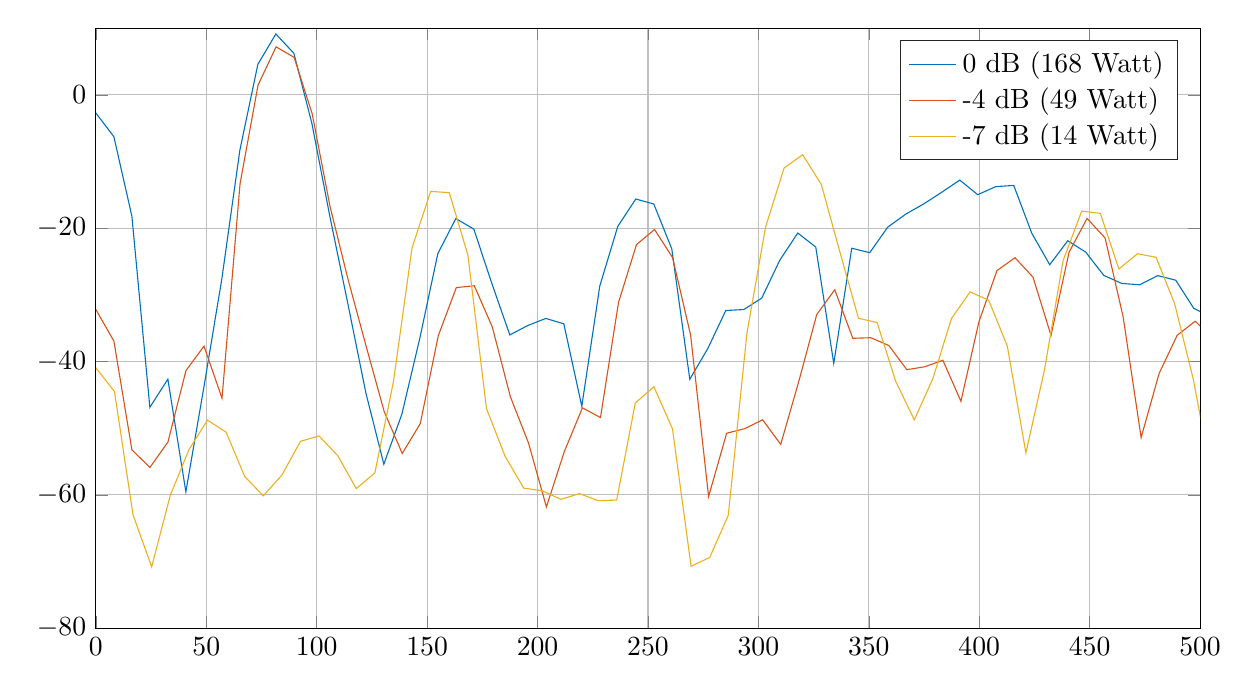
\begin{tikzpicture}

\begin{axis}[%
width=5.521in,
height=3in,
at={(0.758in,0.481in)},
scale only axis,
xmin=0,
xmax=500,
xmajorgrids,
ymin=-80,
ymax=10,
ymajorgrids,
legend style={legend cell align=left,align=left,draw=white!15!black},
axis background/.style={fill=white}
]
\addplot [color=mycolor1,solid]
  table[row sep=crcr]{%
0	-2.72268775884611\\
8.14940577249576	-6.26988319208873\\
16.2988115449915	-18.1821151406506\\
24.4482173174873	-46.863768959253\\
32.597623089983	-42.6455364468348\\
40.7470288624788	-59.5368114060038\\
48.8964346349745	-43.8706429700194\\
57.0458404074703	-27.5795399624388\\
65.195246179966	-8.30946410457154\\
73.3446519524618	4.57461677436454\\
81.4940577249576	9.13428991672223\\
89.6434634974533	6.2503063062714\\
97.7928692699491	-4.24425592410295\\
105.942275042445	-18.2148657363941\\
114.091680814941	-31.3064606471045\\
122.241086587436	-44.6810226835013\\
130.390492359932	-55.3963824675683\\
138.539898132428	-47.9172209172238\\
146.689303904924	-36.5028564595881\\
154.838709677419	-23.8170590268627\\
162.988115449915	-18.5529762112465\\
171.137521222411	-20.1321617146917\\
179.286926994907	-28.2722284420002\\
187.436332767402	-36.0089755301118\\
195.585738539898	-34.5931305686761\\
203.735144312394	-33.5340762775822\\
211.88455008489	-34.3410102716535\\
220.033955857385	-46.7074499002757\\
228.183361629881	-28.6644511072616\\
236.332767402377	-19.7219684577078\\
244.482173174873	-15.620189887388\\
252.631578947368	-16.3662925324231\\
260.780984719864	-23.0989059727317\\
268.93039049236	-42.6549761616301\\
277.079796264856	-38.0556199863087\\
285.229202037351	-32.3461770529013\\
293.378607809847	-32.2006672846573\\
301.528013582343	-30.4795113319134\\
309.677419354839	-24.8040917404552\\
317.826825127334	-20.72407333386\\
325.97623089983	-22.82133087695\\
334.125636672326	-40.2804611122257\\
342.275042444822	-22.9995457941798\\
350.424448217317	-23.6707811970364\\
358.573853989813	-19.8378448608139\\
366.723259762309	-17.8862931571009\\
374.872665534805	-16.3514437097079\\
383.022071307301	-14.607464926372\\
391.171477079796	-12.7803545197056\\
399.320882852292	-14.9694455875423\\
407.470288624788	-13.7610662455677\\
415.619694397284	-13.5810624033614\\
423.769100169779	-20.7382143026417\\
431.918505942275	-25.4780923716951\\
440.067911714771	-21.882767441636\\
448.217317487267	-23.5859028511104\\
456.366723259762	-27.072169806866\\
464.516129032258	-28.2818390526744\\
472.665534804754	-28.4849889563157\\
480.81494057725	-27.1089069764822\\
488.964346349745	-27.7968709337096\\
497.113752122241	-32.0034956949837\\
505.263157894737	-33.3669402365593\\
};
\addlegendentry{0 dB (168 Watt)};

\addplot [color=mycolor2,solid]
  table[row sep=crcr]{%
0	-32.1957485536602\\
8.16048962937776	-36.9378667791654\\
16.3209792587555	-53.2535820990677\\
24.4814688881333	-55.887135861475\\
32.6419585175111	-52.0631872714918\\
40.8024481468888	-41.3588642386764\\
48.9629377762666	-37.6901093730318\\
57.1234274056443	-45.5041279882618\\
65.2839170350221	-13.335087013124\\
73.4444066643999	1.47656576807473\\
81.6048962937776	7.20469310098392\\
89.7653859231554	5.62619917834858\\
97.9258755525332	-2.80723309841304\\
106.086365181911	-16.8215419249471\\
114.246854811289	-27.7541219300966\\
122.407344440666	-37.7371668598206\\
130.567834070044	-47.520638276511\\
138.728323699422	-53.7941043590831\\
146.8888133288	-49.3066037227721\\
155.049302958177	-36.1255117421197\\
163.209792587555	-28.9078832229462\\
171.370282216933	-28.6267637370252\\
179.530771846311	-34.8406626829389\\
187.691261475689	-45.2768594624648\\
195.851751105066	-52.1688721282341\\
204.012240734444	-61.8137102786289\\
212.172730363822	-53.4498730143287\\
220.3332199932	-46.9422189005296\\
228.493709622577	-48.4067331988471\\
236.654199251955	-31.1365453750001\\
244.814688881333	-22.4513381847728\\
252.975178510711	-20.1932676901884\\
261.135668140088	-24.3977816509135\\
269.296157769466	-36.0181599754014\\
277.456647398844	-60.2421620719426\\
285.617137028222	-50.7525219508675\\
293.777626657599	-50.0679547526664\\
301.938116286977	-48.7466838825911\\
310.098605916355	-52.429537262743\\
318.259095545733	-43.022404777189\\
326.419585175111	-32.951108104561\\
334.580074804488	-29.2233203080262\\
342.740564433866	-36.5132810752078\\
350.901054063244	-36.4243948453676\\
359.061543692622	-37.598079883388\\
367.222033321999	-41.223504256542\\
375.382522951377	-40.7767562551518\\
383.543012580755	-39.8079754278704\\
391.703502210133	-45.9660044017571\\
399.86399183951	-34.025063391641\\
408.024481468888	-26.3586540775277\\
416.184971098266	-24.4266615962602\\
424.345460727644	-27.3409100640957\\
432.505950357021	-36.0766670524172\\
440.666439986399	-23.6076962264951\\
448.826929615777	-18.5341492192163\\
456.987419245155	-21.4684460013885\\
465.147908874532	-33.2834506724278\\
473.30839850391	-51.4041406860949\\
481.468888133288	-41.7702381577057\\
489.629377762666	-36.0628345323137\\
497.789867392044	-33.9523443293345\\
505.950357021421	-36.492157579368\\
};
\addlegendentry{-4 dB (49 Watt)};

\addplot [color=mycolor3,solid]
  table[row sep=crcr]{%
0	-40.9386532536309\\
8.42253026846815	-44.4944933967671\\
16.8450605369363	-63.0256778616475\\
25.2675908054045	-70.7944892869375\\
33.6901210738726	-60.0670375347564\\
42.1126513423408	-53.2360039828152\\
50.5351816108089	-48.7846499287097\\
58.9577118792771	-50.5863510384803\\
67.3802421477452	-57.2338859345986\\
75.8027724162134	-60.1412825340367\\
84.2253026846815	-57.0318481289745\\
92.6478329531497	-51.9663475808706\\
101.070363221618	-51.1560740685425\\
109.492893490086	-54.1068331175107\\
117.915423758554	-59.0555621282526\\
126.337954027022	-56.6990432479895\\
134.76048429549	-42.9742061875818\\
143.183014563959	-22.9089021640379\\
151.605544832427	-14.4774590019055\\
160.028075100895	-14.6669647448466\\
168.450605369363	-24.0117810408479\\
176.873135637831	-47.0514815411358\\
185.295665906299	-54.2066808175151\\
193.718196174768	-58.9819603415025\\
202.140726443236	-59.3794637800992\\
210.563256711704	-60.6745985915569\\
218.985786980172	-59.8046744958017\\
227.40831724864	-60.8734896250765\\
235.830847517108	-60.7774814693277\\
244.253377785576	-46.2214075395246\\
252.675908054045	-43.7808373144067\\
261.098438322513	-50.0960412265735\\
269.520968590981	-70.7077749367099\\
277.943498859449	-69.3917839929786\\
286.366029127917	-63.0592863364453\\
294.788559396385	-35.7869367132467\\
303.211089664853	-19.8663193549835\\
311.633619933322	-10.964236294141\\
320.05615020179	-8.98332835764642\\
328.478680470258	-13.4375057819054\\
336.901210738726	-23.5620775763145\\
345.323741007194	-33.5135511530661\\
353.746271275662	-34.1445168550196\\
362.168801544131	-42.9570284983663\\
370.591331812599	-48.7543483503136\\
379.013862081067	-42.5458679897274\\
387.436392349535	-33.5384633473077\\
395.858922618003	-29.5475304778267\\
404.281452886471	-30.8057291729961\\
412.703983154939	-37.6728501979446\\
421.126513423408	-53.7025004354437\\
429.549043691876	-41.2380146003191\\
437.971573960344	-24.8559922101925\\
446.394104228812	-17.4380502514164\\
454.81663449728	-17.7657729900535\\
463.239164765748	-26.1108922525535\\
471.661695034217	-23.8265363694278\\
480.084225302685	-24.3638075864788\\
488.506755571153	-31.3509006667339\\
496.929285839621	-42.6724931603654\\
505.351816108089	-57.4173187030205\\
};
\addlegendentry{-7 dB (14 Watt)};
\end{axis}


\end{tikzpicture}%
	\caption{Caption }
	\label{fig:FFTAcceptTest}
\end{figure}

\section{Error sources}

Few errors could have occurred during trials, since then only variable adjusted during between measurements were the gain of the amplifier. There were however problems with moving the setup from the control room were it was calibrated and then moved into the anechoic room. The calibration was done using an visual equalizer where the output was shown with a bar chart Hence the data should bee seen with a tolerance of +/- 0.5 dB.


\section{Conclusion}

It can be concluded that the signal no longer creates a hit against the back plate. This was present before at the same amplitudes. The signal has now been attenuate enough to suppress these spikes. however the characteristics of the signal remains the same, even at higher amplitudes. It should however be noted that the trials were conducted in a scaled scenario where the gain of the amplifier was dampen by 3 dB, which would make the system activate at a lower threshold than 150 watts.  
